%%=============================================
% !Mode:: "TeX:UTF-8"
% !TEX program  = XeLaTeX
%%=============================================
% 模板名称:hitszthesis
% 模板版本:V3.2.3
% 模板作者:杨敬轩(Jingxuan Yang)
% 联系作者:yangjx20@mails.tsinghua.edu.cn & yanglatex2e@gmail.com
% 模板交流:QQ群:1039392552,加群请备注LaTeX、hitszthesis相关说明
% 模板适用:哈尔滨工业大学(深圳)本、硕、博学位论文
% 模板编译:手动编译方法参看 README.md 或 hitszthesis.pdf
%          GNU make 工具:make thesis
%          Windows 批处理脚本:双击 compile.bat 自动编译论文
%          更多编译细节详见说明文档:hitszthesis.pdf
% 更新时间:2022/05/05
% 模板帮助:请**务必务必务必**阅读 hitszthesis.pdf 说明文档,文档查看方法:
%          cmd 命令行:texdoc hitszthesis
%          推荐前往模板的 GitHub 仓库获取最新文件,地址:
%          https://github.com/YangLaTeX/hitszthesis
%%=============================================

% 设置文档类别为 <hitszthesis>
% \documentclass[type=doctor]{hitszthesis}
% \documentclass[type=master]{hitszthesis}
\documentclass[type=bachelor,infoleft=true]{hitszthesis}

% 模板提供以下选项,各个选项之间不要有空格
% 1. type=bachelor|master|doctor
%   含义:本科、硕士、博士学位论文,不设默认值,**必填**
% 2. covertitletworow=true|false
%   含义:本科封面第一页标题单行或多行显示,默认为单行显示(false)
% 3. infoleft=true|false
%   含义:本科封面第二页下划线内容居中或居左显示,默认为居中显示(false)
% 4. mathfont=newtxmath|mtprotwolite|mtprotwo
%   含义:正文数学字体选项:newtxmath(默认),mtprotwolite(lite版,免费),
%         mtprotwo(完全版,需购买授权),
%         mtpro2字体官网:https://www.pctex.com/mtpro2.html
% 5. boldcaption=true|false
%   含义:图表题注是否加粗,默认为不加粗(false)
% 6. tocfour=true|false
%   含义:是否添加第四级目录,只对本科文科个别要求四级目录有效,默认不添加(false)
% 7. fulltime=true|false
%   含义:是否全日制,非全日制如同等学力等,要在coverinformation中设置类型,
%        默认是全日制(true)
% 8. subtitle=true|false
%   含义:论文题目是否含有副标题,默认没有副标题(false)
% 9. openright=true|false
%   含义:博士论文是否要求章节首页必须在奇数页,默认否(false)
% 10. library=true|false
%   含义:是否为提交到图书馆的电子版,默认否(false)
% 11. alphappendix=true|false
%   含义:本科毕业设计附录章节编号是否为大写字母,默认是(true)

% 自定义设置与额外加载的宏包请写在 \file{hitszthesis.sty} 里
\usepackage{hitszthesis}

% 图片存放路径,在这些文件夹里的图片可以直接使用图片文件名调用
\graphicspath{{figures/}{pictures/}}

%%=============================================
% 开始写论文
% !!注意本文仅作为排版格式示例,并不作为毕业论文规范
\begin{document}

% 若题目过长,则需使用以下命令调整本科封面第二页下划线长度
%\infowidth = 9cm

% 开始写前言部分
\frontmatter

% 封面信息填写
% !TEX root = ../main.tex

\hitszsetup{
  %******************************
  % 注意:
  %   1. 配置里面不要出现空行
  %   2. 不需要的配置信息可以删除
  %******************************
  %
  %=====
  % 秘级
  %=====
  statesecrets={公开},
  natclassifiedindex={TM301.2},
  intclassifiedindex={62-5},
  %
  %=========
  % 中文信息
  %=========
  ctitleone={过驱动飞行器的轨迹},%本科生封面使用
  ctitletwo={规划},%本科生封面使用
  ctitlecover={过驱动飞行器的轨迹规划},%放在封面中使用,自由断行
  ctitle={过驱动飞行器的轨迹规划},%放在原创性声明中使用
  csubtitle={一条副标题}, %一般情况没有,可以注释掉
  cxueke={工学},
  cpostgraduatetype={学术},
  csubject={自动化},
  % csubject={机械工程},
  caffil={机电工程与自动化学院},
  % caffil={哈尔滨工业大学(深圳)},
  cauthor={刘培焱},
  csupervisor={陈浩耀 教授},
  cassosupervisor={某某某 教授}, % 副指导老师
  % ccosupervisor={某某某 教授}, % 联合指导老师
  % 日期自动使用当前时间,若需指定按如下方式修改:
  cdate={2022年6月},
  % 指定第二页封面的日期,即答辩日期
  cdatesecond={2022年06月10日},
  cstudentid={180310211},
  cstudenttype={同等学力人员}, %非全日制教育申请学位者
  %(同等学力人员)、(工程硕士)、(工商管理硕士)、
  %(高级管理人员工商管理硕士)、(公共管理硕士)、(中职教师)、(高校教师)等
  %
  %
  %=========
  % 英文信息
  %=========
  etitle={Research on robot intelligent grasping based on Neural Network},
  esubtitle={This is the sub title},
  exueke={Engineering},
  esubject={Mechanical Engineering},
  eaffil={Harbin Institute of Technology, Shenzhen},
  eauthor={Jingxuan Yang},
  esupervisor={Prof. XXX},
  % eassosupervisor={XXX},
  % 日期自动生成,若需指定按如下方式修改:
  edate={June, 2020},
  estudenttype={Master of Engineering},
  %
  % 关键词用“英文逗号”分割
  ckeywords={过驱动飞行器, 轨迹规划, 避障},
  ekeywords={over-actuated aircraft, trajectory planning, obstacle avoidance},
}

% 中文摘要
\begin{cabstract}

  全向多旋翼无人飞行器是近年来正在发展的一个研究领域。作为一种全向系统,
        全向多旋翼飞行器具有传统欠驱动多旋翼飞行器相比更加灵活的机动性,其在狭小
        空间中的避障飞行也具有更大的优势。本文中我们为全向六旋翼飞行器设计了一个
        基于优化的六自由度轨迹规划器,本规划器在欠驱动四旋翼飞行机的SE(3)运动规
        划方案的基础上根据全向六旋翼飞行器的特点进行改进,用一系列凸多面体表示
        环境中的安全区域,得到一条包含位置坐标和表示机体姿态的六自由度
        无碰撞轨迹。并进行了仿真实验验证了可行性。

\end{cabstract}

% 英文摘要
\begin{eabstract}
  Omnidirectional multirotor uav is a developing research 
  field in recent years. As an omnidirectional system, 
  omnidirectional multi-rotor aircraft has more flexible 
  maneuverability than traditional underactuated multi-rotor 
  aircraft, and it also has greater advantages in obstacle 
  avoidance flight in narrow space. In this paper, 
  we design a six-degree of freedom trajectory planner 
  based on optimization for omnidirectional six-rotor aircraft.
   Based on the SE(3) motion planning scheme of underactuated 
   four-rotor aircraft, the planner is improved according to the
    characteristics of omnidirectional six-rotor aircraft. 
    A series of convex polyhedra are used to represent the
     safety zone in the environment. A 6 dof collision-free 
     trajectory containing position coordinates and body attitude 
     is obtained. The feasibility is verified by simulation 
     experiments.

\end{eabstract}


% 生成封面、中英文摘要
\makecover

% 物理量名称表,若采用标准符号则不需要此表
% % !TEX root = ../main.tex

% 物理量符号表,如果采用标准符号则不需要此表
\begin{denotation}
  % 此处最好是h
  \begin{table}[h]
  \caption{国际单位制中具有专门名称的导出单位}
  \vspace{0.5em}\centering\wuhao
  \begin{tabular}{ccccc}
    \toprule[1.5pt]
    量的名称&单位名称&单位符号&其它表示实例\\
    \midrule[0.2pt]
    频率&赫[兹]&Hz&s-1\\
    \bottomrule[1.5pt]
    \end{tabular}
  \end{table}
\end{denotation}


% 中文目录
\tableofcontents

% 英文目录,本硕不要求
% \tableofengcontents

% 开始写正文
\mainmatter

% 第1章
% !TEX root = ../main.tex

% 中英标题:\chapter{中文标题}[英文标题]
\chapter{绪\ 论}[Introduction]

\section{课题背景及研究的目的和意义}[Background, objective and significance of the subject]

% 正文内容,注意LaTeX分段有两种方法,直接空一行或者使用<\par>
% 默认首行缩进,不需要在代码编辑区手动敲空格
\subsection{课题背景}
近些年来,随着控制科学、感知导航以及人工智能等技术的不断进步,关于多旋翼无人机(multirotor UAV)的设计及应用的领域展现出了空前的繁荣,并取得了长足的发展。
多旋翼无人机凭借其简洁的机械结构以及优秀的飞行稳定性,从一众智能机器人中脱颖而出,从实验室里走进了千家万户。
在许多地方,如日常生活中的航拍,或是农林、检修和军事行动等特种作业场合中,都有多旋翼无人机的用武之地(\figref{fig:applications})。

\begin{figure}[!ht]
    \setlength{\subfigcapskip}{-1bp}
    \centering
    \begin{minipage}{\textwidth}

    \centering
    \subfigure{\label{fig:aerial_photo}}\addtocounter{subfigure}{-2}
    \subfigure{\subfigure[用于航拍测绘]{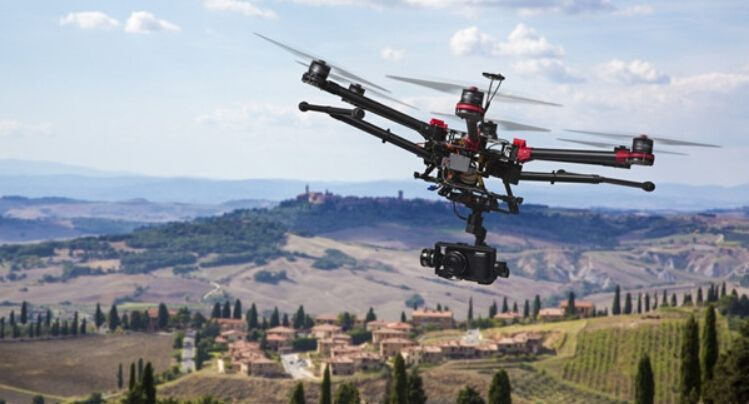
\includegraphics[width=0.45\textwidth, height=0.25\textwidth]{aerial_photo.jpeg}}}
    \hspace{0.2em}
    \subfigure{\label{fig:farming}}\addtocounter{subfigure}{-2}
    \subfigure{\subfigure[用于农林植保]{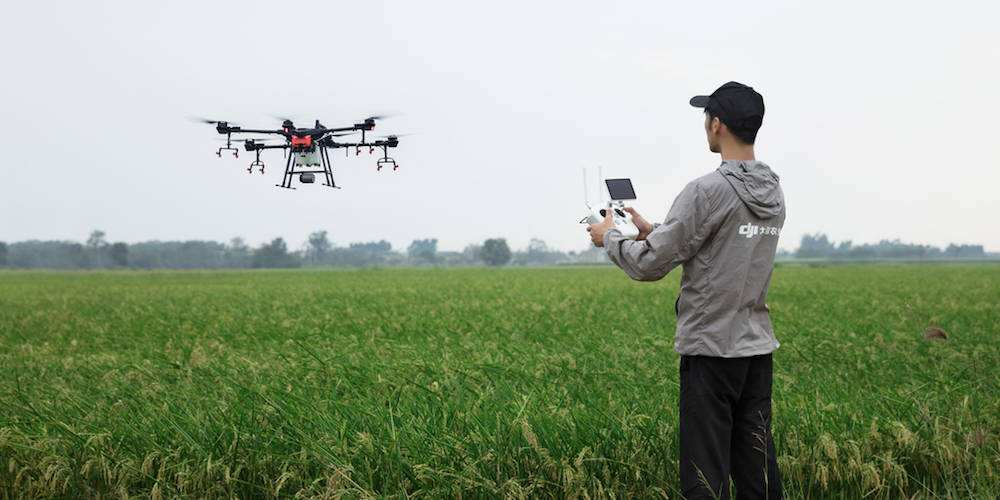
\includegraphics[width=0.45\textwidth, height=0.25\textwidth]{farming.jpeg}}}

    \subfigure{\label{fig:inspection}}\addtocounter{subfigure}{-2}
    \subfigure{\subfigure[用于电力巡检]{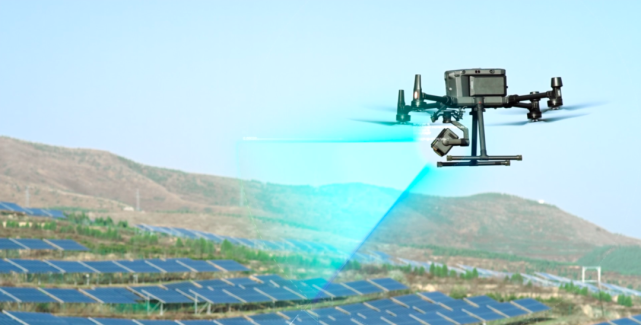
\includegraphics[width=0.45\textwidth, height=0.25\textwidth]{inspection.jpeg}}}
    \hspace{0.2em}
    \subfigure{\label{fig:logistics}}\addtocounter{subfigure}{-2}
    \subfigure{\subfigure[用于后勤补给]{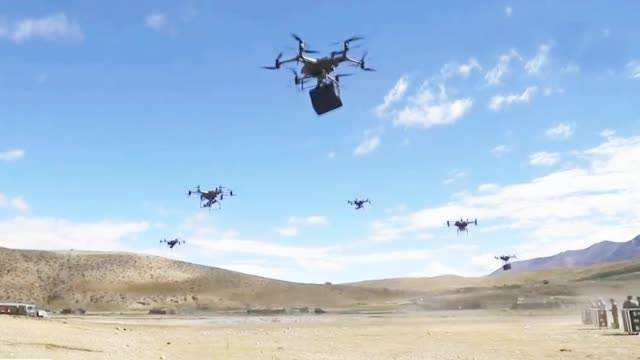
\includegraphics[width=0.45\textwidth, height=0.25\textwidth]{logistics.jpeg}}}
    
    \end{minipage}
    \caption{多旋翼无人机的多种应用场景}
    \label{fig:applications}
\end{figure}

然而,从机械结构中可以发现,目前所应用的大多数多旋翼无人机的各个旋翼的转轴均互相平行且垂直于机身平面,所以旋翼只能为飞行器提供垂直机身平面的推力。
这就使得飞行器成为一个欠驱动系统(under-actuated system)\cite{underactuated},其位置控制和姿态控制是耦合的。
具体表现为,如果飞行器需要水平飞行,则必须倾斜机身才能获得水平方向的分力,以提供水平方向的加速度和克服空气阻力;
类似地,飞行器只有在水平姿态下才可以保持悬停。
这种特性很大程度上限制了欠驱动多旋翼飞行器的应用场景:
在空中作业时,悬停姿态的限制会使飞行器无法克服机载机械臂或机载云台的机械死角;
在拥挤的环境中,姿态与推力的耦合也会严重削弱飞行器的避障性能,使环境中的可行区域大幅缩减。

为了改善上述问题,充分发掘多旋翼飞行器的潜力,近年来发展出了多种能将飞机的位置与姿态控制解耦的多旋翼飞行器。
这些工作通过改变旋翼几何构型、增加旋翼倾转自由度等方式让旋翼能提供相对机身任意方向的推力和转矩,这赋予了多旋翼飞行器跟踪6自由度全状态轨迹的能力,使飞行器成为全驱动系统(fully actuated system)。
这种飞行器能够分别独立地进行平移和旋转运动,故又称为全向飞行器(omnidirectional aerial vehicle),这种受控的、自由的刚体运动是传统欠驱动多旋翼飞行器所无法做到的。
所谓过驱动飞行器,就是具有冗余控制输入(驱动器)的全驱动飞行器,在少数驱动器故障的情况下依然能够进行控制,增强了飞行器的容错能力。


\subsection{研究的目的和意义}
由于上述过驱动多旋翼飞行器的位置和姿态可以独立控制,故可以为其独立规划位置和姿态共6个自由度的轨迹,其飞行的灵活性相比于只能跟踪4自由度轨迹的传统欠驱动多旋翼飞行器将大幅提高。
设想当面对一个狭长笔直、宽度小于自身旋翼间最小距离的通道时,加速度与姿态耦合的欠驱动飞行器显然无法通过;
而过驱动飞行器则可以通过控制姿态使机身倾斜以适应通道内的狭小空间,同时控制位置从而实现平稳无碰撞的穿越。
这样的优势使得过驱动飞行器在未知环境探索、巷战侦查与打击、灾区废墟搜救等场合势必会发挥出很大的应用价值。
要更好地挖掘过驱动多旋翼飞行器的潜力、提高其自主飞行性能,为其设计一套在复杂狭小空间内进行避障轨迹规划的算法是具有重要意义的。

本文以实现过驱动多旋翼飞行器在复杂环境中的避障飞行为目标,对基于过驱动多旋翼飞行器的$SE(3)$运动规划算法展开研究,设计了一个考虑飞行器整体形状和动力学约束的全局轨迹规划器,
并设计仿真和实物实验验证了所设计规划器的可行性,为相关领域探索了一条可行的道路,且有望后续通过并行计算及对算法进行优化等手段,配合机载感知系统实现实时规划。


\section{国内外研究现状}[Developmental of gas-lubricated bearing and correlated theories]
轨迹规划模块处于无人机软件框架的中间位置,其接收感知模块传来的地图等上游信息,输出一条安全、平滑的可行轨迹输送给控制模块。
规划模块起到了承上启下的作用,可以说是影响无人机自主飞行性能的最重要的一环;
另外,在多旋翼飞行器全驱动化方面,目前也有不少种方案可以参考。
本节将从欠驱动多旋翼飞行器的避障轨迹规划、过驱动多旋翼飞行器和过驱动多旋翼飞行器的轨迹规划三方面讲述国内外研究现状。

\subsection{欠驱动多旋翼飞行器的避障轨迹规划}
多旋翼飞行器的避障轨迹规划这一领域近年来取得了丰富的成果。
大多数多旋翼飞行器属于微分平坦系统(differential flat system)\cite{2003Flatness},这种系统的运动规划问题可以在保证一定的平滑性的前提下转化为较低维度的优化问题,
其平坦输出的轨迹可以表示为分段多项式,这样就能方便地获得轨迹关于时间的各阶导数,进而利用微分平坦关系求得飞行器的各状态变量和控制输入。

2011年,Mellinger等人提出了为四旋翼飞行器生成固定间隔多项式轨迹的方法\cite{2011minimumsnap},通过求解一个由加速度的二阶导数(即snap)的平方积分代价以及线性安全约束构造的二次规划(Quadratic Programming,QP)问题,最终生成一条平滑且安全的轨迹。
2015年,Bry等人推导出了导数平方积分形式无约束二次规划问题的闭式解\cite{bry2015aggressive},并且启发式地在前端RRT*搜索出的可行路径上添加路点直到无碰撞为止,以此来保证轨迹的安全性。
\begin{figure}[!ht]
    \setlength{\subfigcapskip}{-1bp}
    \centering
    \begin{minipage}{\textwidth}

    \centering
    \subfigure{\label{fig:ttr_corridor}}\addtocounter{subfigure}{-2}
    \subfigure{\subfigure[生成的安全飞行走廊]{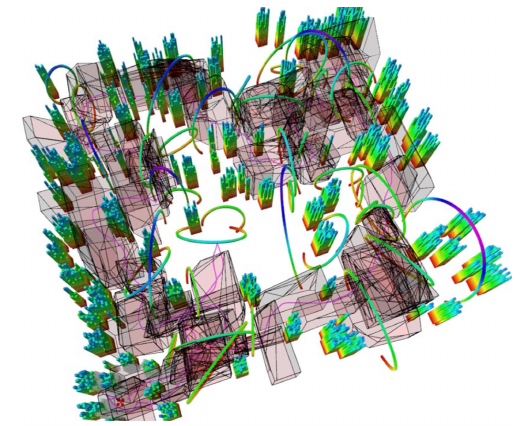
\includegraphics[width=0.4\textwidth, height=0.4\textwidth]{gao2020teach_a.png}}}
    \hspace{0.2em}
    \subfigure{\label{fig:ttr_trajectory}}\addtocounter{subfigure}{-2}
    \subfigure{\subfigure[经过优化的轨迹]{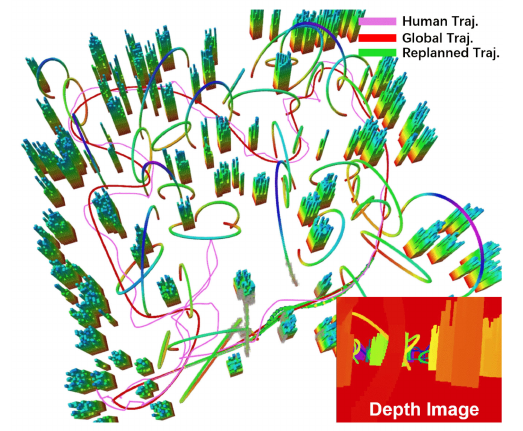
\includegraphics[width=0.4\textwidth, height=0.4\textwidth]{gao2020teach_b.png}}}
    
    \end{minipage}
    \caption{Teach-Repeat-Replan示意图\cite{gao2020teach}}
    \label{fig:TTR}
\end{figure}
2020年,Gao等人将环境中的安全区域表示为凸多面体\cite{gao2020teach},一系列凸多面体连接起来构成安全飞行走廊(safe flight corridor,SFC)(\figref{fig:TTR}),轨迹的安全性由B\'{e}zier曲线的凸包性质来保证。
2021年,Zhou等人提出了EGO-Planner,与多数基于梯度的轨迹规划方法不同,EGO-Planner直接从障碍物上获得梯度信息,从而免去了对ESDF地图的依赖,大大降低了内存消耗和计算量。

\begin{figure}[ht]
    \centering
    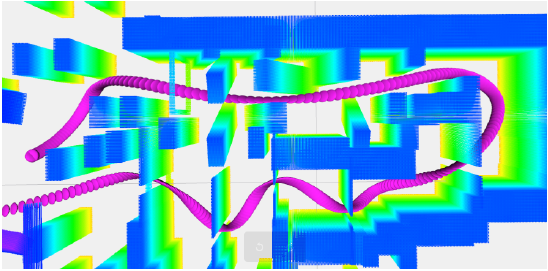
\includegraphics[width = 0.65\textwidth]{se3_traj.png}
    \caption{在$SE(3)$空间中规划出的轨迹\cite{2021Fast}}
    \label{fig:se3_traj}
\end{figure}

以上工作都能高效地进行轨迹规划,然而它们都是在构型空间(configuration space)中进行规划,并未考虑无人机的几何形状和姿态,具有很大的保守性。
在某些比较极端的环境中,存在需要无人机倾斜机身才能飞过的狭窄缝隙,此时传统的$\mathbb{R}^3$规划器是难以发挥作用的。
要得到如\figref{fig:se3_traj}所示通过改变姿态以实现在较为拥挤的环境中无碰撞的安全轨迹,就需要在$SE(3)$空间中进行规划。
2018年,Liu等人提出了一种基于搜索的$SE(3)$规划算法\cite{liu2018search},其通过在一定的时间间隔内施加常量控制输入来生成运动基元(motion primitive),配合可行性检测器筛选出与点云无交集的运动基元,最终搜索出一条无碰撞轨迹。
不过,该算法存在着组合爆炸(combinatorial explosion)问题:要想获得更高的求解质量,就得提高分辨率,而随着分辨率的增高,计算量会快速增加,带来不可接受的计算时间和内存消耗,故这种算法实用性欠佳。

2022年,Wang等人提出了一个几何约束下的多旋翼飞行器轨迹优化框架\cite{wang2022geometrically}。该框架首先基于多阶段最优控制问题的最优充要条件,构建了名为MINCO的一类分段多项式轨迹,这类轨迹以其必须经过的中间点和每段的时间分配作为参数,轨迹的系数矩阵可以根据最优条件以线性的时间和空间复杂度计算出来,这相较Bry等人提出的闭式解\cite{bry2015aggressive}有了很大改进;
使用MINCO轨迹类,就可以直接对中间点和时间分配进行优化,同时还能保证轨迹的平滑性。
该框架还通过一系列技巧消去了对时间分配的约束以及对中间点的空间约束,并将其余自定义约束软化为目标函数中的惩罚项,最终将整个带约束的轨迹优化问题转化为无约束优化问题,得以高效求解。
该框架的提出为$SE(3)$规划问题提供了新思路,紧接着Yang等人构造了考虑四旋翼飞行器的形状与姿态,并使飞行器整体包含在表示安全区域的凸多面体内的约束形式\cite{yang2021whole},该约束作为框架中的自定义约束来处理;Han等人进一步开发了用于无人机竞速的$SE(3)$规划器\cite{2021Fast},并将其开源\footnote{https://github.com/ZJU-FAST-Lab/Fast-Racing}。


\subsection{过驱动多旋翼飞行器}[Developmental of gas-lubricated bearing]
实现多旋翼飞行器全驱动化的要点在于使驱动器同时且独立地产生相对机体任意方向推力和力矩,而要做到这一点需要改变旋翼的构型(configuration of rotors)。
过驱动全向多旋翼飞行器领域近年来正处于持续发展中,这些全向飞行器按照旋翼构型大致可分为两类:固定旋翼型(fixed-rotor)\cite{brescianini2016design, park2018odar,allenspach2020design}和倾转旋翼型(tiltrotor)\cite{ryll2014novel, kamel2018voliro,2021Geometrically}。
\figref{fig:omav}分别展示了两种构型中具有代表性的一项工作。

\begin{figure}[!ht]
    \setlength{\subfigcapskip}{-1bp}
    \centering
    \begin{minipage}{\textwidth}

    \centering
    \subfigure{\label{fig:omav_1}}\addtocounter{subfigure}{-2}
    \subfigure{\subfigure[固定旋翼型\cite{brescianini2016design}]{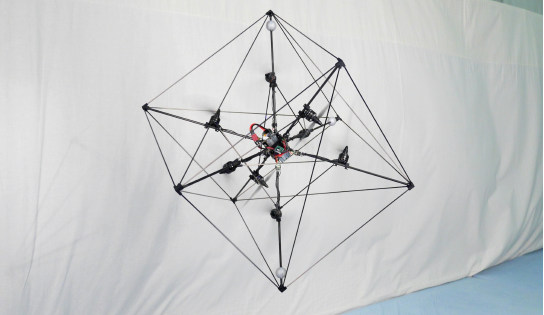
\includegraphics[width=0.4\textwidth]{octo_omav.png}}}
    \hspace{0.2em}
    \subfigure{\label{fig:omav_2}}\addtocounter{subfigure}{-2}
    \subfigure{\subfigure[可倾转旋翼型\cite{kamel2018voliro}]{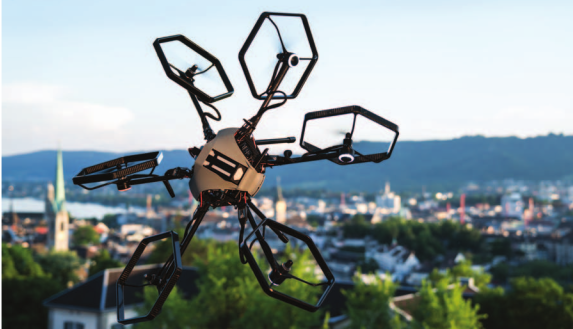
\includegraphics[width=0.4\textwidth]{voliro_2.png}}}
    
    \end{minipage}
    \caption{两种不同种类旋翼构型的全向多旋翼飞行器示例\label{fig:omav}}
\end{figure}

固定旋翼的过(全)多旋翼飞行器的机械结构相对简单,飞行器通过改变不同朝向旋翼的转速来控制推力和转矩的大小和方向。
如\figref{fig:omav_1}所示为Brescianini等人于2016年发表的一种实现灵活全向飞行的固定旋翼型八旋翼飞行器系统\cite{brescianini2016design},
该系统采用8个可逆电机-旋翼组合执行器(reversible motor-propeller actuator),故每个执行器都可以产生正推力和负推力,
8个执行器的构型是基于静态力和扭矩分析,采用求解优化问题的方式来设计的,以期最大化飞行器的灵活性并最大限度保证飞行器动力学特性的旋转不变性。
不过,固定旋翼型的过驱动飞行器的一个主要缺点在于:这些旋翼通常不会同时直接朝向竖直方向,使得这类飞行器的悬停效率不会很高;
并且如果设定旋翼朝向使之更倾向于高效的悬停和更高的有效载荷,就会几乎不可避免地降低产生横向作用力的能力\cite{allenspach2020design}。

可倾转旋翼型全向多旋翼飞行器的实现方式多数是为旋翼增加额外的自由度,使其转轴指向可以改变。
比较常用的方式是为安装旋翼的机臂添加一个绕其轴的旋转自由度:
如\figref{fig:tiltrotor_quadrotor}展示了Markus等人于2015年研制出的一种可倾转旋翼的过驱动四旋翼飞行器的结构\cite{ryll2014novel},该飞行器可以在有限的横滚角和俯仰角下实现悬停;
\figref{fig:omav_2}展示的是Kamel等人于2018年开发的一种可倾转旋翼的全向六旋翼飞行器Voliro\cite{kamel2018voliro},该飞行器可以实现任意姿态下的悬停和飞行。
这类飞行器通过改变每个旋翼的朝向,实现了更高效的悬停。
本课题所使用的仿真及实物实验平台是参考Voliro的结构搭建的。

\begin{figure}[ht]
    \centering
    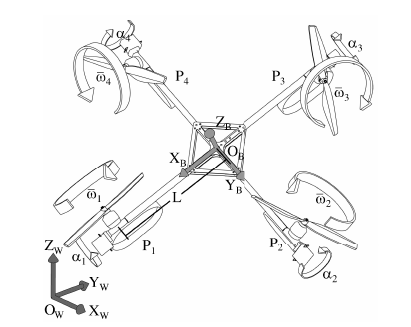
\includegraphics[width = 0.65\textwidth]{omni_quadrotor.png}
    \caption{Markus Ryll等人的可倾转旋翼的全向四旋翼飞行器结构示意图}
    \label{fig:tiltrotor_quadrotor}
\end{figure}

\subsection{过驱动飞行器的轨迹规划}
现有的关于过(全)驱动飞行器的研究主要集中于机械结构设计和飞行控制算法方面,而为过驱动飞行器进行轨迹规划的相关成果并不太多。
2018年,Brescianini等人基于运动基元为过驱动飞行器生成了从给定起点到给定终点且满足一定动力学约束的6自由度轨迹\cite{brescianini2018computationally}。
同年,Morbidi等人提出了用于双轴倾转旋翼六旋翼飞行器的节能轨迹生成方法\cite{morbidi2018energy},通过求解一个显式考虑电机电气模型的优化控制问题得到一条指定边界点的节能轨迹,并做了数值验证。
2021年,Pantic等人提出了基于流形网格的运动规划方法\cite{pantic2021mesh},该方法将物体表面(surface)建模为三角网格(triangular mesh)并提出原始表面的一个低维参数化表示方法,进一步将原始表面及其低维表示近似为流形(manifold),运用黎曼运动策略(Riemannian Motion Policies,RMPs)构建了一个高效且通用的运动规划框架;
该方法目的在于生成一条使飞行器飞向指定表面并沿其飞行,应用于全向飞行器与曲面交互的场景。

\section{本文的主要研究内容}[Main research contents of this subject]
从国内外研究现状中可以看出,目前已有许多成熟的方案能赋予多旋翼无人机跟踪6自由度轨迹、实现全向飞行的能力。
在避障轨迹规划方面,以欠驱动多旋翼飞行器为平台的解决方案同样多样且成熟,其中在复杂空间内进行$SE(3)$避障规划也已经有了效果拔群的成果;
然而,在能够进行全向飞行的过驱动多旋翼飞行器平台上进行轨迹规划的成果并不多,其中多数\cite{brescianini2018computationally, morbidi2018energy}并未考虑障碍物存在情况下的安全约束,Pantic等人的方法\cite{pantic2021mesh}也并不太适用于避障。
事实上,面向复杂环境中过驱动飞行器的$SE(3)$轨迹规划的解决方案几乎还没有已发表的成果。
传统基于欠驱动多旋翼飞行器的轨迹规划方法固然可以应用到过驱动飞行器上,但由于这些方法并不能生成6自由度轨迹,所以它们并不能充分发挥过驱动飞行器的避障潜能。

本文重点研究过驱动多旋翼飞行器在复杂环境中的$SE(3)$轨迹规划。
通过深入研究、对比各种已有的轨迹规划方案,结合过驱动飞行器的不同性质,完成规划算法设计、代码实现、仿真验证及实物验证。
本文主要研究内容如下:
\begin{enumerate}
    \renewcommand{\labelenumi}{(\theenumi)}
    \item 参考过驱动飞行器系统Voliro\cite{kamel2018voliro},搭建了全向六旋翼飞行器OmniHex的仿真和实物模型,并对其动力学模型进行研究和分析。
    \item 针对前端路径搜索和安全飞行走廊生成的问题,研究已有方案和开源代码,设计$SE(3)$空间中的RRT算法用于前端路径搜索,设计凸多面体安全飞行走廊生成算法用于空间约束的生成。
    \item 为实现复杂环境中的6自由度$SE(3)$轨迹规划,对姿态规划方式及后端轨迹优化问题展开研究,设计了基于欧拉角和基于四元数的两种姿态规划方式,并分别设计对应的安全约束和动力学约束形式,推导对应的罚函数及其梯度。
    \item 将所设计的算法实现为C++接口,并对其进行整合,实现为基于ROS\cite{quigley2009ros}的全局规划器,并基于Gazebo\cite{gazebo}和PX4\cite{meier2015px4}进行仿真实验、基于实物平台进行实物实验,以验证其可行性。
\end{enumerate}



% 第2章
% !TEX root = ../main.tex

% 中英标题:\chapter{中文标题}[英文标题]
\chapter{排版图片}[Typesetting pictures]

\section{引言}[Introduction]
图应有自明性。插图应与文字紧密配合,文图相符,内容正确。选图要力求精练,插图、照
片应完整清晰。机械工程图:采用第一角投影法,严格按照GB4457~GB131-83《机械制图》
标准规定。数据流程图、程序流程图、系统流程图等按GB1526-89标准规定。电气图:图形
符号、文字符号等应符合附录3所列有关标准的规定。流程图:必须采用结构化程序并正确
运用流程框图。对无规定符号的图形应采用该行业的常用画法。坐标图的坐标线均用细实线
,粗细不得超过图中曲线;有数字标注的坐标图,必须注明坐标单位。照片图要求主题和主
要显示部分的轮廓鲜明,便于制版。如用放大或缩小的复制品,必须清晰,反差适中。照片
上应有表示目的物尺寸的标度。引用文献中的图时,除在正文文字中标注参考文献序号以外
,还必须在中、英文表题的右上角标注参考文献序号。

\section{博士毕业论文双语题注}[Doctoral picture example]

博士毕业论文双语题注如\figref{golfer1}所示。

\begin{figure}[htpb]
\centering
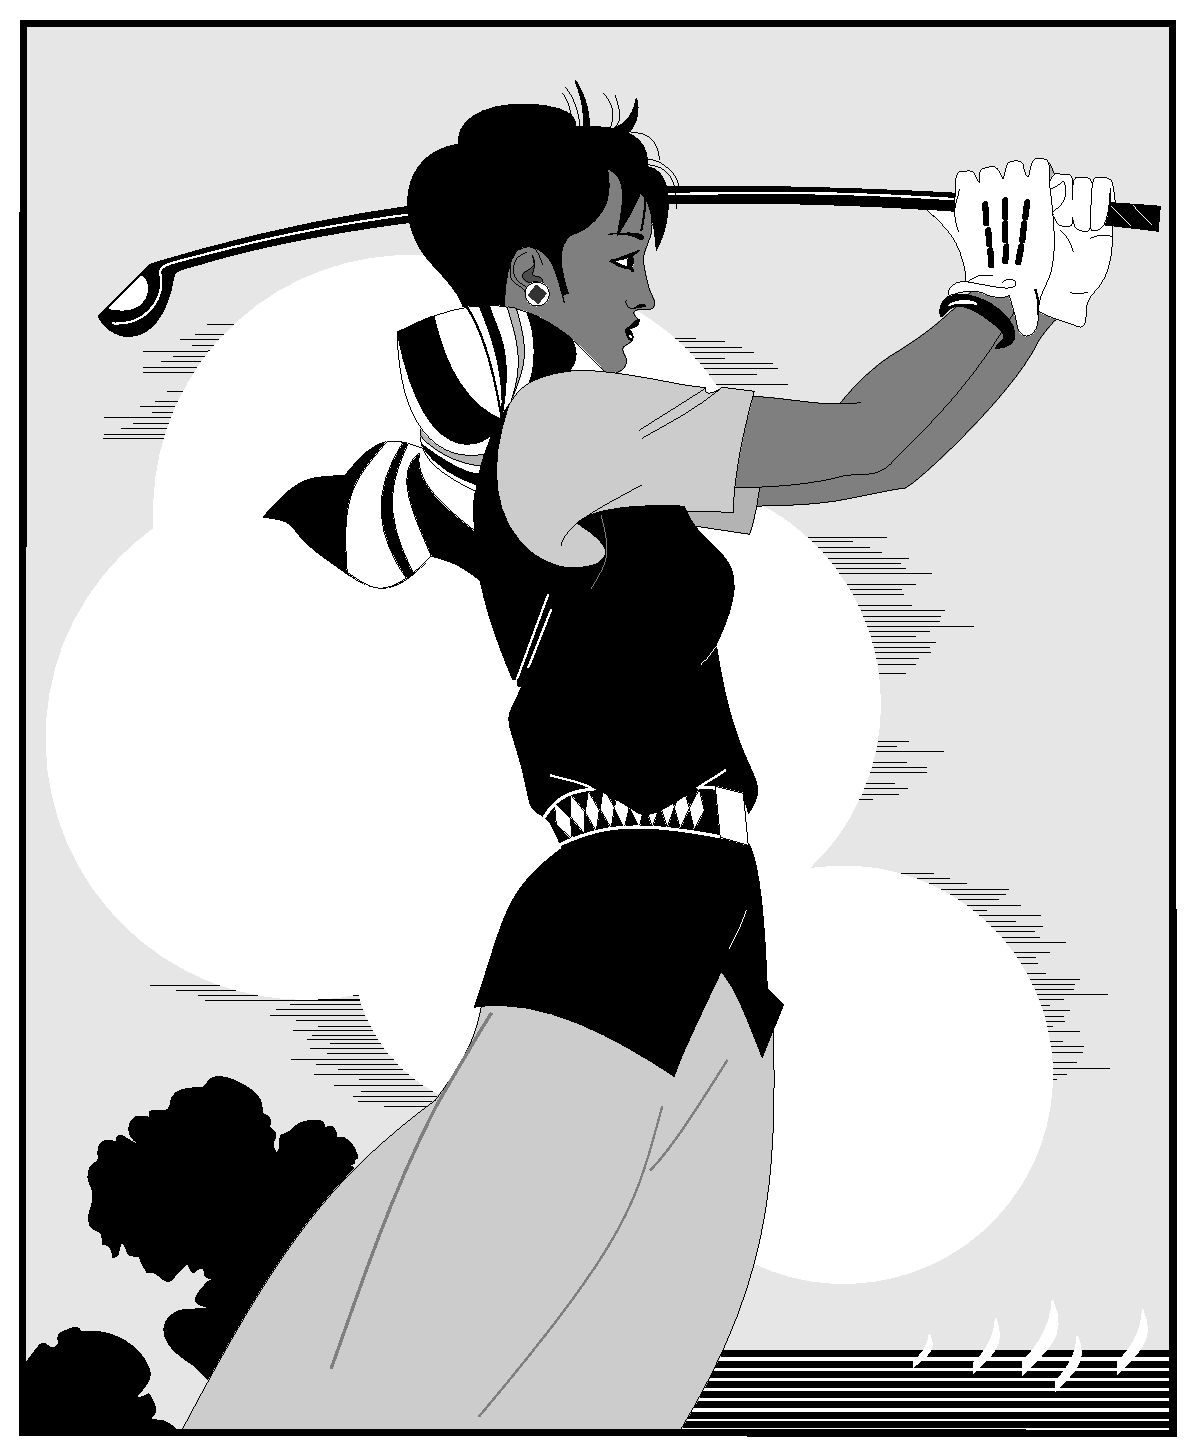
\includegraphics[width = 0.4\textwidth]{golfer}
\bicaption[golfer1]{}{打高尔夫球球的人(博士论文双语题注)}{Fig.$\!$}{The person playing golf (Doctoral thesis)}
\end{figure}

每个图均应有图题(由图序和图名组成),图题不宜有标点符号,图名在图序之后空1个半
角字符排写。图序按章编排,如第1章第一个插图的图号为“图1-1”。图题置于图下,硕士论
文只用中文,博士论文用中、英两种文字,居中书写,中文在上,要求中文用宋体5号字,
英文用Times New Roman 5号字。有图注或其它说明时应置于图题之上。引用图应注明出处
,在图题右上角加引用文献号。图中若有分图时,分图题置于分图之下或图题之下,可以只
用中文书写,分图号用a)、b)等表示。图中各部分说明应采用中文(引用的外文图除外)或
数字符号,各项文字说明置于图题之上(有分图时,置于分图题之上)。图中文字用宋体、
Times New Roman字体,字号尽量采用5号字(当字数较多时可用小5号字,以清晰表达为原
则,但在一个插图内字号要统一)。同一图内使用文字应统一。图表中物理量、符号用斜体
。
\subsection{本硕论文题注}[Other picture example]

本硕论文题注如\figref{fig:bm}所示。

\begin{figure}[ht]
\centering
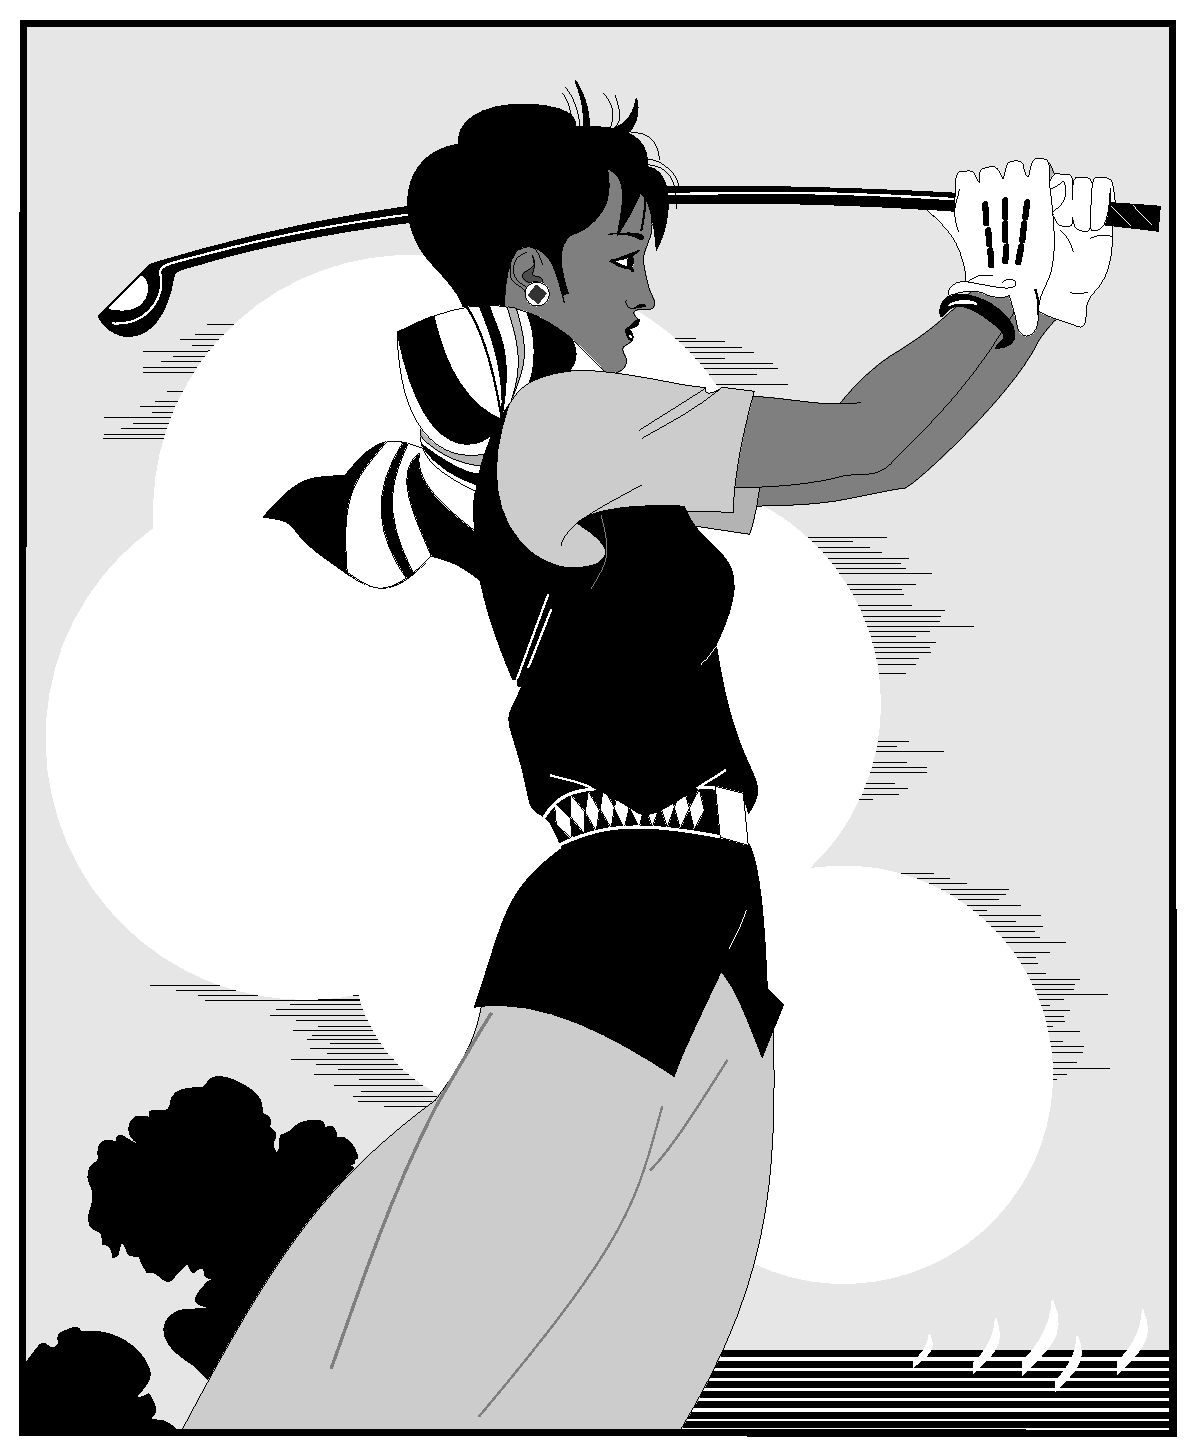
\includegraphics[width = 0.4\textwidth]{golfer}
\caption{打高尔夫球的人,硕士论文要求只用汉语}
\label{fig:bm}
\end{figure}

\subsection{并排图和子图}[Abreast-picture and Sub-picture example]
\subsubsection{并排图}[Abreast-picture example]

使用并排图时,需要注意对齐方式。默认情况是中部对齐。这里给出中部对齐、顶部对齐
、图片底部对齐三种常见方式。其中,底部对齐方式有一个很巧妙的方式,将长度比较小
的图放在左面即可。

\lipsum[2]

\begin{figure}[htbp]
\centering
\begin{minipage}{0.4\textwidth}
\centering
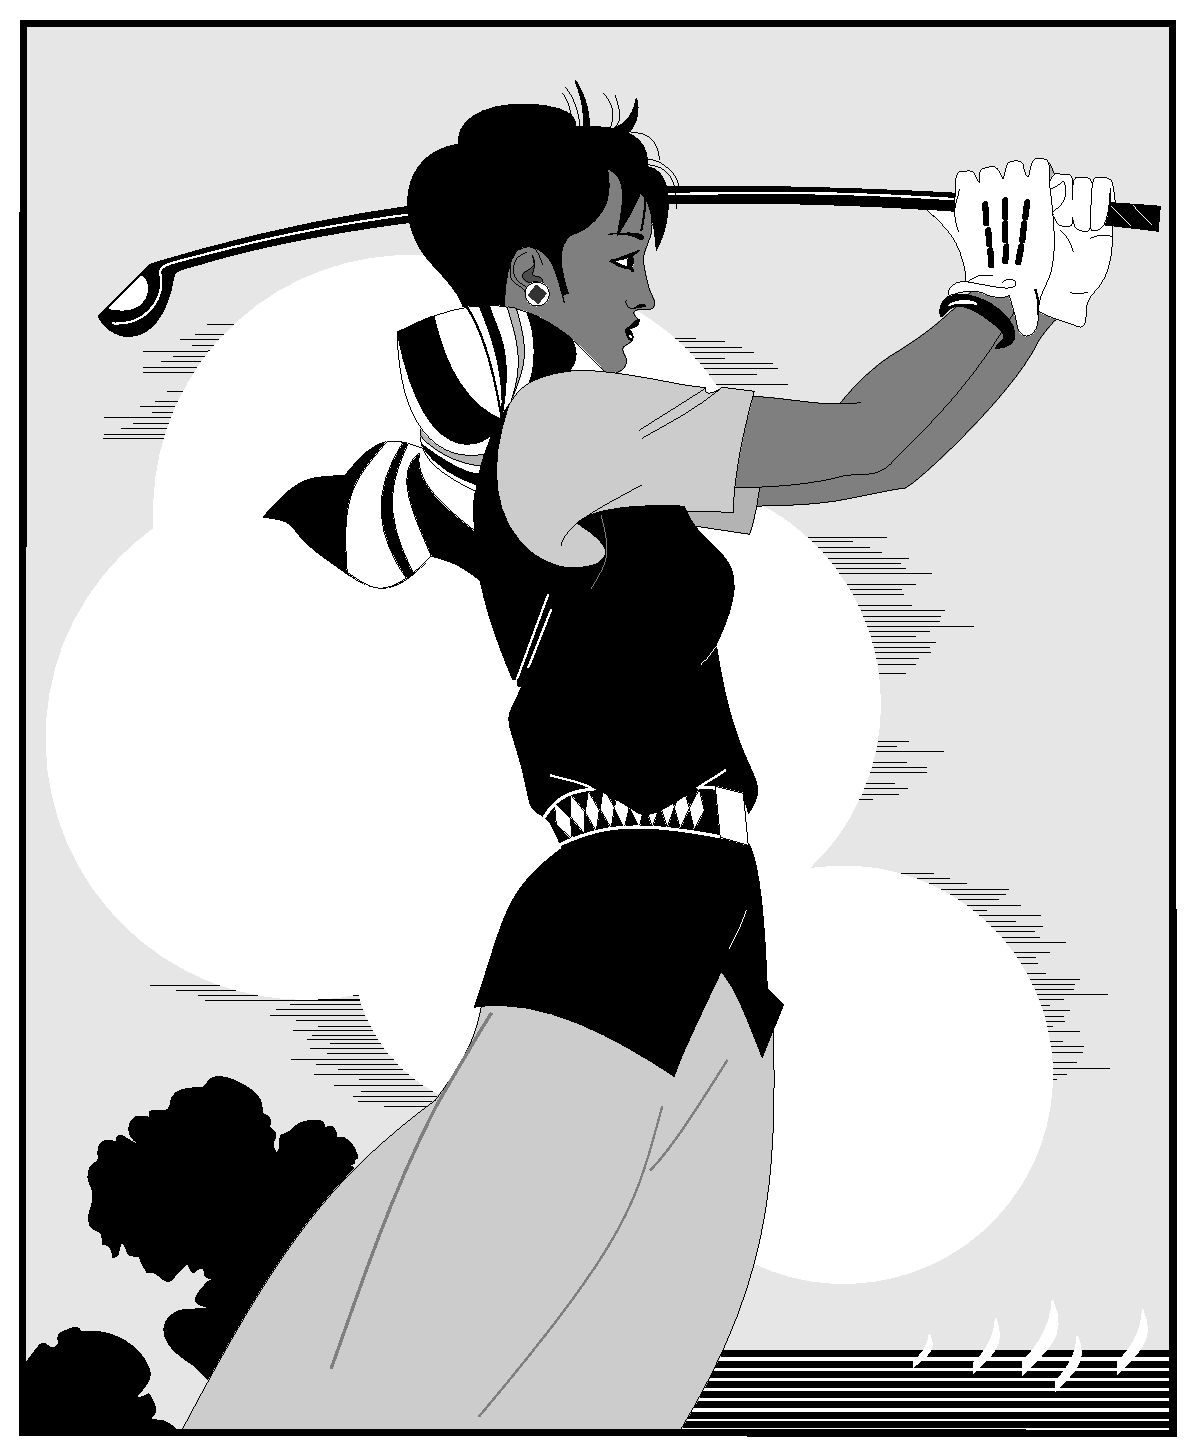
\includegraphics[width=\textwidth]{golfer}
\bicaption[golfer2]{}{打高尔夫球的人}{Fig.$\!$}{The person playing golf}
\end{minipage}
\centering
\begin{minipage}{0.4\textwidth}
\centering
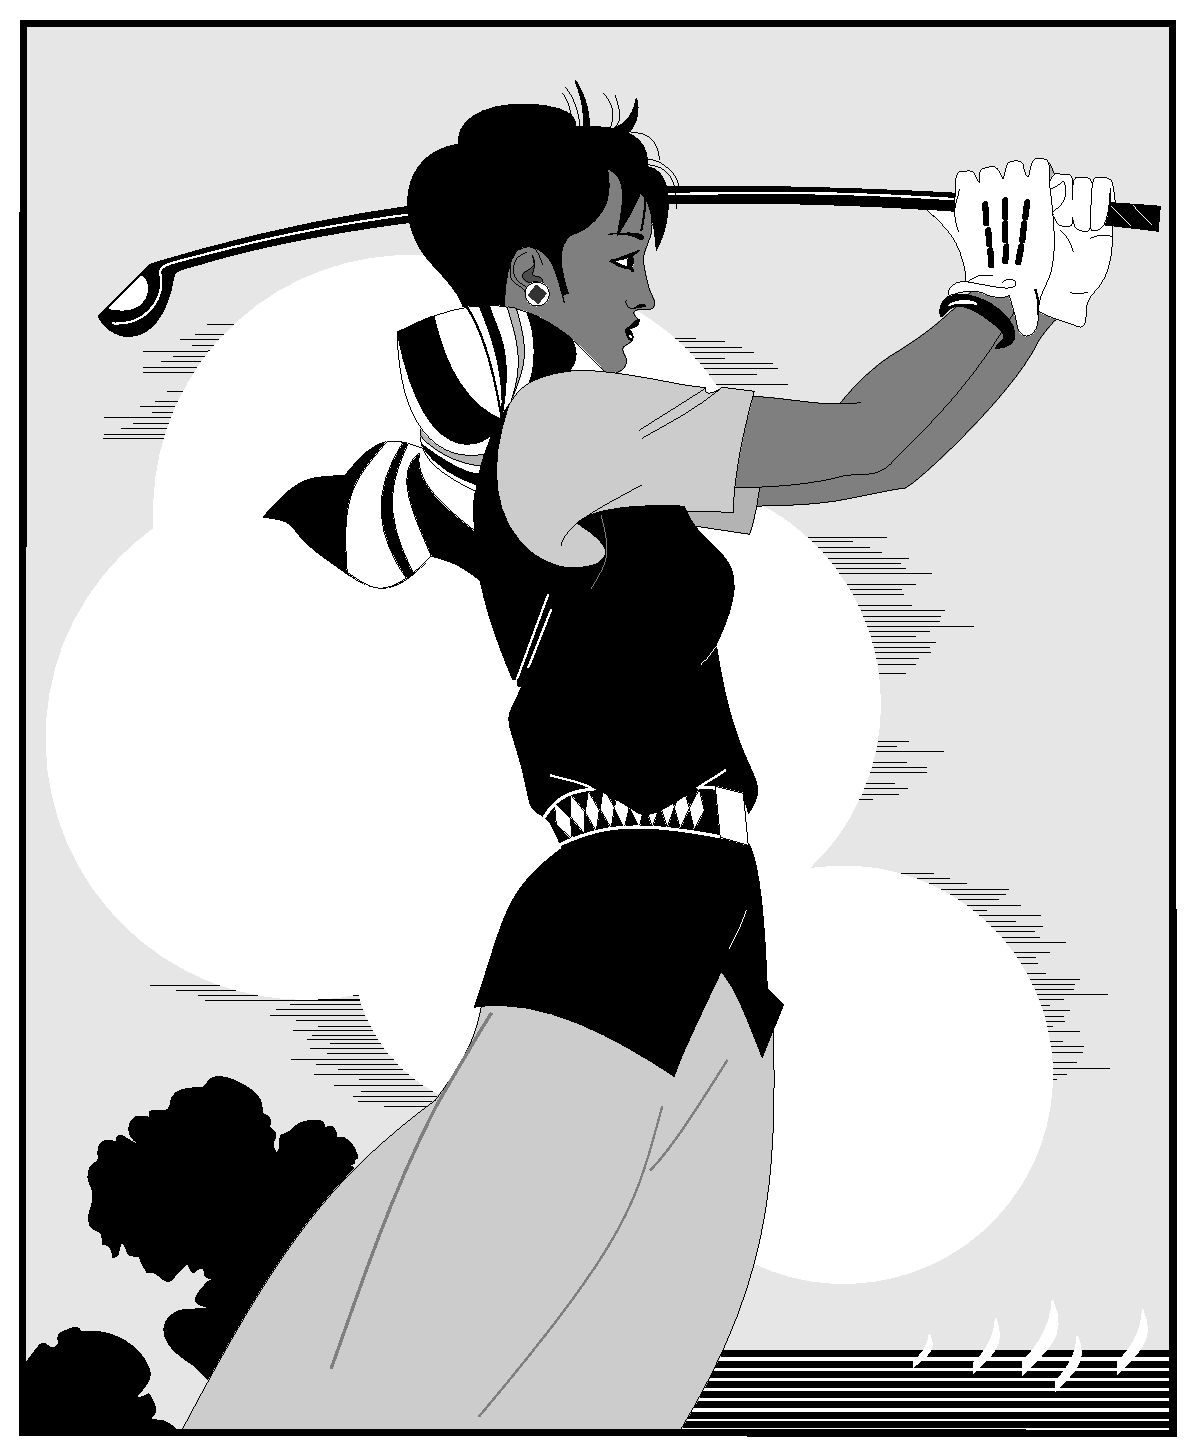
\includegraphics[width=\textwidth]{golfer}
\bicaption[golfer3]{}{打高尔夫球的人。注意,这里默认居中}{Fig.$\!$}{The person playing golf. Please note that, it is vertically center aligned by default.}
\end{minipage}
\end{figure}

\begin{figure}[htbp]
\centering
\begin{minipage}[t]{0.4\textwidth}
\centering
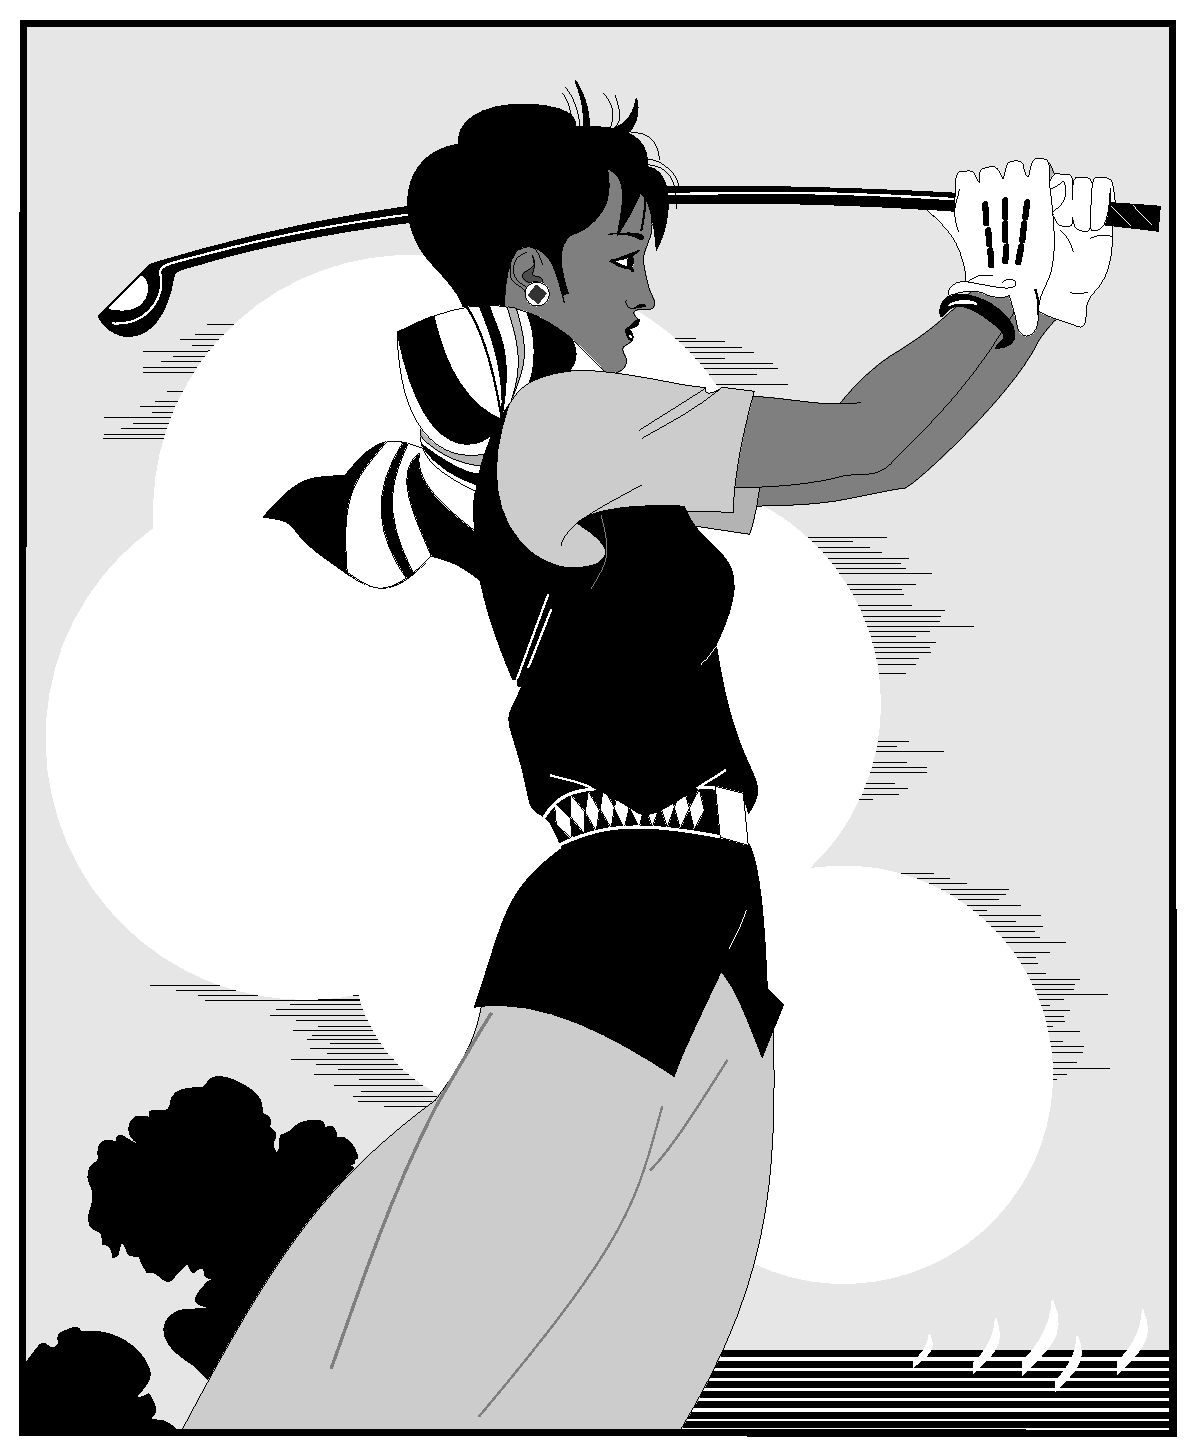
\includegraphics[width=\textwidth]{golfer}
\bicaption[golfer5]{}{打高尔夫球的人}{Fig.$\!$}{The person playing golf}
\end{minipage}
\centering
\begin{minipage}[t]{0.4\textwidth}
\centering
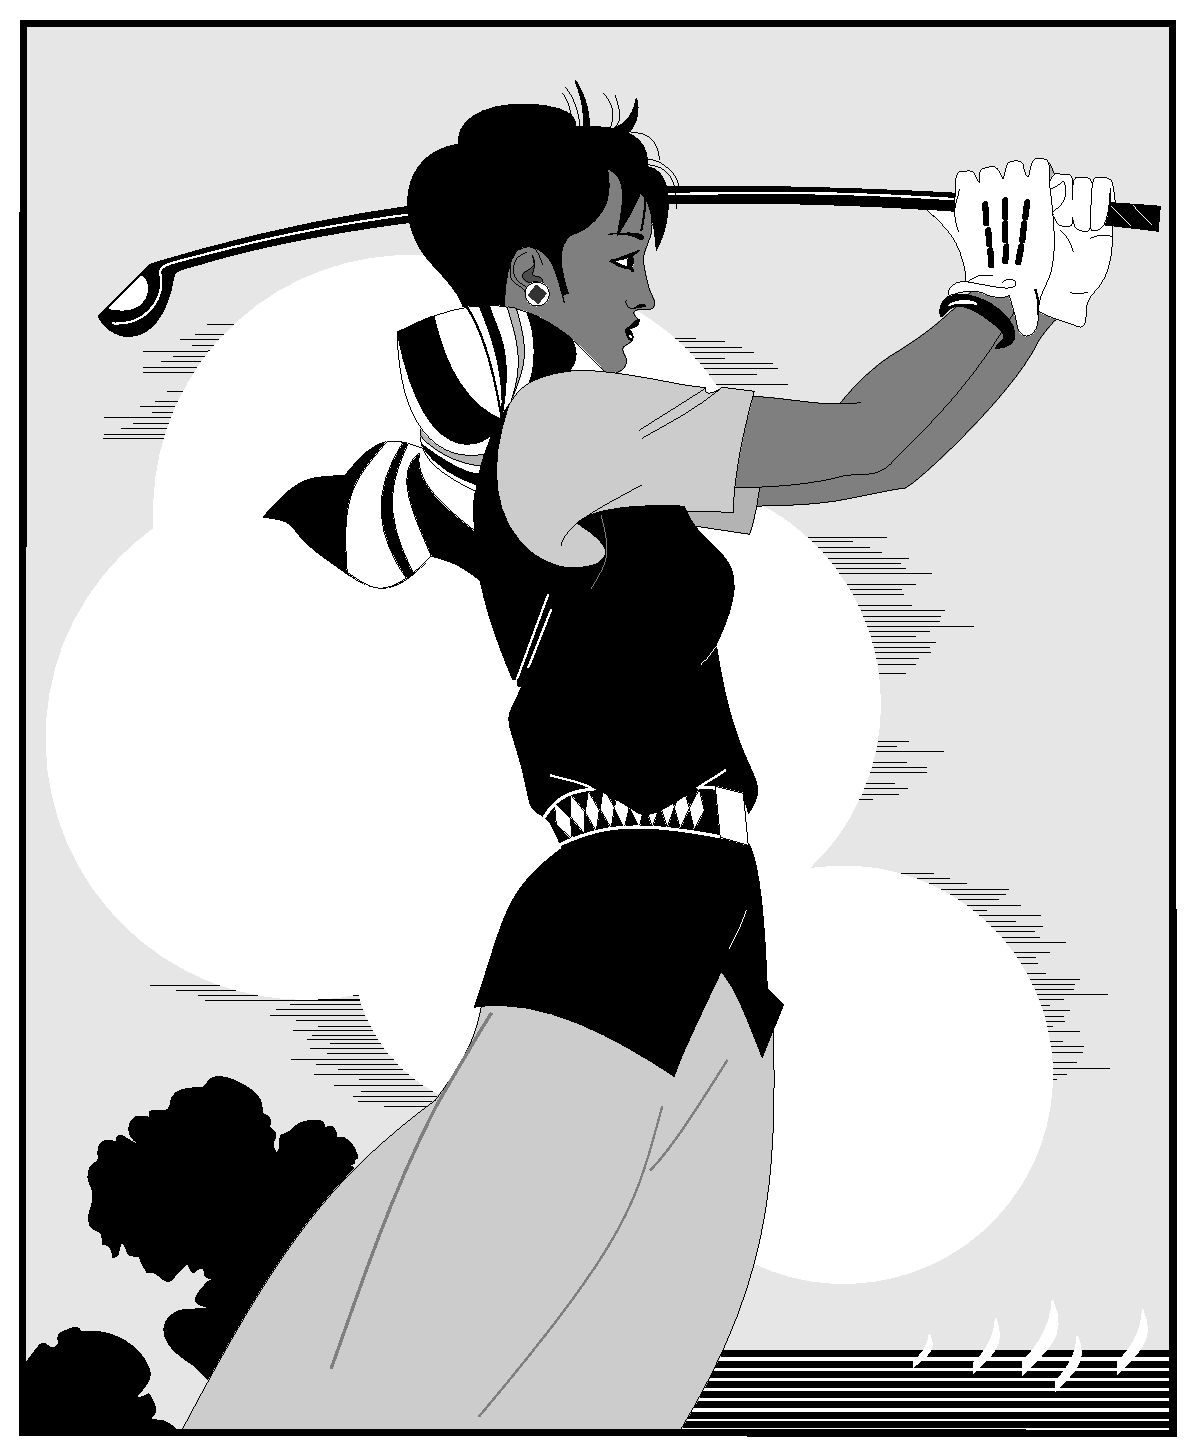
\includegraphics[width=\textwidth]{golfer}
\bicaption[golfer8]{}{打高尔夫球的人。注意,此图是顶部对齐}{Fig.$\!$}{The person playing golf. Please note that, it is vertically top aligned.}
\end{minipage}
\end{figure}

\begin{figure}[htbp]
\centering
\begin{minipage}[t]{0.4\textwidth}
\centering
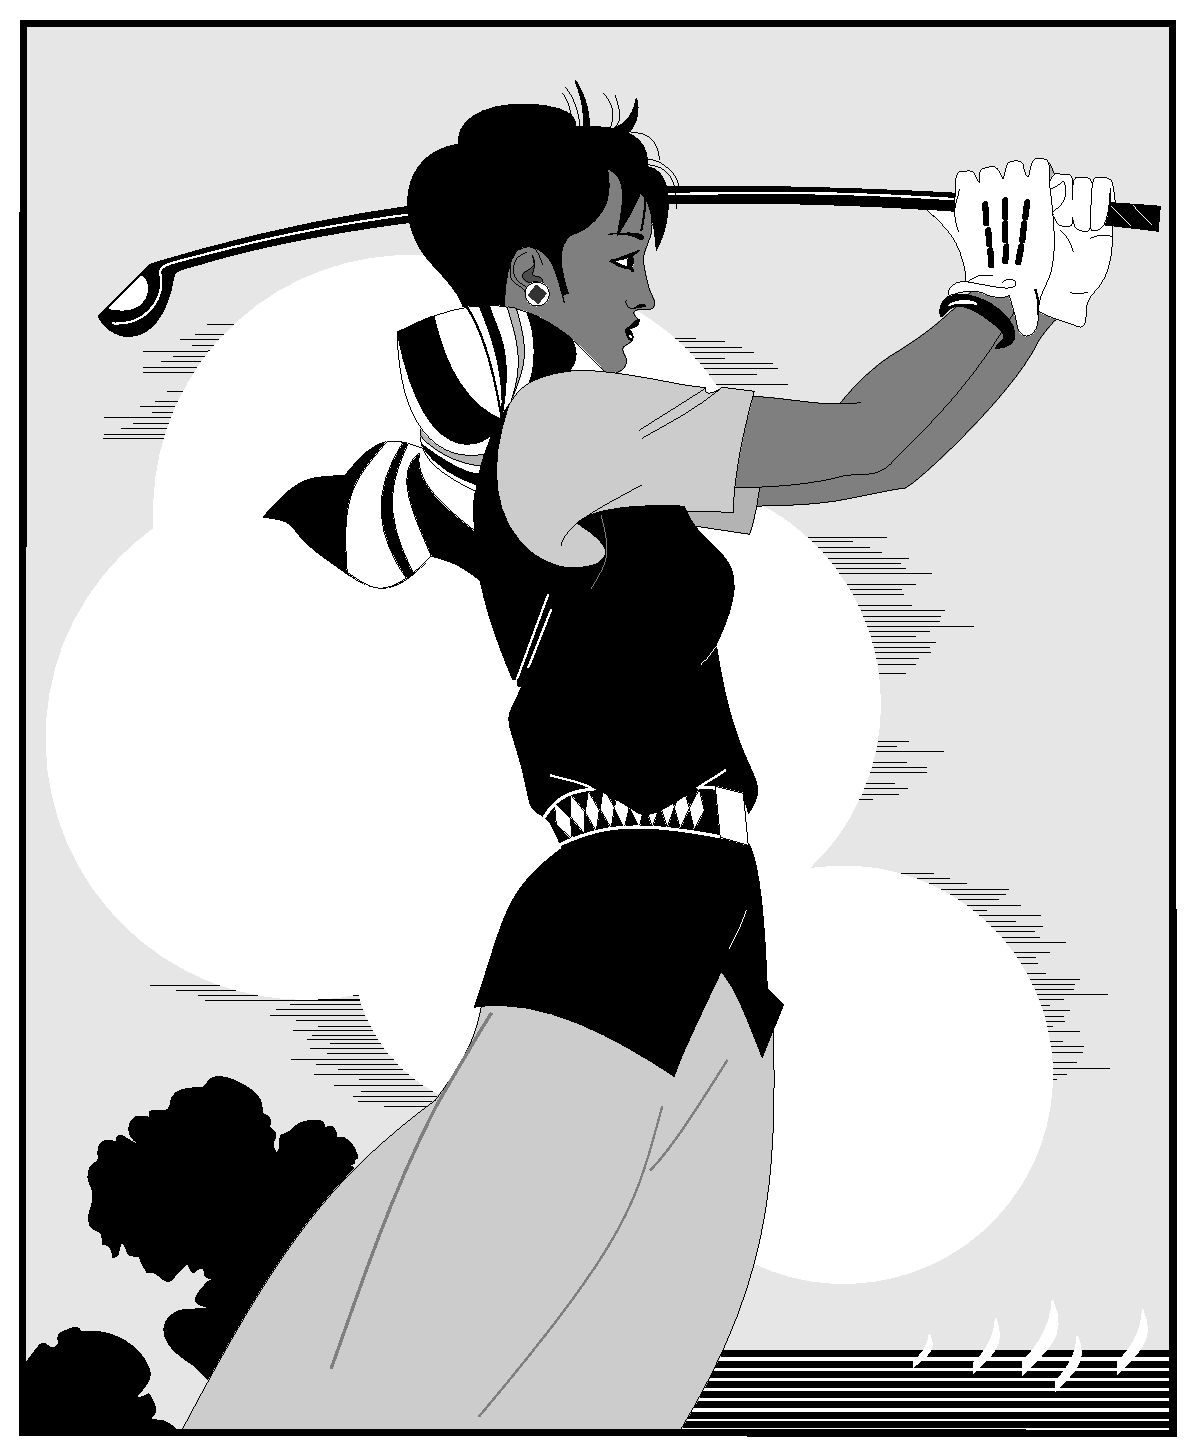
\includegraphics[width=\textwidth,height=\textwidth]{golfer}
\bicaption[golfer9]{}{打高尔夫球的人。注意,此图对齐方式是图片底部对齐}{Fig.$\!$}{The person playing golf. Please note that, it is vertically bottom aligned for figure.}
\end{minipage}
\centering
\begin{minipage}[t]{0.4\textwidth}
\centering
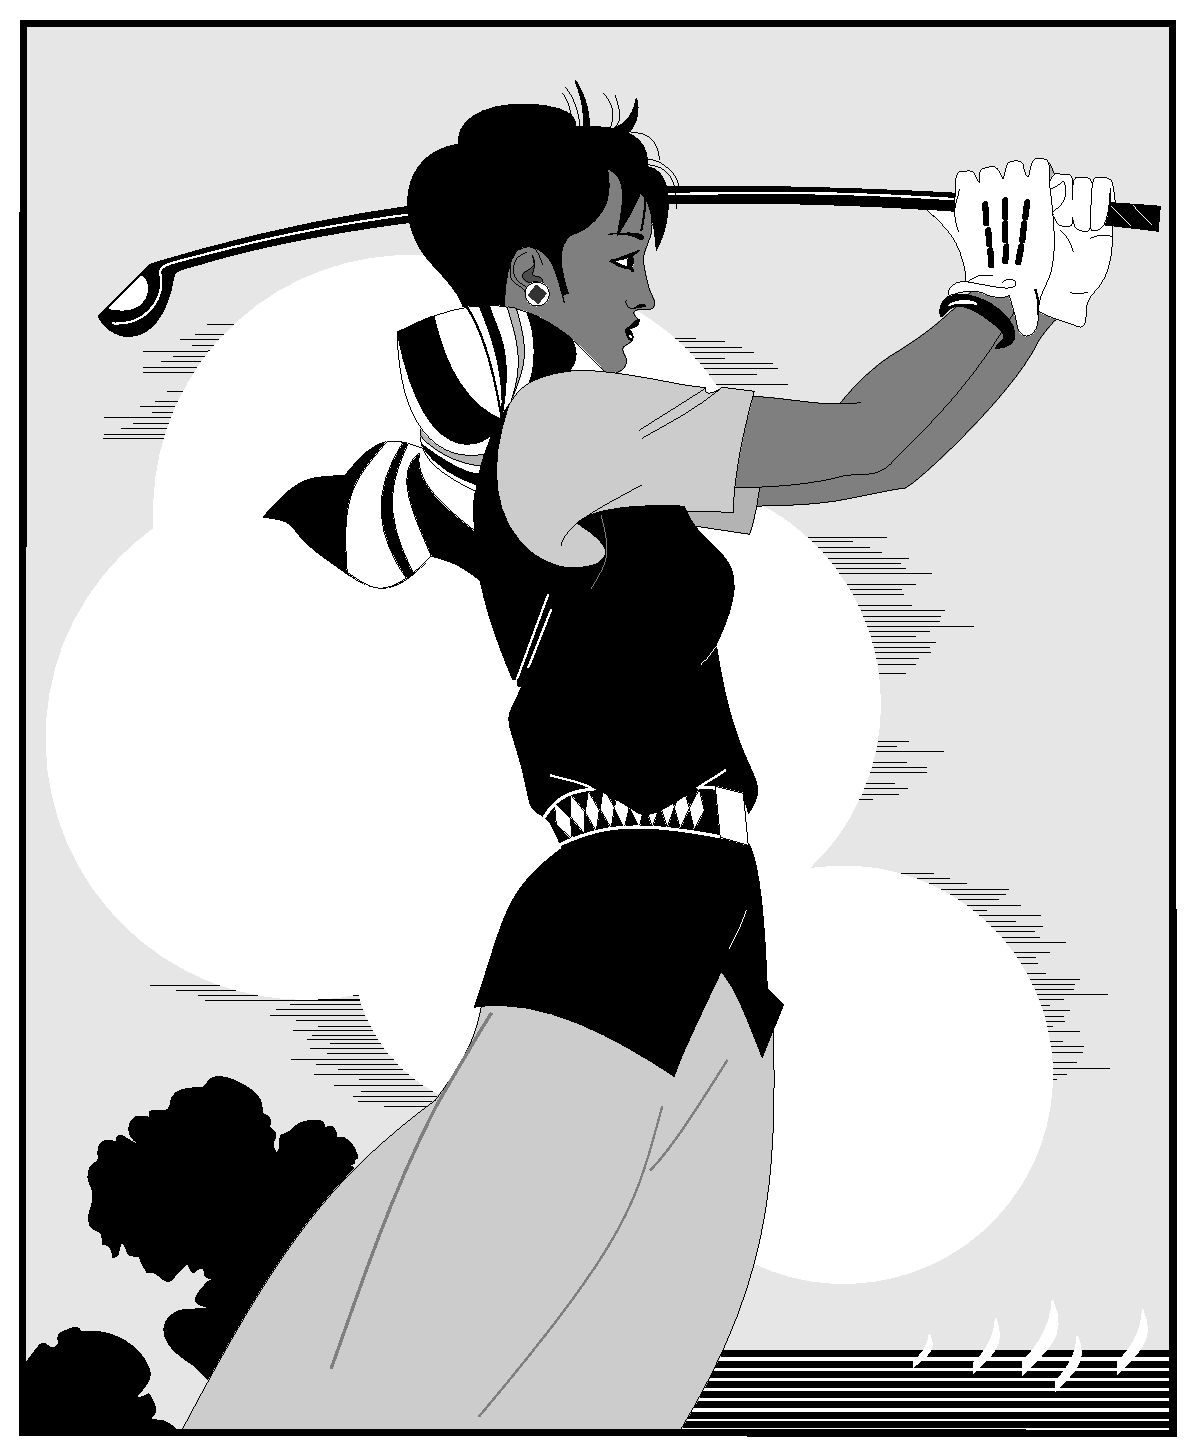
\includegraphics[width=\textwidth]{golfer}
\bicaption[golfer6]{}{打高尔夫球的人}{Fig.$\!$}{The person playing golf}
\end{minipage}
\end{figure}

\subsubsection{子图}[Sub-picture example]

注意:子图题注也可以只用中文。规范规定“分图题置于分图之下或图题之下”,但没有给出具体的格式要求。
没有要求的另外一个说法就是“无论什么格式都不对”。
所以只有在一个图中有标注“a),b)”,无法使用\cs{subfigure}的情况下,使用最后一个图例中的格式设置方法,否则不要使用。
为了应对“无论什么格式都不对”,这个子图图题使用“minipage”和“description”环境,宽度,对齐方式可以按照个人喜好自由设置,是否使用双语子图图题也可以自由设置。

\lipsum[1-3]

无意义文字,每页底部不要留空白。

\lipsum[4-5]

\begin{figure}[!ht]
\setlength{\subfigcapskip}{-1bp}
\centering
\begin{minipage}{\textwidth}
\centering
\subfigure{\label{golfer41}}\addtocounter{subfigure}{-2}
\subfigure[The person playing golf]{\subfigure[打高尔夫球的人~1]{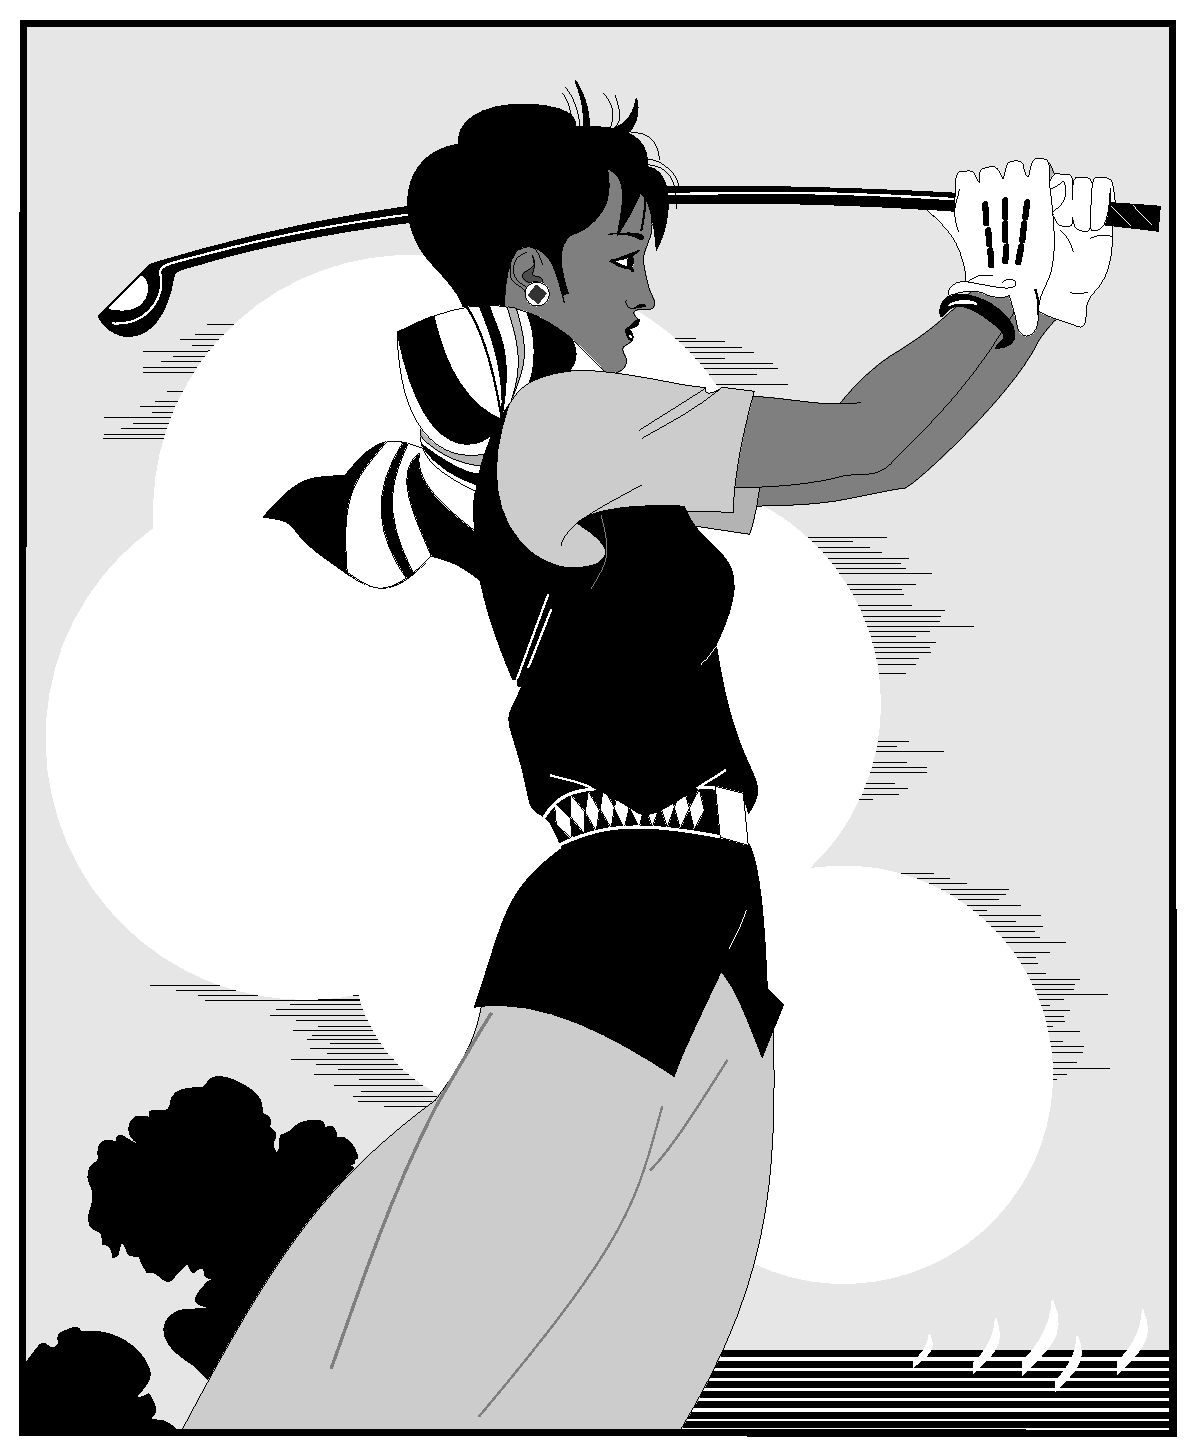
\includegraphics[width=0.4\textwidth]{golfer}}}
\hspace{2em}
\subfigure{\label{golfer42}}\addtocounter{subfigure}{-2}
\subfigure[The person playing golf]{\subfigure[打高尔夫球的人~2]{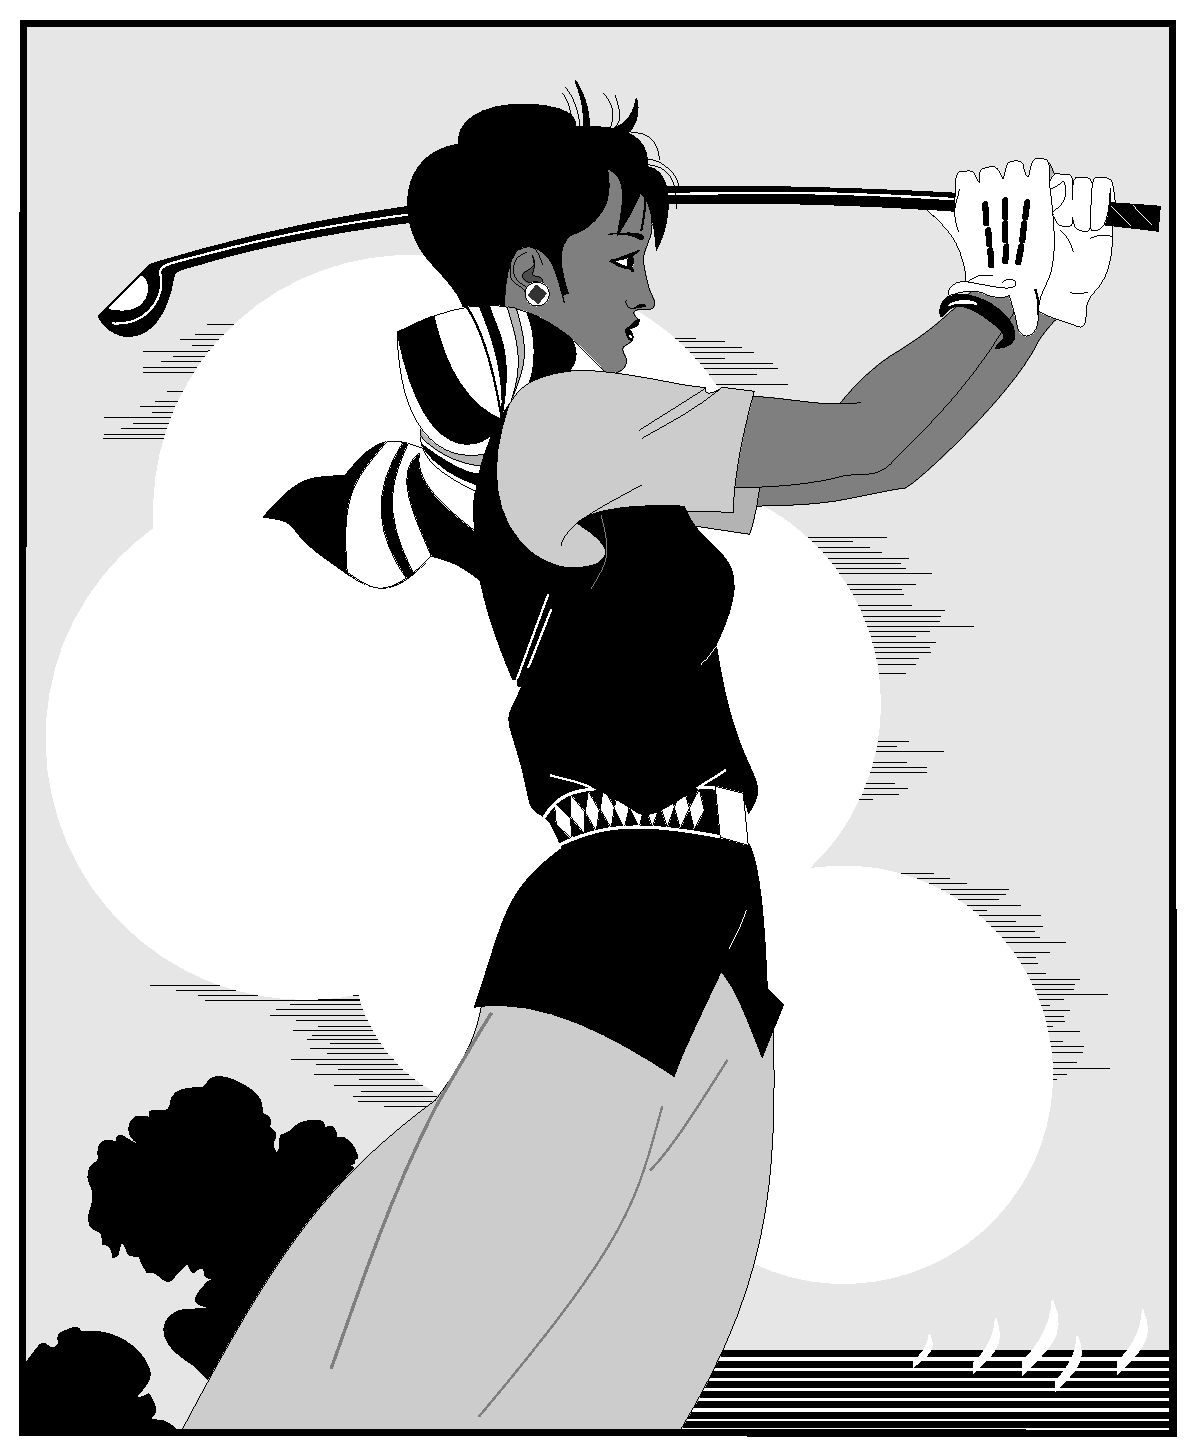
\includegraphics[width=0.4\textwidth]{golfer}}}
\end{minipage}
\centering
\begin{minipage}{\textwidth}
\centering
\subfigure{\label{golfer43}}\addtocounter{subfigure}{-2}
\subfigure[The person playing golf]{\subfigure[打高尔夫球的人~3]{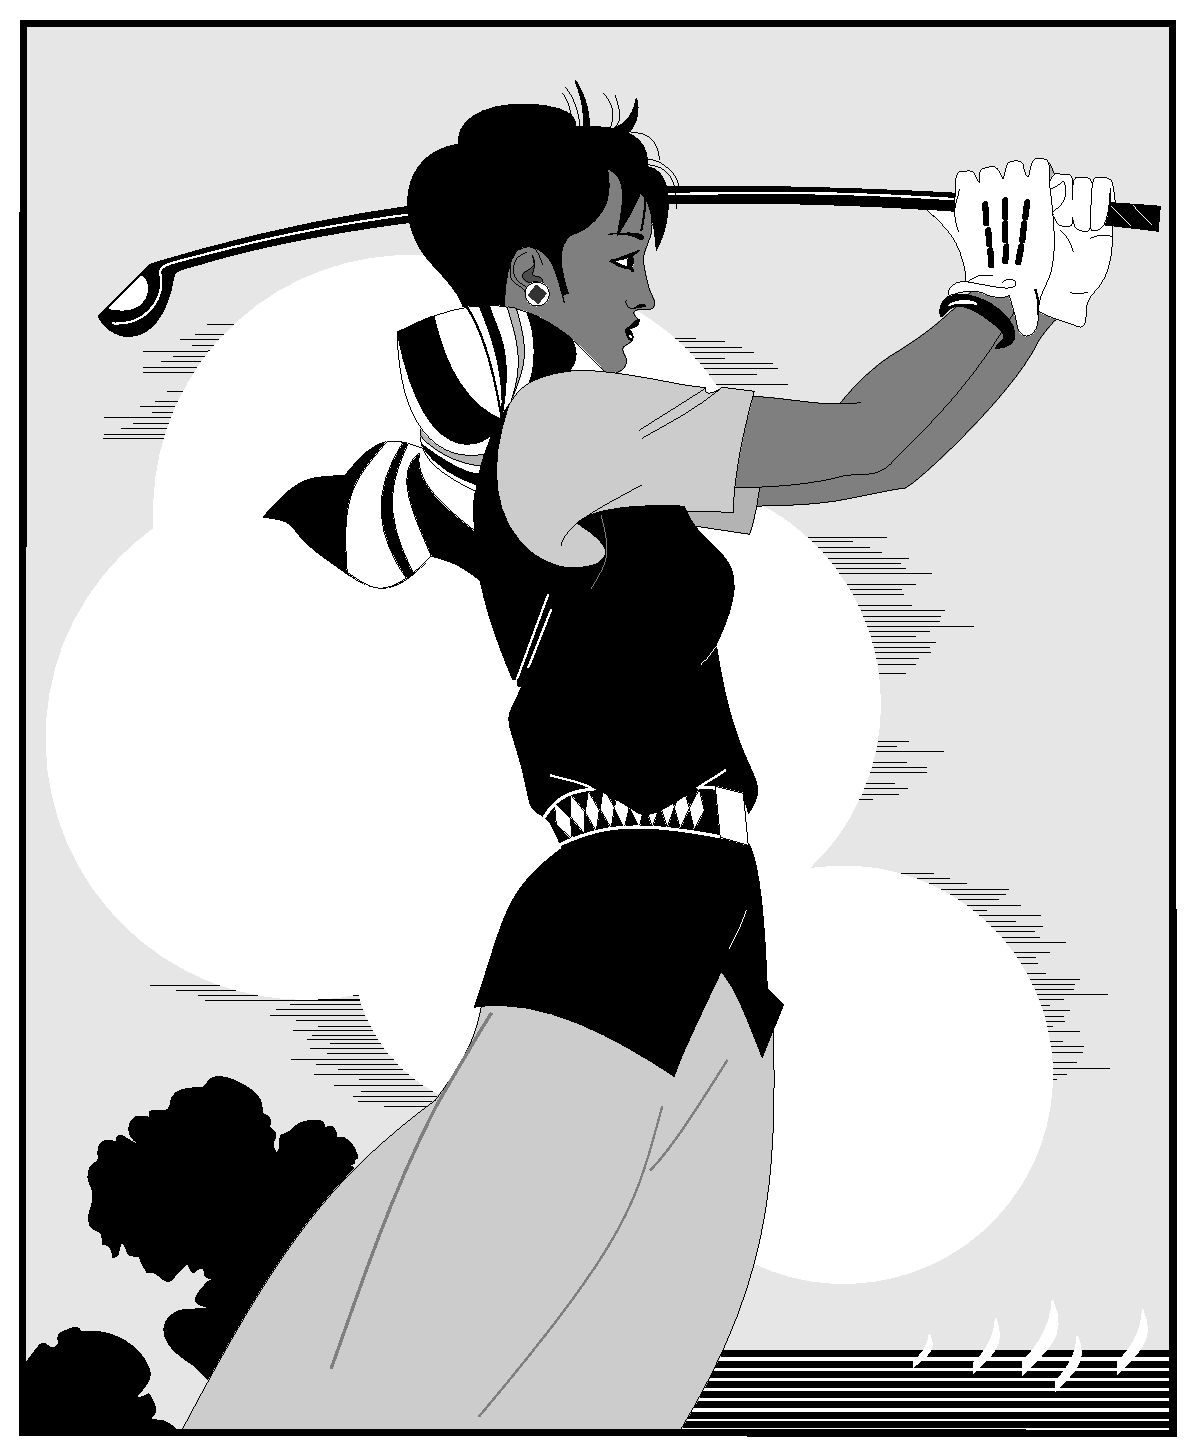
\includegraphics[width=0.4\textwidth]{golfer}}}
\hspace{2em}
\subfigure{\label{golfer44}}\addtocounter{subfigure}{-2}
\subfigure[The person playing golf. Here, 'hang indent' and 'center last line' are not stipulated in the regulation.]{\subfigure[打高尔夫球的人~4。注意,规范中没有明确规定要悬挂缩进、最后一行居中。]{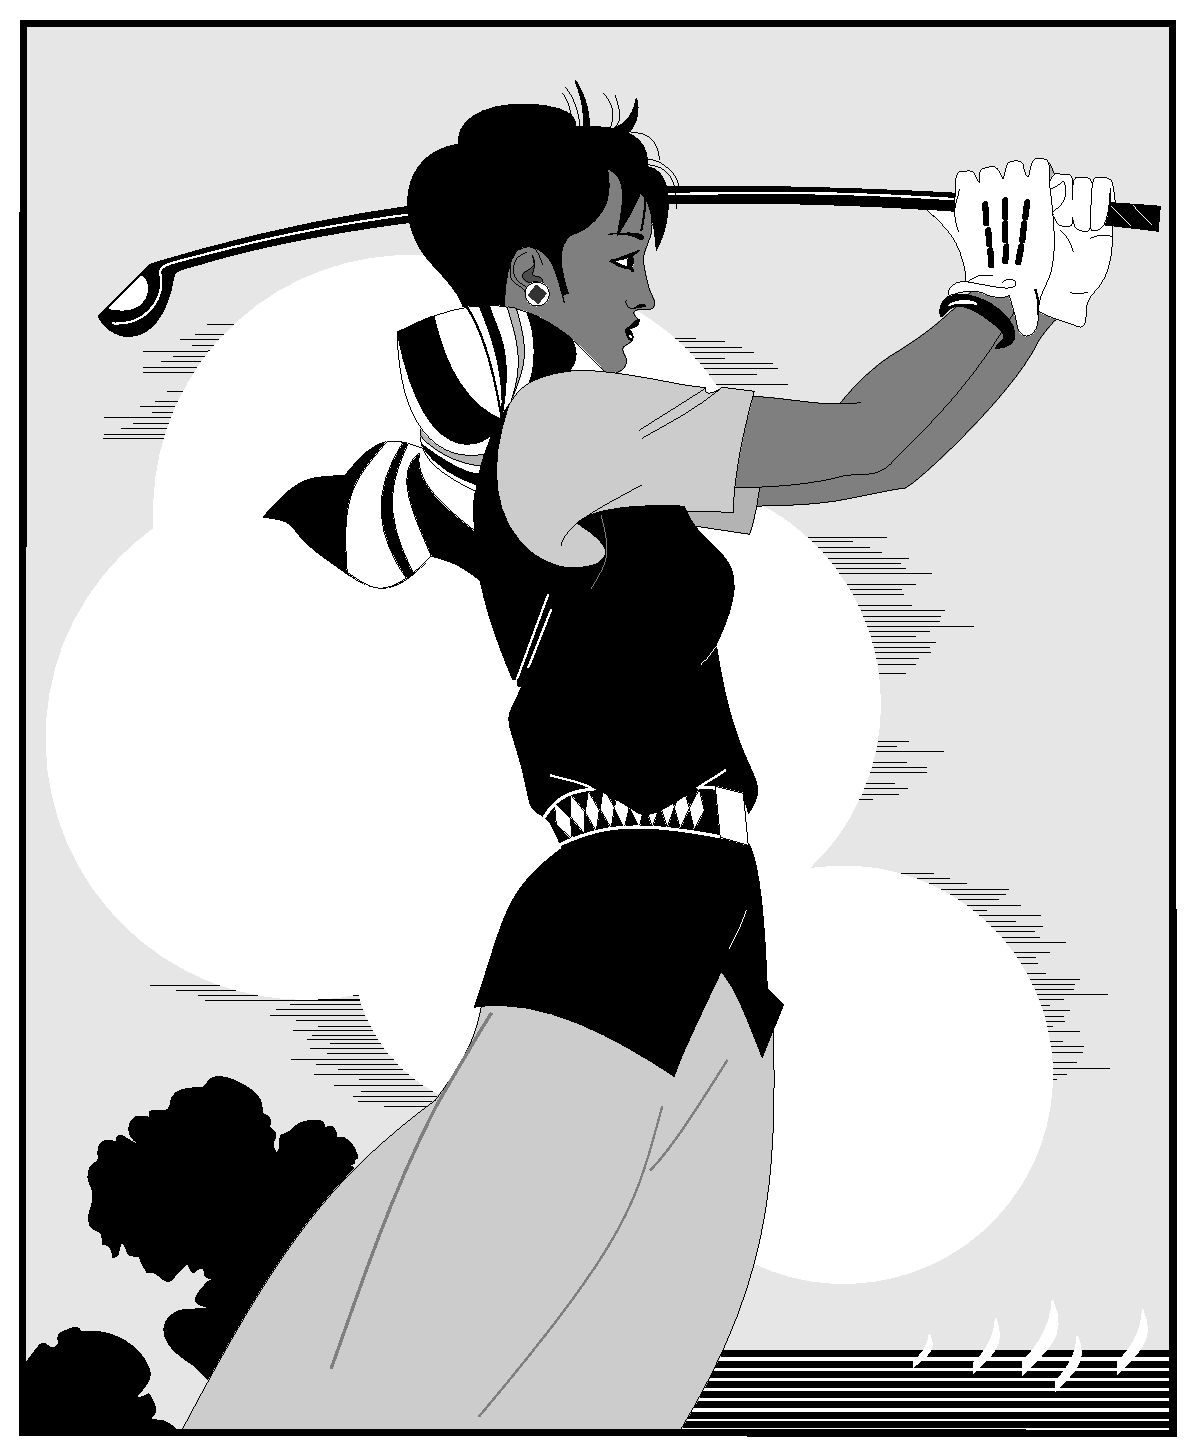
\includegraphics[width=0.4\textwidth]{golfer}}}
\end{minipage}
\vspace{0.2em}
\bicaption[golfer4]{}{打高尔夫球的人}{Fig.$\!$}{The person playing gol}
\end{figure}

\begin{figure}[t]
  \centering
  \begin{minipage}{.7\linewidth}
    \setlength{\subfigcapskip}{-1bp}
    \centering
    \begin{minipage}{\textwidth}
      \centering
      \subfigure{\label{golfer45}}\addtocounter{subfigure}{-2}
      \subfigure[The person playing golf]{\subfigure[打高尔夫球的人~1]{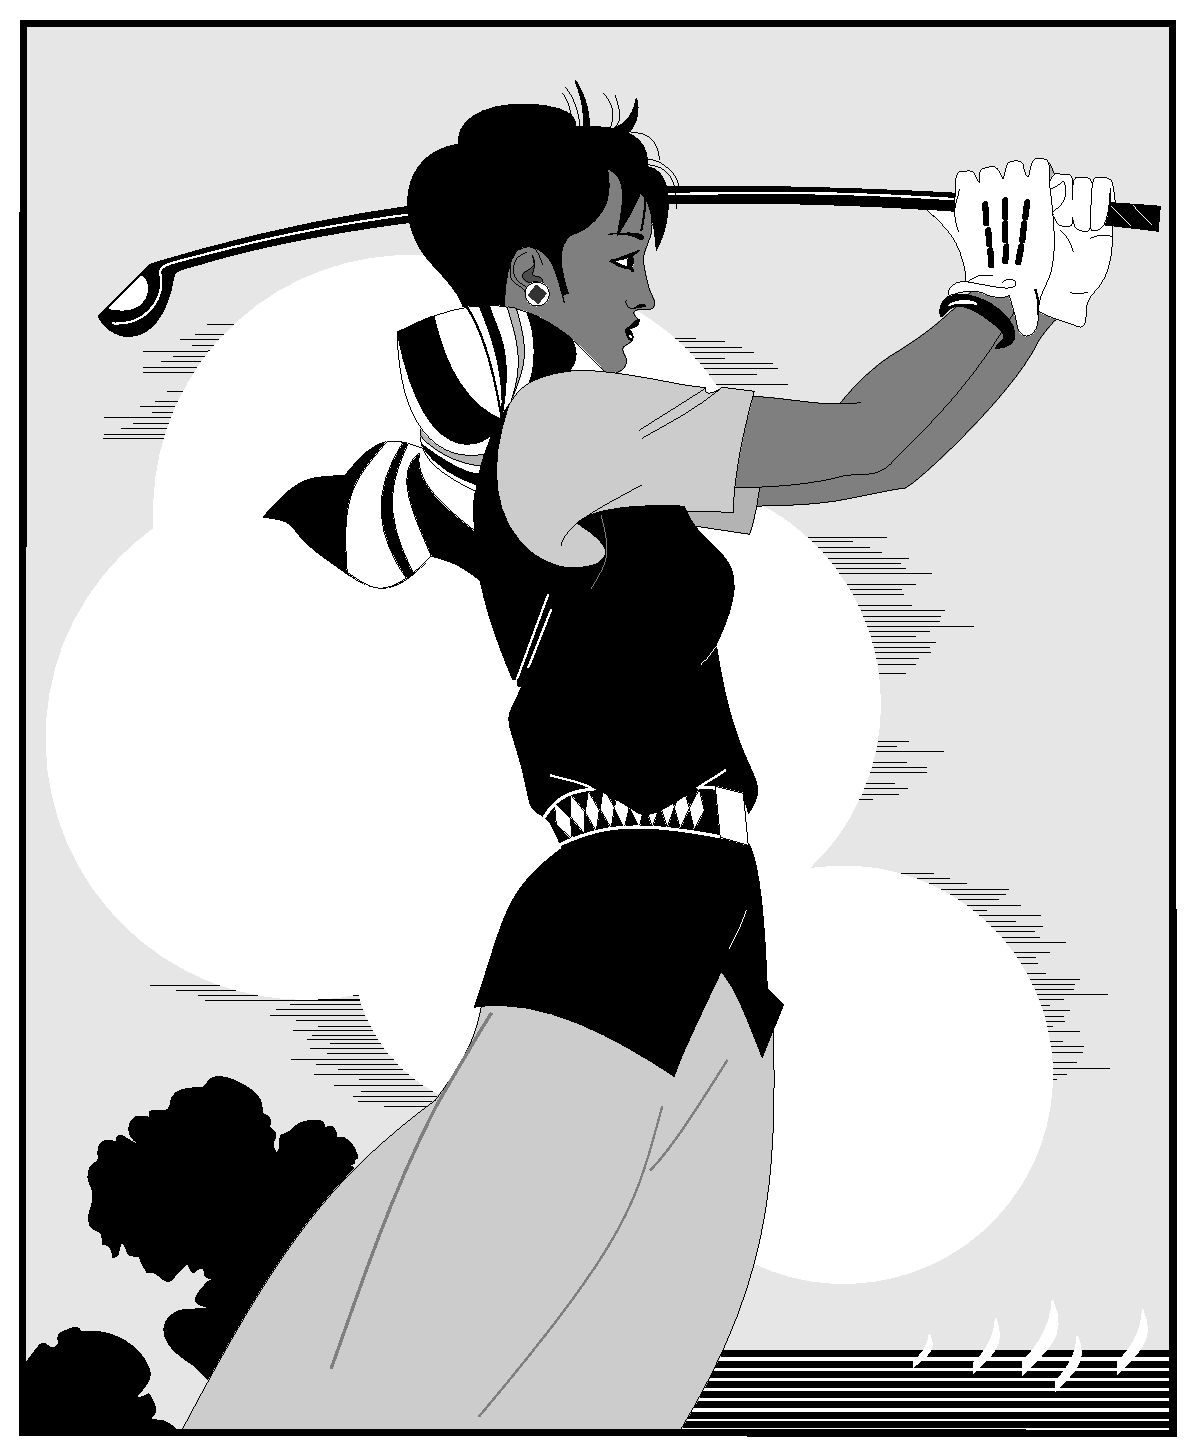
\includegraphics[width=0.4\textwidth]{golfer}}}
      \hspace{4em}
      \subfigure{\label{golfer46}}\addtocounter{subfigure}{-2}
      \subfigure[The person playing golf]{\subfigure[打高尔夫球的人~2]{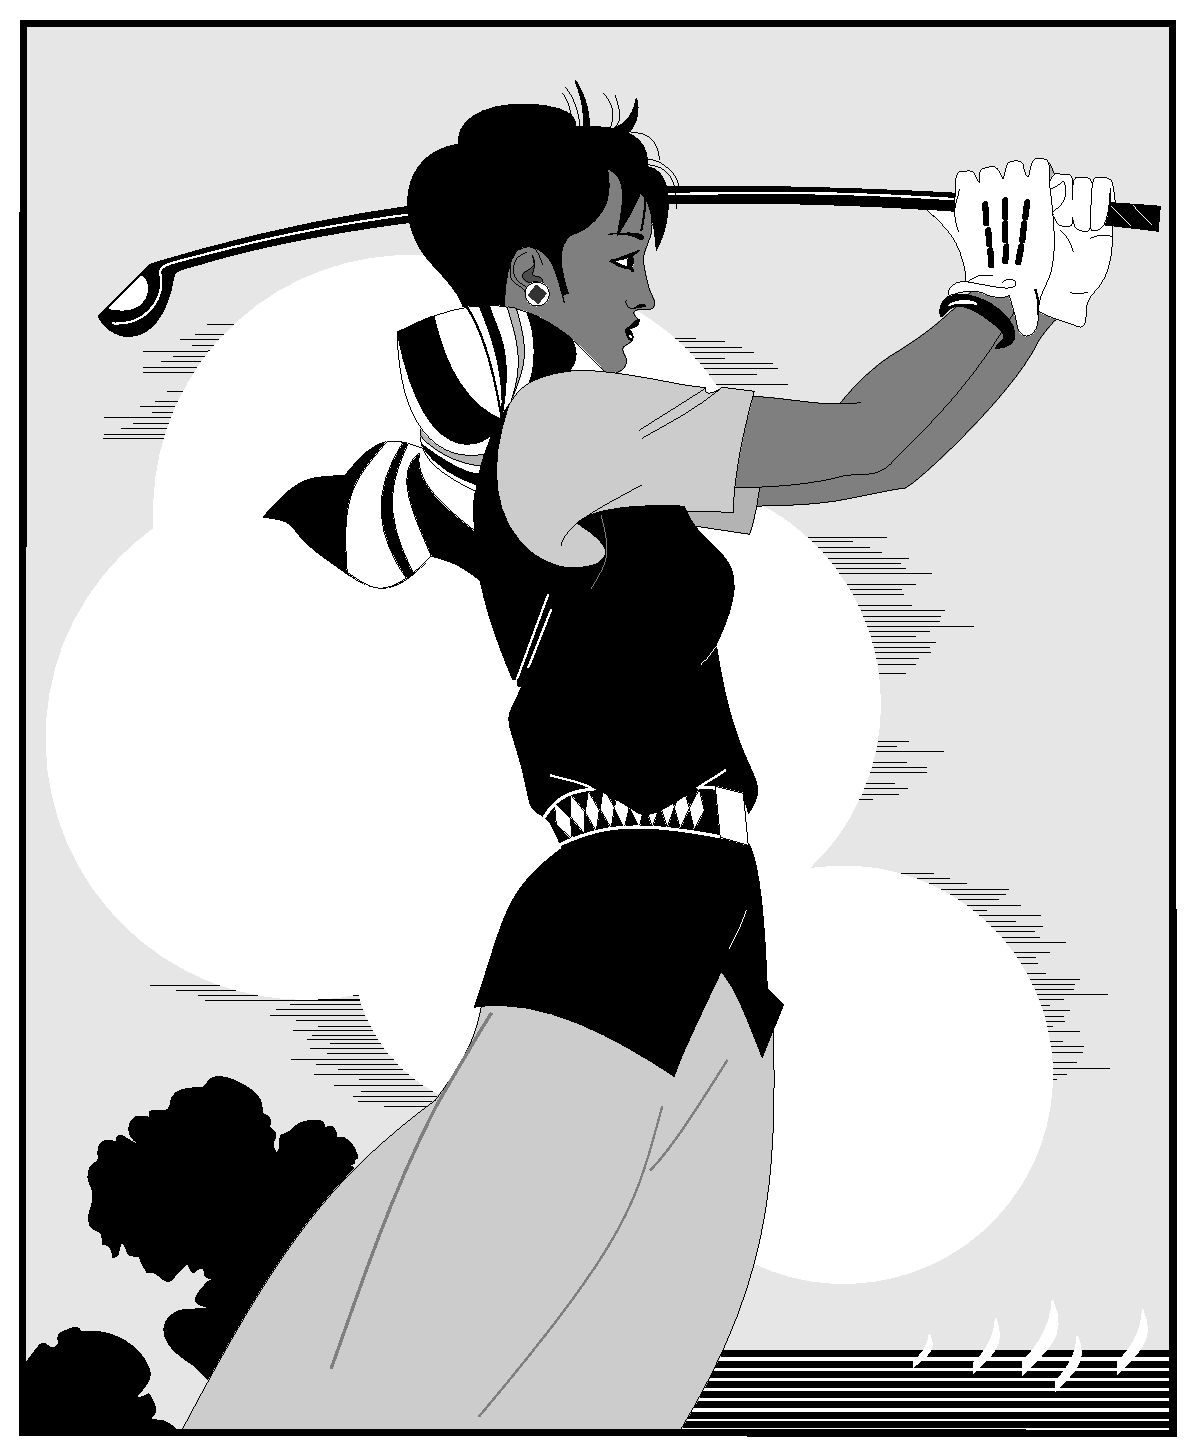
\includegraphics[width=0.4\textwidth]{golfer}}}
    \end{minipage}
    \vskip 0.2em
  \wuhao 注意:这里是中文图注添加位置(我工要求,图注在图题之上)。
    \vspace{0.2em}
\bicaption[golfer47]{}{打高尔夫球的人。注意,此处我工有另外一处要求,子图图题可以位于主图题之下。但由于没有明确说明位于下方具体是什么格式,所以这里不给出举例。}{Fig.$\!$}{The person playing golf. Please note that, although it is appropriate to put subfigures' captions under this caption as stipulated in regulation, but its format is not clearly stated.}
  \end{minipage}
\end{figure}

\begin{figure}[t]
\centering
\begin{tikzpicture}
	\node[anchor=south west,inner sep=0] (image) at (0,0) {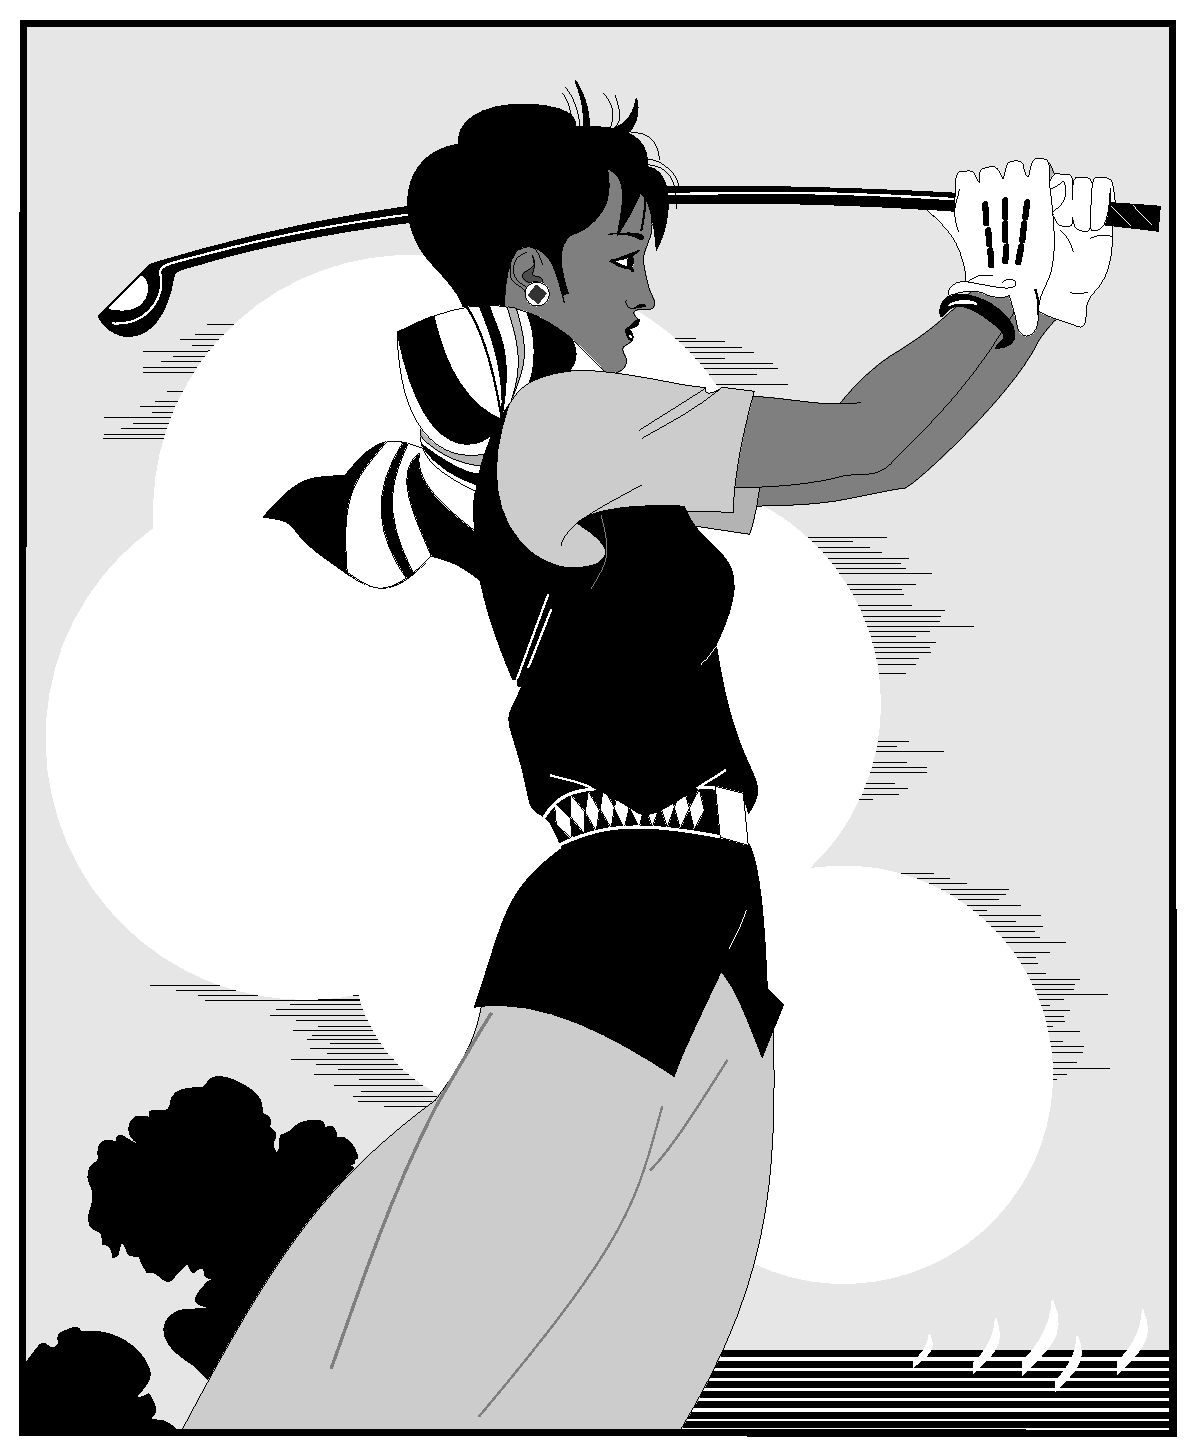
\includegraphics[width=0.3\textwidth]{golfer}};
	\begin{scope}[x={(image.south east)},y={(image.north west)}]
		\node at (0.3,0.5) {a)};
		\node at (0.8,0.2) {b)};
	\end{scope}
\end{tikzpicture}
\bicaption[golfer0]{}{打高尔夫球球的人(博士论文双语题注)}{Fig.$\!$}{The person playing golf (Doctoral thesis)}
\vskip -0.4em
 \hspace{2em}
\begin{minipage}[t]{0.3\textwidth}
\wuhao \setlist[description]{font=\normalfont}
	\begin{description}
		\item[(a)]子图图题
	\end{description}
 \end{minipage}
 \hspace{2em}
 \begin{minipage}[t]{0.3\textwidth}
\wuhao \setlist[description]{font=\normalfont}
	\begin{description}
		\item[(b)]子图图题
		\item[(b)]Subfigure caption
	\end{description}
\end{minipage}
\end{figure}


\begin{figure}[!ht]
	\centering
	\begin{sideways}
		\begin{minipage}{\textheight}
			\centering
			\fbox{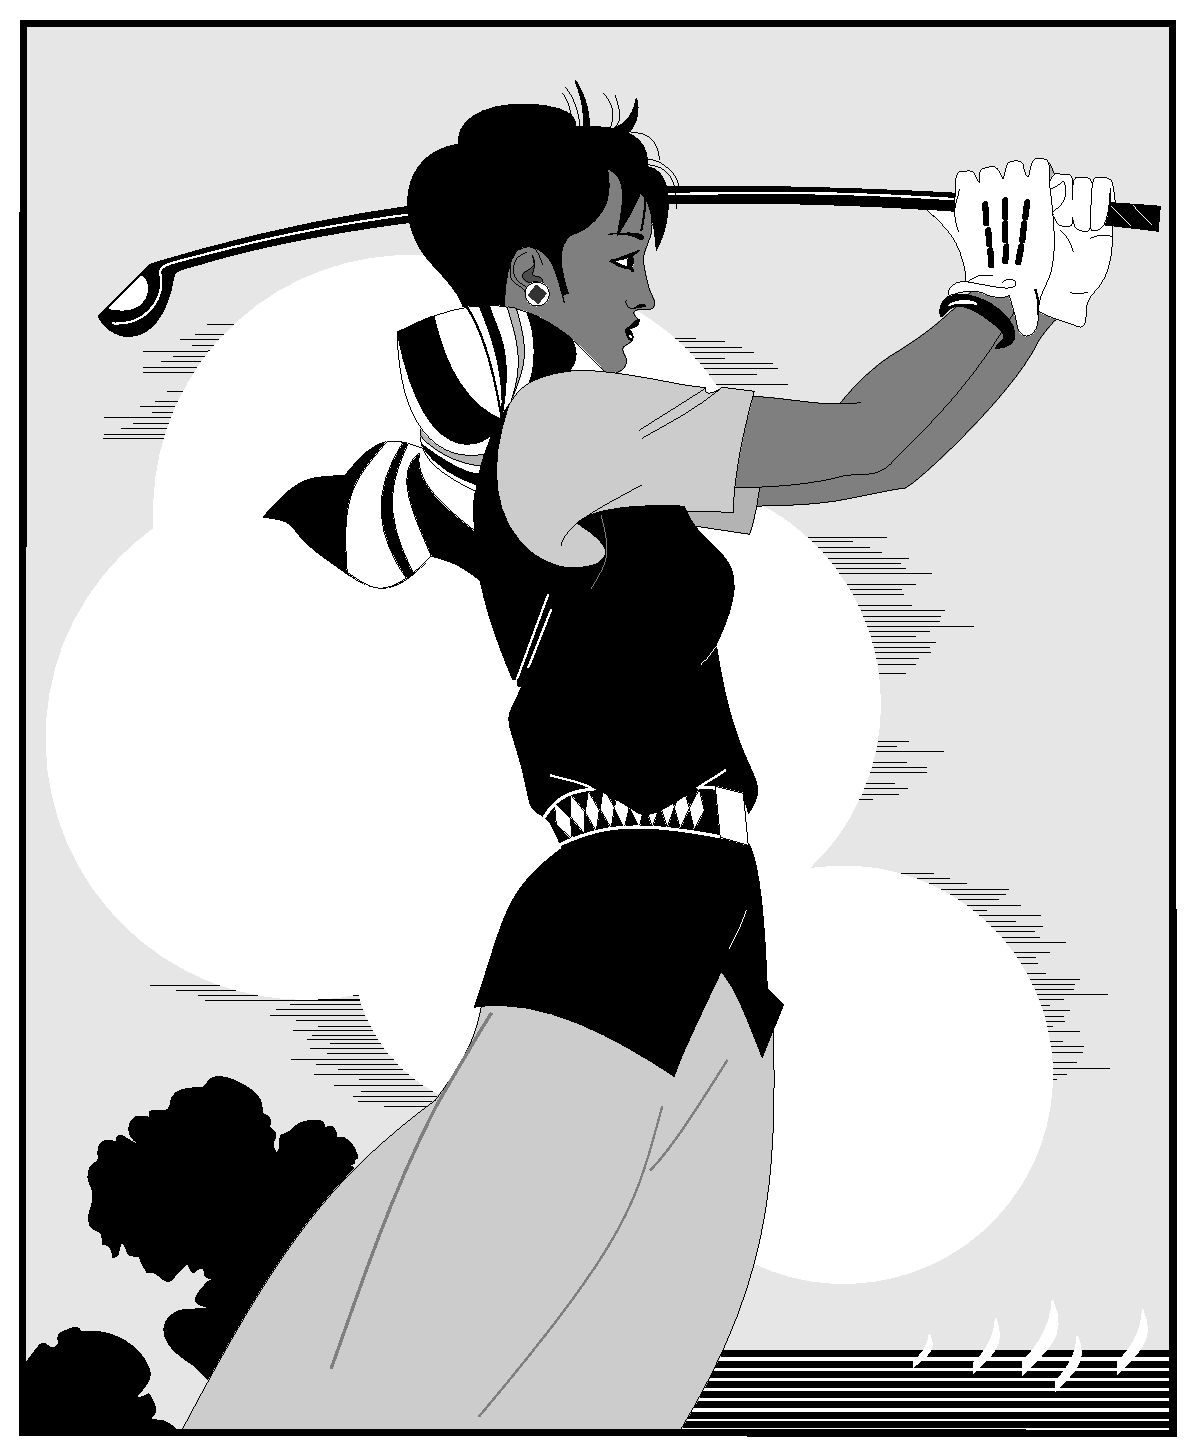
\includegraphics[width=0.2\textwidth]{golfer}}
			\fbox{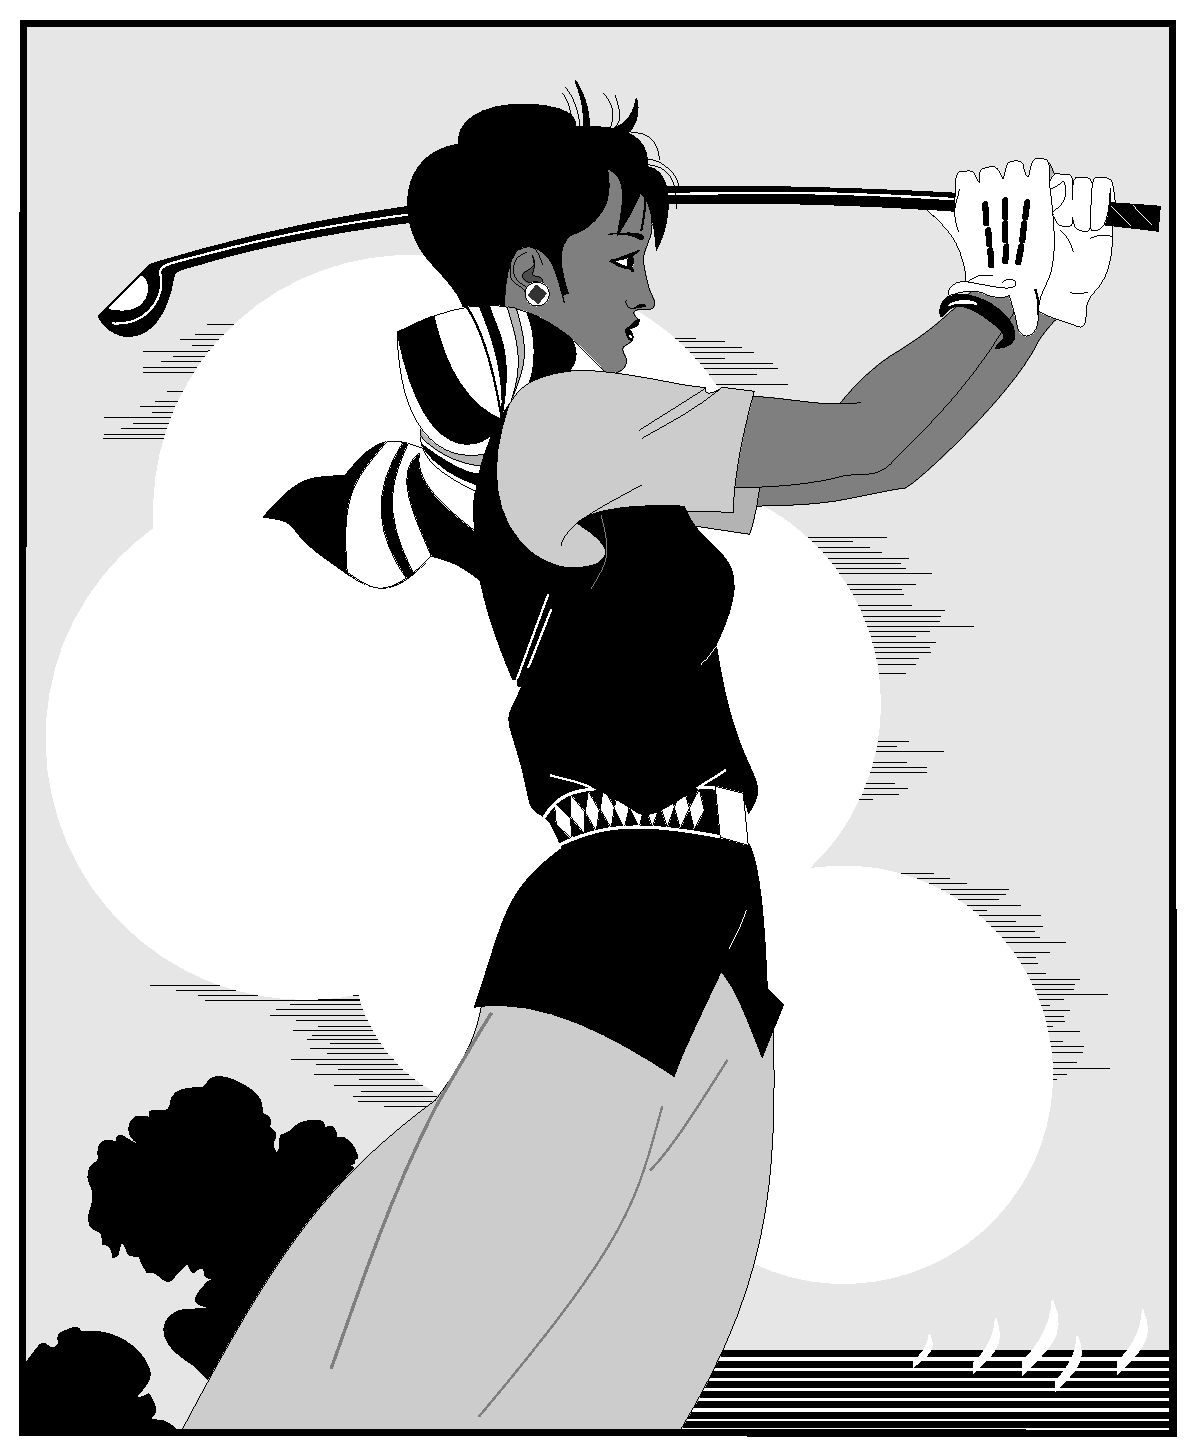
\includegraphics[width=0.2\textwidth]{golfer}}
			\fbox{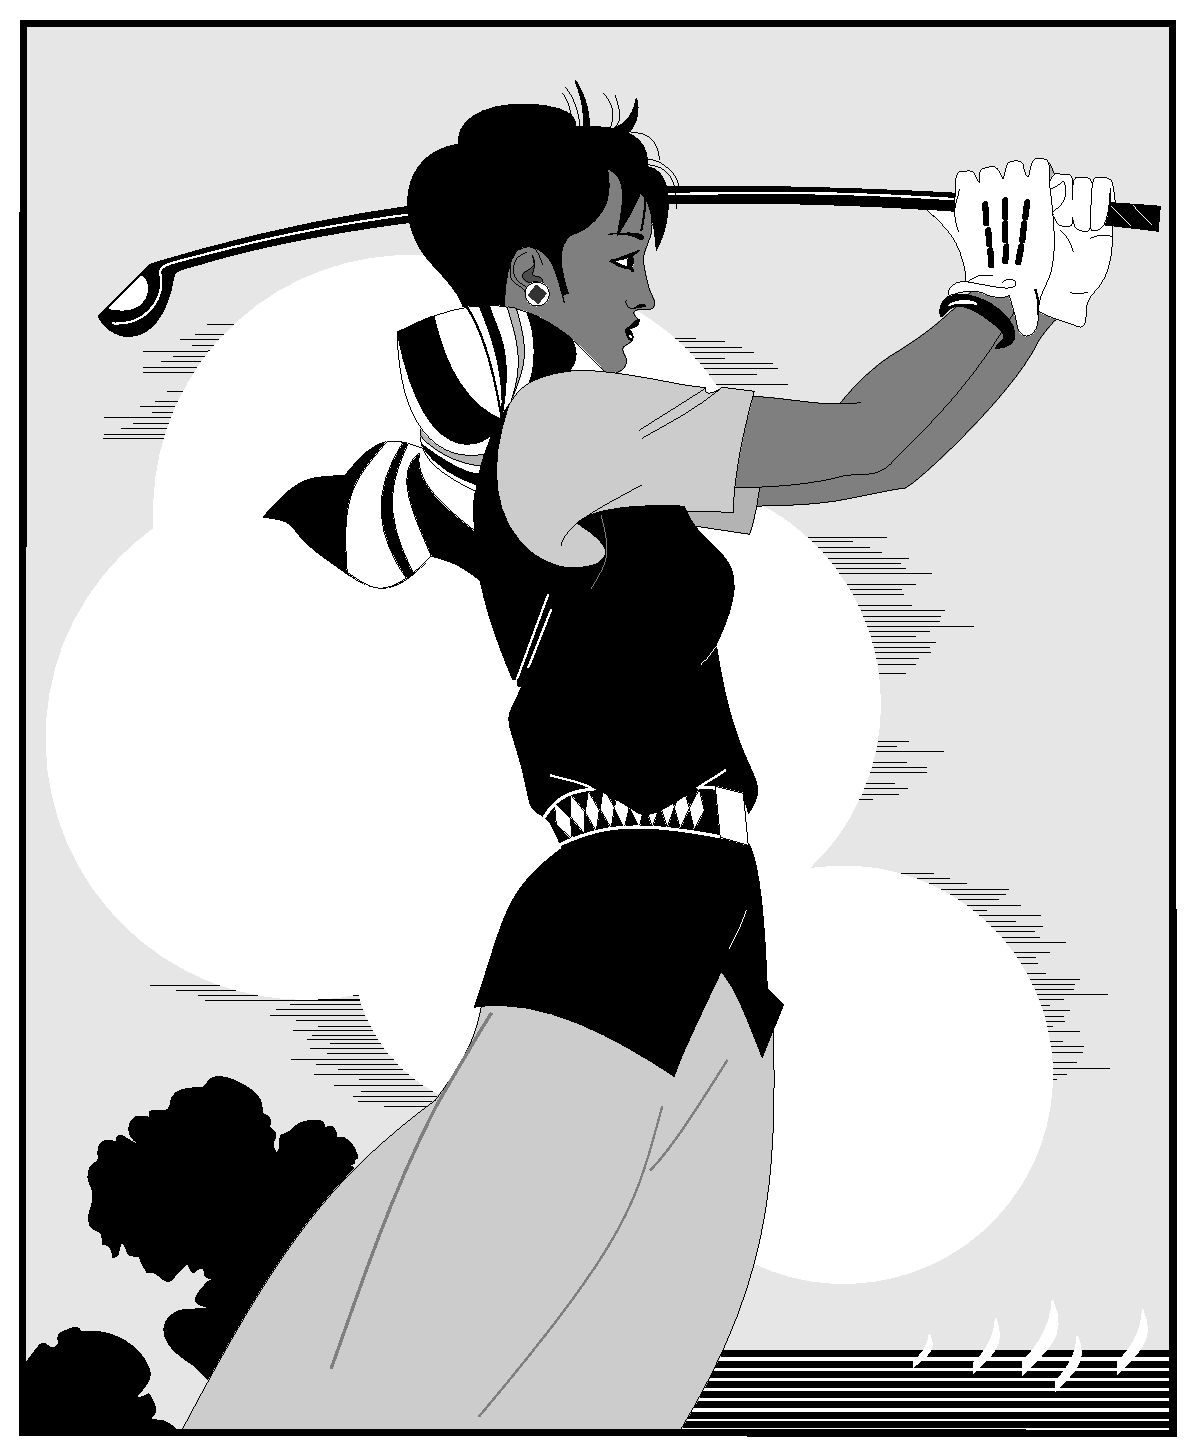
\includegraphics[width=0.2\textwidth]{golfer}}
			\fbox{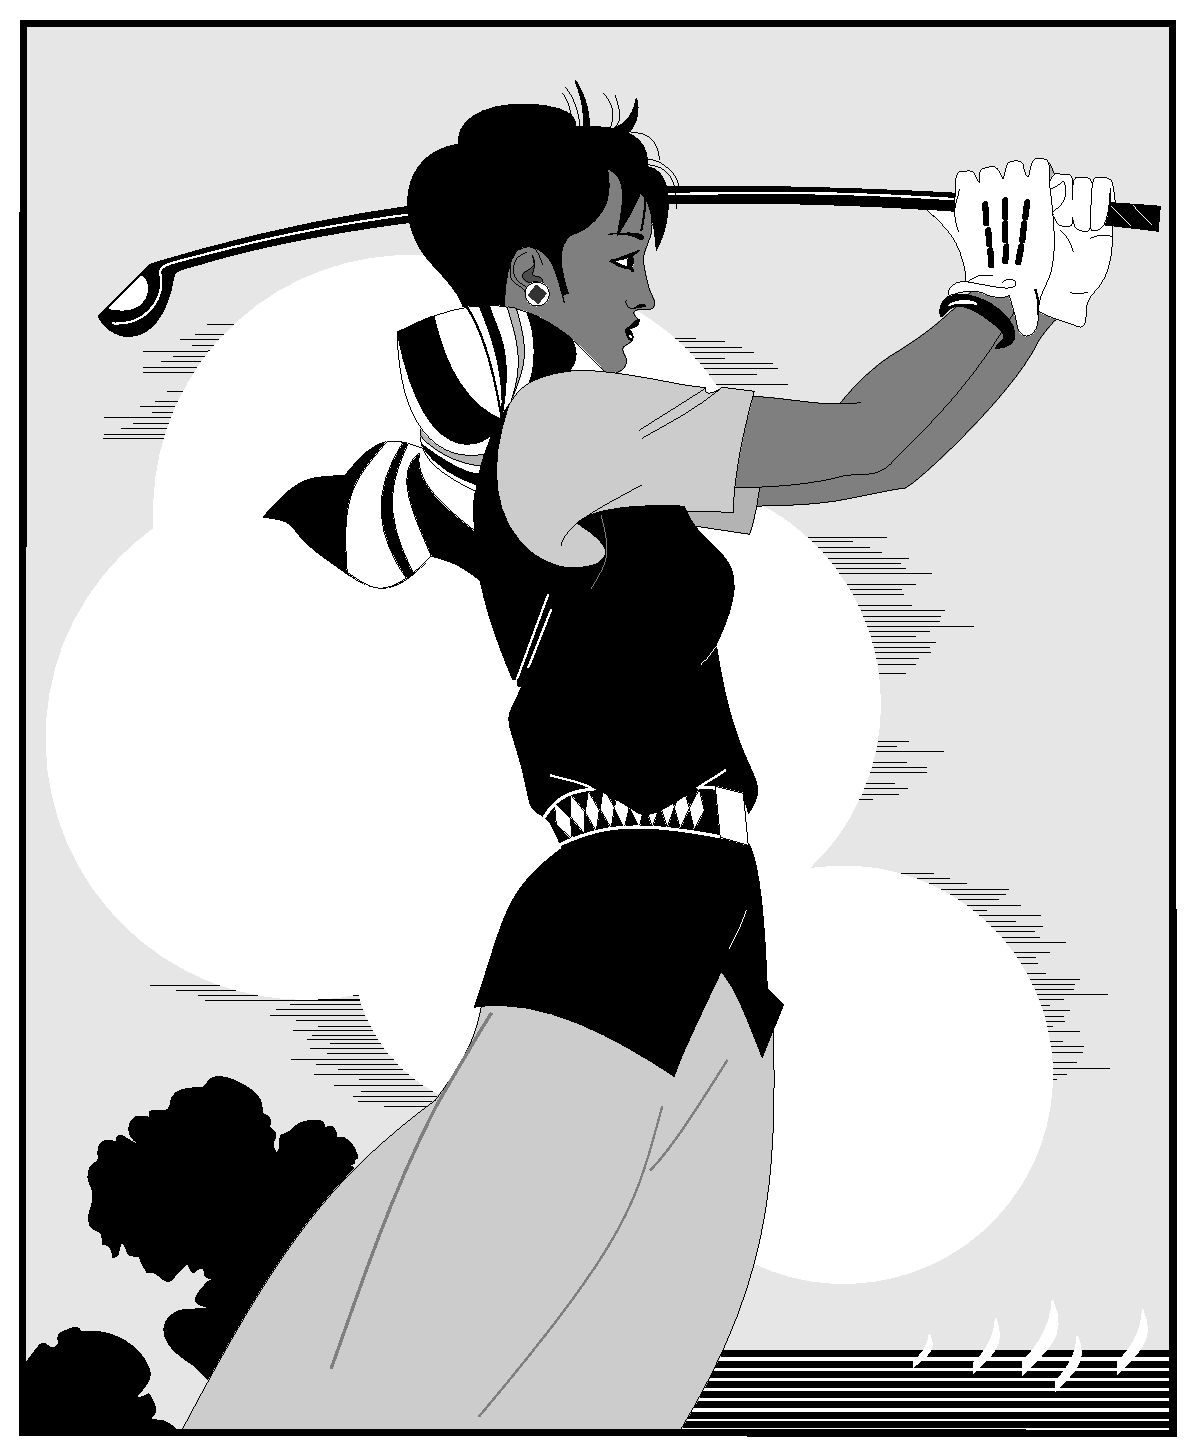
\includegraphics[width=0.2\textwidth]{golfer}}
			\fbox{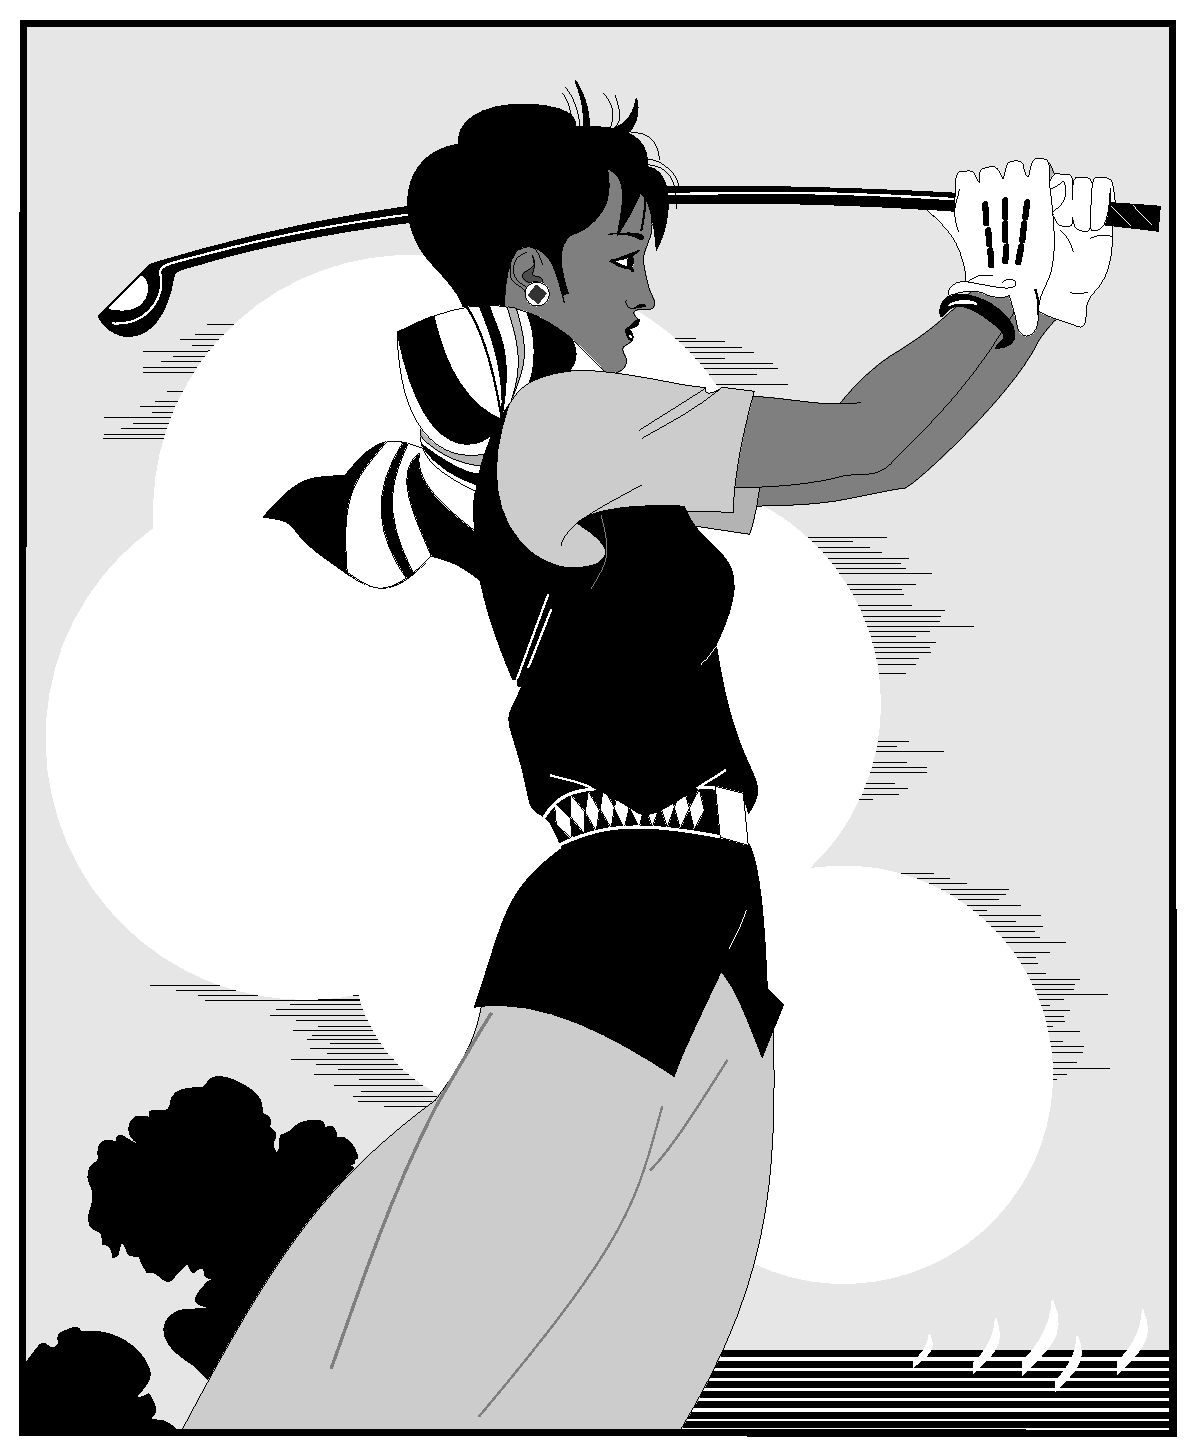
\includegraphics[width=0.2\textwidth]{golfer}}
			\fbox{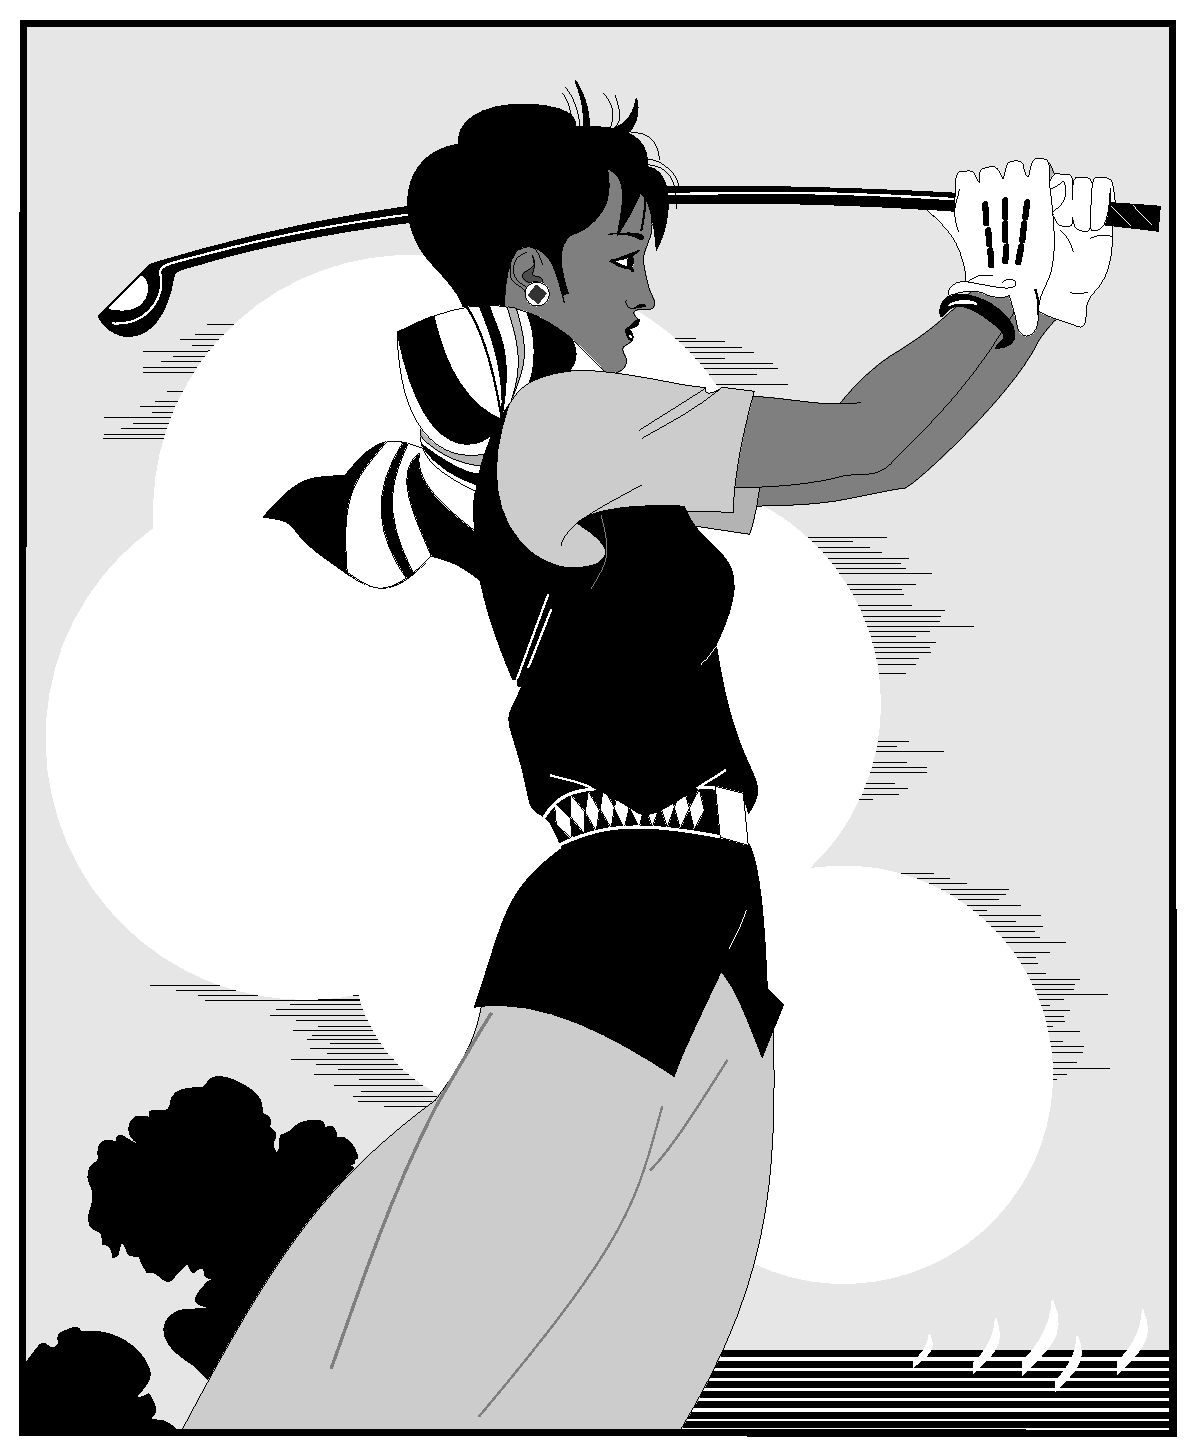
\includegraphics[width=0.2\textwidth]{golfer}}
			\fbox{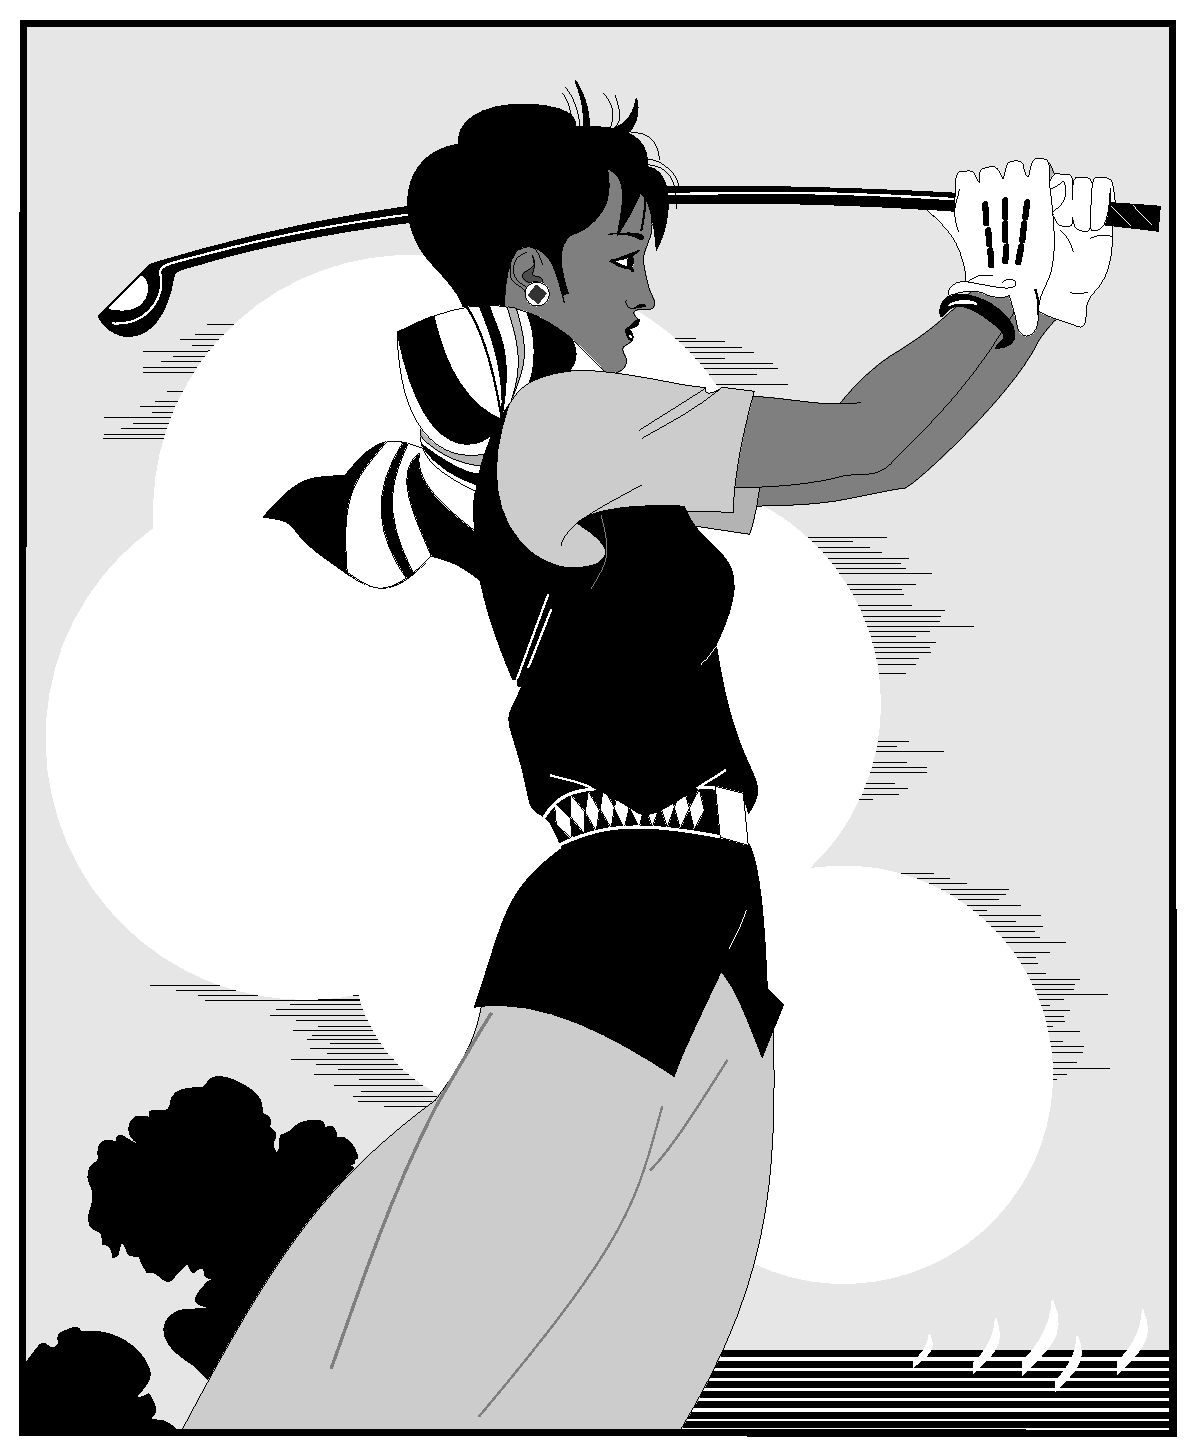
\includegraphics[width=0.2\textwidth]{golfer}}
\bicaption[golfer7]{}{打高尔夫球的人(非规范要求)}{Fig.$\!$}{The person playing golf (Not stated in the regulation)}
		\end{minipage}
	\end{sideways}
\end{figure}

\clearpage

如果不想让图片浮动到下一章节,那么在此处使用\cs{clearpage}命令。

\section{如何做出符合规范的漂亮的图}

关于作图工具在后文\ref{drawtool}中给出一些作图工具的介绍,此处不多言。
此处以R语言和Tikz为例说明如何做出符合规范的图。

\subsection{Tikz作图举例}

使用Tikz作图核心思想是把格式、主题、样式与内容分离,定义在全局中。
注意字体设置可以有两种选择,如何字少,用五号字,字多用小五。
使用Tikz作图不会出现字体问题,字体会自动与正文一致。

\begin{figure}[thb!]
  \centering
      \begin{tikzpicture}[xscale=0.8,yscale=0.3,rotate=90]
        \small
	\draw (-22,6.5) node[refcell]{参考基因组};
	\draw[refline] (-23, 5) -- (27, 5);
	\draw (-22,3.75) node[tscell]{肿瘤样本};
	\draw (-20,3.75) node[tncell]{正常细胞};
	\draw[tnline] (-21, 2.5) -- (27, 2.5);
	\draw (-20,1.25) node[ttcell]{肿瘤细胞};
	\rcell{2}{6};
	\draw[fakeevolve] (4.5, 5.25) -- (4.5, 4.8);
	\ncell{2}{4};
	\draw[evolve] (4.5, 3) .. controls (4.5,2.8) and (-3.5,2.9) ..  (-3.5, 2);
	\draw[evolve] (4.5, 3) .. controls (4.5,2.8) and (11.5,2.9) .. (11.5, 2);
	\tcellone{-6}{1.5};
	\draw (-9, 2) node[ttcell]{1};
	\draw[evolve] (-3.5, 0) .. controls (-3.5,-0.2) and (-12,-0.1) .. (-12, -1.5);
	\draw[evolve] (-3.5, 0) .. controls (-3.5,-0.2) and (1.5,-0.1) .. (1.5, -1.5);
	\tcellthree{7}{1.5};
	\draw (4, 2) node[ttcell]{2};
	\draw[evolve] (11, 0.5) .. controls (11,0.3) and (19,0.4) .. (19, -1.5);
	\tcellfive{-16}{-2};
	\draw (-19, -1.5) node[ttcell]{3};
	\tcelltwo{-1}{-2};
	\draw (-4, -1.5) node[ttcell]{4};
	\tcellfour{12}{-2};
	\draw (9, -1.5) node[ttcell]{5};
      \end{tikzpicture}
  \begin{minipage}{.9\linewidth}
      \vskip 0.2em
      \wuhao 图中,带有箭头的淡蓝色箭头表示肿瘤子种群的进化方向。一般地,从肿瘤组织中取用于进行二代测序的样本中含有一定程度的正常细胞污染,因此肿瘤的样本中含有正常细胞和肿瘤细胞。每一个子种群的基因组的模拟过程是把生殖细胞变异和体细胞变异加入到参考基因组中。
      \vspace{0.6em}
  \end{minipage}
\bicaption[tumor]{}{肿瘤组织中各个子种群的进化示意图}{Fig.$\!$}{The diagram of tumor subpopulation evolution process}
\end{figure}

\subsection{R作图}

R是一种极具有代表性的典型的作图工具,应用广泛。
与Tikz图~\ref{tumor}~不同,R作图分两种情况:(1)可以转换为Tikz码;(2)不可转换为Tikz码。
第一种情况图形简单,图形中不含有很多数据点,使用R语言中的Tikz包即可。
第二种情况是图形复杂,含有海量数据点,这时候不要转成Tikz矢量图,这会使得论文体积巨大。
推荐使用pdf或png非矢量图形。
使用非矢量图形时要注意选择好字号(五号或小五),和字体(宋体、新罗马)然后选择生成图形大小,注意此时在正文中使用\cs{includegraphics}命令导入时,不要像导入矢量图那样控制图形大小,使用图形的原本的
宽度和高度,这样就确保了非矢量图形中的文字与正文一致了。

为了控制\hitszthesis\ 的大小,此处不给出具体举例。

\subsection{专业绘图工具}[Processional drawing tool]
\label{drawtool}

推荐使用tikz包,使用tikz源码绘图的好处是,图片中的字体与正文中的字体一致。具体如
何使用tikz绘图不属于模板范畴。

tikz适合用来画不需要大量实验数据支撑示意图。但R语言等专业绘图工具具有画出各种、
专业、复杂的数据图。R语言中有tikz包,能自动生成tikz码,这样tikz几乎无所不能。
对于排版有极致追求的小伙伴,可以参考
\href{http://www.texample.net/tikz/resources/}{http://www.texample.net/tikz/resources/}
中所列工具,几乎所有作图软件所作的图形都可转成tikz,然后可以自由的在tikz中修改
图中内容,定义字体等等。实现前文窝工规范中要求的图中字体的一致性的终极目标。

\lipsum[1]

\section{本章小结}[Brief summary]

\lipsum[1]


% 第3章
% !TEX root = ../main.tex

% 中英标题:\chapter{中文标题}[英文标题]
\chapter{前端路径搜索算法及安全约束生成算法设计}\label{chap:front_end_algorithm}

\section{引言}\label{sec:intro_3}
基于优化的多旋翼无人机的轨迹规划过程一般可分为前端和后端两个部分:
\begin{enumerate}
  \renewcommand{\labelenumi}{(\theenumi)}
  \item 前端路径查找(front-end path search):利用地图信息在空间中搜寻出一条可行的无碰撞路径,路径由一系列路径点组成,是对飞行器运动的纯几何描述。
        因此路径查找工作在离散、低维的空间中。
        根据需要,前端算法还可以根据搜索出的路径得到四周安全无碰撞区域的几何描述(如前文提到的安全飞行走廊),作为后端优化的约束信息。
  \item 后端轨迹生成(back-end trajectory generation):在前端找到的可行路径和安全约束的基础上,根据动力学和运动学约束,通过拟合、优化的方法得到一条具备时间律的连续、平滑且安全的轨迹输入到飞行器的控制器中。
        因此轨迹生成工作在连续、高维的空间中。
\end{enumerate}

本章将为冗余驱动飞行器的轨迹规划器设计前端算法。
分别介绍$SE(3)$空间中RRT算法以及安全飞行走廊生成算法的设计与实现;

\section{路径搜索算法的设计}\label{sec:search_algorithm}
为实现OmniHex等冗余驱动多旋翼飞行器的路径搜索,有很多算法可供选择。
本节从算法选择、算法原理和算法实现三方面讲述路径搜索的算法设计。
\subsection{路径搜索算法概述}\label{subsec:path_search_overview}
目前常用的路径搜索算法种类非常多,大体上可以分为基于图搜索的和基于采样的两类。

在基于图搜索的算法中,比较有代表性的有Dijkstra算法、基于Dijkstra算法改进的A*算法\cite{hart1968formal}以及基于A*算法改进的跳点搜索(jump point search,JPS)\cite{harabor2011online},
这些算法同时具有完备性和最优性,即当可行解存在时就一定能找到可行解,并且这个可行解一定是所有可行解里最优的,
然而一个比较大的缺点是,这些算法需要按一定的分辨率将搜索空间离散化并存储每一个网格,
这就导致其内存占用量会随着搜索空间的维度增加呈指数上升,与此同时计算时间也会快速增加,
因此这类算法不适用于$SE(3)$空间等高维状态空间中的路径搜索。

与基于图搜索的算法有序地搜索离散化的构型空间不同,基于采样的路径搜索算法在连续的构型空间中进行随机采样以期找到可行解。
如概率路图(probalistic roadmap,PRM)算法\cite{kavraki1996probabilistic}使用随机采样得到的构型空间中的可行点构建无碰撞图,
并在图中使用图搜索得到图中从起点到终点最短路径;
快速探索随机树(rapidly-exploring random tree,RRT)\cite{lavalle1998rapidly}算法基于单次查询的信息、以起点为根节点增量式地构建树结构,
树触及终点后即可回溯出一条从起点到终点的可行路径。
PRM算法和RRT算法都是概率完备的\cite{kavraki1998analysis,frazzoli2002real},
即如果可行解存在,则它们搜索失败的概率会随着样本数趋向无穷大而衰减到0。
然而,PRM算法和RRT算法都不能保证解的最优性,
作为改进,2011年Karaman等人提出了这两种算法的渐进最优版本:PRM*和RRT*\cite{karaman2011sampling},
这两种算法可以保证可行解存在时能被找到,且随着样本数趋于无穷而收敛至全局最优。
在此基础上又发展出了加快RRT*收敛速率的Informed-RRT*\cite{gammell2014informed}、适用于高维空间的商空间RRT算法QRRT\cite{orthey2019rapidly}等。
基于采样的算法在内存消耗和计算时间方面相比基于搜索的算法更有优势。
\begin{figure}[!ht]
  \setlength{\subfigcapskip}{-1bp}
  \centering
  \begin{minipage}{\textwidth}
  \centering
  \subfigure{\label{fig:schem_diag_jps}}\addtocounter{subfigure}{-2}
  \subfigure{\subfigure[JPS示意图]{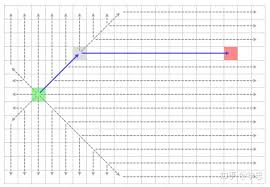
\includegraphics[width=0.3\textwidth]{jps.jpeg}}}
  \hspace{0.2em}
  \subfigure{\label{fig:schem_diag_prm}}\addtocounter{subfigure}{-2}
  \subfigure{\subfigure[PRM示意图]{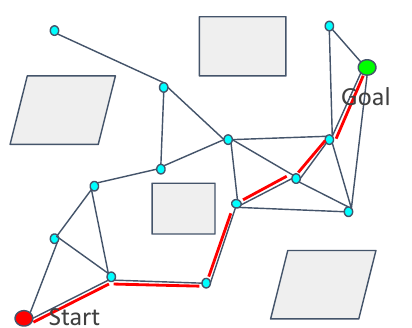
\includegraphics[width=0.3\textwidth]{prm.png}}}
  \hspace{0.2em}
  \subfigure{\label{fig:schem_diag_rrt}}\addtocounter{subfigure}{-2}
  \subfigure{\subfigure[RRT示意图]{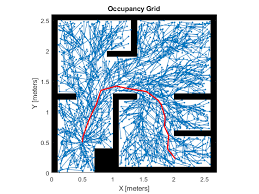
\includegraphics[width=0.3\textwidth]{rrt_2.png}}}
  \end{minipage}
  \caption{三种典型的路径搜索算法示意图\label{fig:three_methods_of_path_search}}
\end{figure}

本课题拟在$SE(3)$状态空间中为冗余驱动多旋翼飞行器搜索出一条可行路径,构型空间维度较高(6维)
且重点关注路径的安全性,并不优先考虑最优性,
故选择RRT算法作为前端路径搜索算法。
\subsection{$SE(3)$空间中的RRT算法}\label{subsec:rrt_in_SE3}
\subsubsection{RRT算法原理}\label{subsubsec:process_of_rrt}
如\ref{subsec:path_search_overview}节所述,RRT是一种通过随机构建空间填充树来高效搜索非凸高维空间的算法。
这棵树是以起始状态为根节点,根据从搜索空间中随机抽取的样本增量式构建的。
每次迭代都从搜索空间中采样出一个样本点,随后尝试从已有的树中距离样本点最近的节点向样本点以一定步长作延伸,到达一个新状态并形成一个运动基元,
如果该运动基元是有效的(比如全部位于无碰撞空间中,或满足某些其它的约束),则把这个运动基元和这个新状态分别作为边和节点加入树中,
这样整棵树就完成了一次生长。当新状态与目标状态的距离小于一定阈值且与目标状态的连接有效,则完成搜索。

本课题的$SE(3)$空间中的RRT算法完全遵循这些步骤,具体算法流程见算法\ref{alg:rrtse3}。

\begin{algorithm}[H]
  %\DontPrintSemicolon
  \wuhao
  \caption{$SE(3)$空间中的RRT算法\label{alg:rrtse3}}
  \begin{algorithmic}[1]
    \REQUIRE 地图$\mathcal{M}$、起始状态$\bm{x}_{init} \in SE(3)$、目标状态$\bm{x}_{goal} \in SE(3)$、\newline 
        最大迭代次数$n$、采样概率$p$和步长$\delta$ \\
    \ENSURE 从$\bm{x}_{init}$到$\bm{x}_{goal}$的一条可行路径$\varGamma$ \\
    \STATE 初始化搜索树$\mathcal{T}$,其中只有根节点$\bm{x}_{init}$ \\
    \FOR{$i = 1 \ to \ n$}
      \STATE 获得$\bm{x}_{sample}$:$\bm{x}_{sample}$有$p$的概率通过在搜索空间中均匀随机采样得到,有$(1-p)$的概率直接取$\bm{x}_{goal}$ \\
      \STATE 在搜索树$\mathcal{T}$中找到与$\bm{x}_{sample}$距离最近的节点$\bm{x}_{near}$ \\
      \STATE 从$\bm{x}_{near}$到$\bm{x}_{sample}$以步长$\delta$作插值,得到新状态$\bm{x}_{new}$ \\
      \IF {运动基元$(\bm{x}_{near} \rightarrow \bm{x}_{new})$无碰撞}
        \STATE 将$\bm{x}_{new}$作为新节点加入搜索树$\mathcal{T}$,并设置其父节点为$\bm{x}_{near}$\\
      \ENDIF
      \IF {$\bm{x}_{new}$与$\bm{x}_{goal}$之间的距离小于等于$\delta$且运动基元$(\bm{x}_{near} \rightarrow \bm{x}_{new})$无碰撞}
        \STATE 将$\bm{x}_{goal}$加入搜索树$\mathcal{T}$,并设置其父节点为$\bm{x}_{new}$ \\
        \STATE 从$\bm{x}_{goal}$根据父节点回溯出路径$\varGamma$ \\
        \STATE 结束循环 \\
      \ENDIF
    \ENDFOR
  \end{algorithmic}
\end{algorithm}

\subsubsection{$SE(3)$状态空间中的相关操作}\label{subsubsec:operations_in_SE3}
从算法\ref{alg:rrtse3}中可以看到,在搜索过程中需要对状态空间进行均匀采样,需要计算两个状态之间的距离,
在得到新状态以及对运动基元的有效性进行检测时还需要在两个状态之间进行插值。
即需要对$SE(3)$空间作采样、度量和插值三种操作。
$SE(3)$状态空间是一种复合的状态空间,由位置子空间$\mathbb{R}^3$和姿态子空间$SO(3)$构成,即$SE(3)=\mathbb{R}^3\times SO(3)$
在进行上述三种操作时可以先分别对两个子空间独立进行考虑,最后再进行整合。

位置子空间是欧几里得空间,在其中进行均匀采样就是分别对三个坐标值进行均匀采样;
两个位置之间的距离就是欧氏距离:
\begin{equation}
  \text{Dist}_{\mathbb{R}^3}(\bm{p}_1, \bm{p}_2) = \Vert \bm{p}_1 - \bm{p}_2 \Vert_2, \forall \bm{p}_1, \bm{p}_2 \in \mathbb{R}^3
  \label{equ:distance_in_R3}
\end{equation}
两个位置向量之间的线性插值如下式所示:
\begin{equation}
  \text{Interp}_{\mathbb{R}^3}(\bm{p}_1, \bm{p}_2; t) = 
  (1 - t)\bm{p}_1 + t\bm{p}_2, \forall \bm{p}_1, \bm{p}_2 \in \mathbb{R}^3, \forall t \in [0, 1]
  \label{equ:interpolation_in_R3}
\end{equation}

位置子空间中上述三种操作都很直接。
然而,在非欧的姿态子空间$SO(3)$中进行这些操作就显得不那么直观了。
一种比较朴素的做法是把$SO(3)$中的姿态用欧拉角表示,然后按$\mathbb{R}^3$空间中的方法来进行操作。
但是由于欧拉角的奇异性与周期性,使得欧氏空间中的度量方法并不能很好地反映姿态之间的差异。
比如,两组数值上差别很大的欧拉角可能表示的是两个相近甚至相同的姿态。
所以这种做法缺乏合理性。

\begin{figure}[ht]
  \centering
  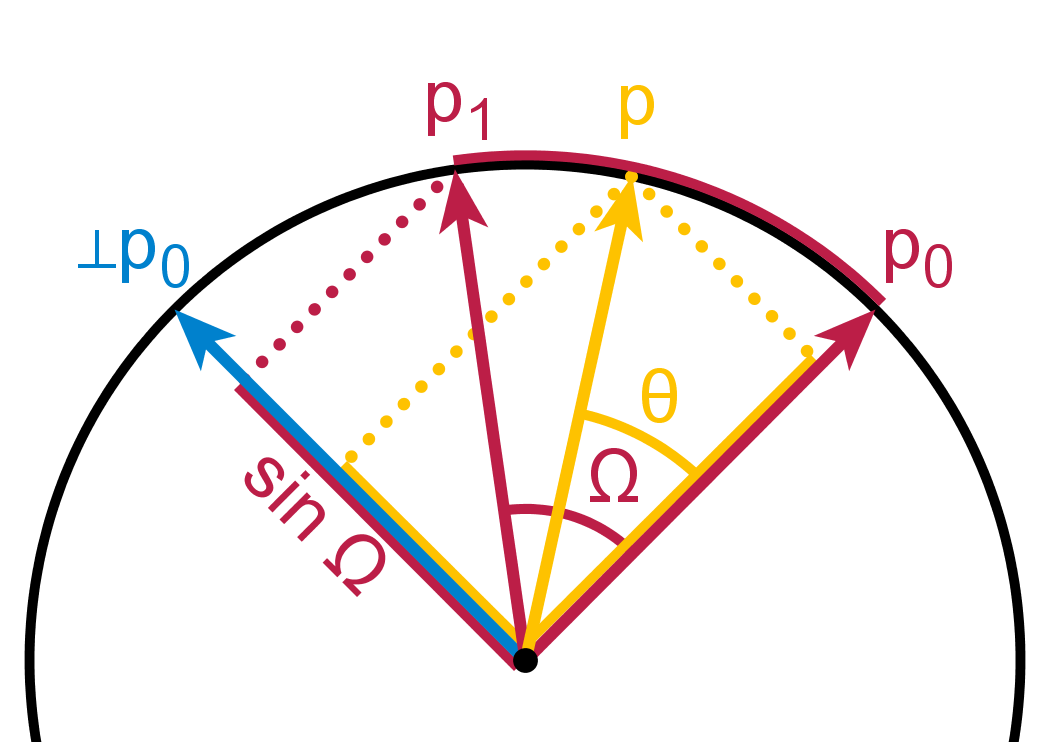
\includegraphics[width = 0.58\textwidth]{Slerp_factor_explanation.png}
  \caption{球面线性插值(slerp)示意图}
  \label{fig:slerp}
\end{figure}

本课题设计的RRT算法中对$SO(3)$空间的处理方式参考Kuffner等人于2004年提出的方法\cite{kuffner2004effective},
以上三种操作均基于四元数来进行,这样可以有效避免姿态表示的奇异性与重复性带来的缺点。
记表示绕轴$\bm{v} = \trans{[v_1 \quad v_2 \quad v_3]} \in \mathbb{R}^3$旋转角度$\theta \in \mathbb{R}$的单位四元数为:
\begin{equation}
  \bm{Q} = \trans{
    \begin{bmatrix}
      w & x & y & z
    \end{bmatrix}
  }
   = \trans{
     \begin{bmatrix}
       \cos{\frac{\theta}{2}} & v_1\cos{\frac{\theta}{2}} & v_2\cos{\frac{\theta}{2}} & v_3\cos{\frac{\theta}{2}}
     \end{bmatrix}
   }
   \label{equ:definition_of_unit_quaternion}
\end{equation}
则将在$SO(3)$空间中进行均匀采样可视为在单位四元数超球面上进行均匀采样,其流程如算法\ref{alg:uniform_unit_quaternion}所示;

\begin{algorithm}[H]
  \wuhao
  \caption{生成均匀分布的随机单位四元数\label{alg:uniform_unit_quaternion}}  
  \begin{algorithmic}[1] %每行显示行号  
      \REQUIRE 无  
      \ENSURE 均匀随机四元数$\bm{Q}=(w,x,y,z)$
      \STATE $s=uniform(0,1)$ // uniform(0,1)为生成0到1之间的均匀分布随机数
      \STATE $\sigma_{1}=\sqrt{1-s}$
      \STATE $\sigma_{2}=\sqrt{s}$
      \STATE $\theta_{1}=2\pi*uniform(0,1)$
      \STATE $\theta_{2}=2\pi*uniform(0,1)$
      \STATE $w=\cos(\theta_{2})*\sigma_{2}$
      \STATE $x=\sin(\theta_{1})*\sigma_{1}$
      \STATE $y=\cos(\theta_{1})*\sigma_{1}$
      \STATE $z=\sin(\theta_{2})*\sigma_{2}$
      \RETURN{$(w,x,y,z)$}
  \end{algorithmic}  
\end{algorithm} 

两个$SO(3)$状态间的距离定义为其在超球面上的弧长,即
\begin{equation}
  \text{Dist}_{SO(3)}(\bm{Q}_1, \bm{Q}_2) = \arccos(\trans{\bm{Q}_1}\bm{Q}_2), \forall \bm{Q}_1, \bm{Q}_2 \in SO(3)
  \label{equ:distance_in_SO3}
\end{equation}
在两个$SO(3)$状态间进行插值可视为在单位四元数超球面上进行球面线性插值(slerp,\figref{fig:slerp}),即:
\begin{equation}
  \text{Interp}_{SO(3)}(\bm{Q}_1, \bm{Q}_2; t) = 
  \frac{\sin[(1-t)\varOmega]}{\sin\varOmega}\bm{Q}_1 + \frac{\sin[t\varOmega]}{\sin\varOmega}\bm{Q}_2, 
  \forall \bm{Q}_1, \bm{Q}_2 \in SO(3), \forall t \in [0, 1]
  \label{equ:interpolation_in_SO3}
\end{equation}

现在已经分别确定了$SE(3)$中位置子空间和姿态子空间的采样、度量和插值的方法,
那么整个$SE(3)$空间中的采样和插值操作可以分别对其子空间进行,最后将得到的结果复合即可;
两个$SE(3)$状态的距离则可以表示如下:
\begin{equation}
  \text{Dist}_{SE(3)}(\bm{x}_1, \bm{x}_2) = 
  \sqrt{\text{Dist}_{\mathbb{R}^3}^2(\bm{p}_1, \bm{p}_2) + \text{Dist}_{SO(3)}^2(\bm{Q}_1, \bm{Q}_2)}, 
  \forall \bm{x}_1, \bm{x}_2 \in SE(3)
  \label{equ:distance_in_SE3}
\end{equation}
其中$\bm{p}_i \in \mathbb{R}^3$和$\bm{Q}_i \in SO(3)$分别为$\bm{x}_i \in SE(3)$的位置和姿态分量($i=1,2$)。
\subsection{近邻搜索}\label{subsuc:near_search}
RRT算法的另一个关键步骤是在已有的树中寻找出距离采样点$\bm{x}_{sample}$最近的节点,
这是一个近邻搜索问题,其耗时与待搜索集合中的元素个数$n$呈正相关,
也就是说,随着RRT算法迭代次数的增加,查找最近节点这一步的耗时也会随之增加,
所以这一步的效率是影响整个寻路算法效率的最重要因素之一。

近邻搜索最简单的方法就是线性搜索,其具有$O(n)$的时间复杂度。
显然,当$n$很大时线性搜索并不是一种高效的方法。
目前有许多用来存储带查找元素的数据结构可以加速搜索,
如Kd树\cite{bentley1975multidimensional}就是一种用来组织欧氏空间$\mathbb{R}^k$中点的数据结构,
在一棵平衡的Kd树中作最近邻搜索的平均时间复杂度为$O(\text{log}n)$;
1995年Brin提出的几何近邻搜索树(geometric near-neighbor access tree,GNAT)\cite{1995Near}只需要定义好距离函数就可以存储任意种类的数据点,
并且有相关实验能说明GNAT树在近邻搜索问题上的高效性。

根据本课题的需求,这里选择GNAT作为存储非欧空间$SE(3)$中点的数据结构。下面对GNAT的构建和基于GNAT的近邻搜索算法作简要介绍

\subsubsection{GNAT数据结构简介}\label{subsubsec:introduction_of_gnat}
GNAT是一种基于空间的分层超平面划分(hierarchical hyperplane partitioning)对度量空间(metric space)进行索引的数据结构。
在介绍GNAT的核心思想之前,先给出Dirichlet域的概念\cite{Engel1986}:
\begin{definition}[(Dirichlet域)]
  \label{def:dirichlet_domain}
  给定度量空间$M$,以及点集$P=\{\bm{x}_1,\cdots,\bm{x}_k\} \subset M$,
  点$\bm{x}_i \in P$的Dirichlet域$\mathbb{D}_{\bm{x}_i} \subset M$是$M$中所有满足下述条件的点$\bm{x}$的集合:
  \begin{equation}
    \text{Dist}(\bm{x}, \bm{x}_i) \leq \text{Dist}(\bm{x}_j,\bm{x}_i),\forall j \in \{1,\cdots,k\} \setminus \{i\}
    \label{condition_of_points_in_Dirichlet_domain}
  \end{equation}
\end{definition}

在GNAT树的根节点处,一系列分割点$X$被一种贪心策略从待存储的点集$S$中选出,
接着基于这些分割点将度量空间$M$划分为一系列Dirichlet域$\mathbb{D}_{\bm{x}_1},\cdots,\mathbb{D}_{\bm{x}_k}$,
剩下的点将根据它们落入的Dirichlet域分组,随后继续对这些分组重复上述步骤,最后递归地构建出GNAT。
\figref{fig:simple_gnat}展示了一棵简单的2层GNAT结构,
图中较大的点代表顶层节点(根节点)的分割点,较小的点代表子节点(叶节点)的分割点;
较粗的线代表顶层分割点对应区域的边界,而较细的线则代表底层分割点的。
\begin{figure}[ht]
  \centering
  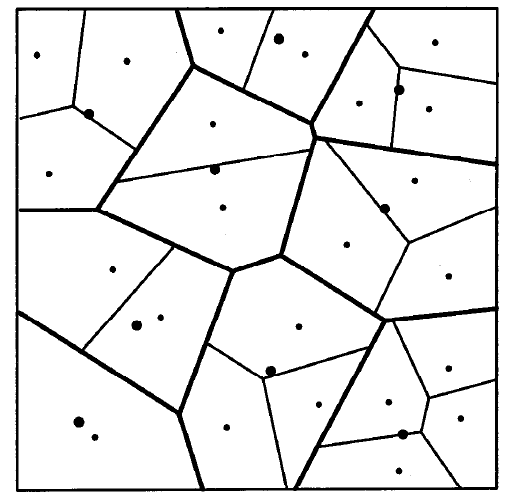
\includegraphics[width = 0.58\textwidth]{simple_gnat.png}
  \caption{一棵2层GNAT示意图}
  \label{fig:simple_gnat}
\end{figure}

GNAT树的基本构建过程叙述如下:
\begin{enumerate}
  \renewcommand{\labelenumi}{(\theenumi)}
  \item 从待组织的数据集中用贪心策略选出相隔足够远的$k$个分割点$\bm{x}_1,\cdots,\bm{x}_k$;
  \item 将数据集中剩下的点与最近的分割点相关联,并将与分割点$\bm{x}_i$相关联的点的集合记为$D_{\bm{x}_i}$;
  \item 对每对分割点$(\bm{x},\bm{x}_j)$,计算如下距离范围:
  \begin{equation}
    \text{range}(\bm{x_i}, D_{\bm{x}_j}) = [\text{minDist}_M(\bm{x_i}, D_{\bm{x}_j}), \text{maxDist}_M(\bm{x_i}, D_{\bm{x}_j})]
  \end{equation},用于搜索时的剪枝操作;
  \item 递归地对每个$D_{\bm{x}_i}$重复上述过程。
\end{enumerate}

\subsubsection{基于GNAT的近邻搜索}\label{subsubsec:near_search_based_on_gnat}
给定一个点$\bm{x}$,若要在GNAT中搜索出所有与$\bm{x}$的距离在$r$之内的所有点($r$-近邻点),
除了充分利用GNAT所表达的数据集的固有几何信息外,还可以利用距离信息进行剪枝以提高效率。
如\figref{fig:gnat_branch_prunning}所示,因为$\text{Dist}(\bm{x}, \bm{p}) + r < \text{min\_d}(\bm{p}, D_{\bm{p}_i})$,
所以$D_{\bm{p}_i}$中就一定不存在$\bm{x}$的$r$-近邻点,这样$D_{\bm{p}_i}$对应的子节点就可以被剪除。
\begin{figure}[ht]
  \centering
  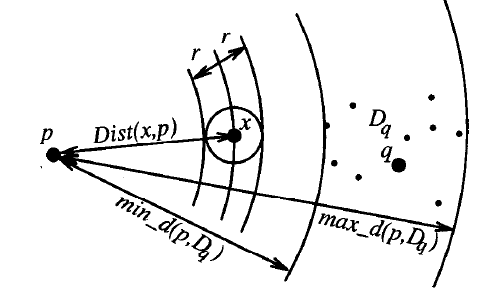
\includegraphics[width = 0.58\textwidth]{gnat_branch_prunning.png}
  \caption{利用距离信息在$r$-近邻搜索中进行剪枝的原理图}
  \label{fig:gnat_branch_prunning}
\end{figure}

在GNAT中进行$r$-近邻搜索的步骤叙述如下:
\begin{enumerate}
  \renewcommand{\labelenumi}{(\theenumi)}
  \item 记$P$为当前可能包含$\bm{x}$的$r$-近邻点的节点(初始状态下为根节点)的分割点,初始时$P$包含当前节点所有的分割点;
  \item 不重复地取一点$\bm{y} \in P$,若$\text{Dist}_M(\bm{x}, \bm{y}) \leq r$,则将$\bm{y}$加入结果中 \label{itm:pick_a_point_from_P};
  \item 考察所有$\bm{x}_i \in P$,如果有$[\text{Dist}_M(\bm{x}, \bm{y}_i)-r, \text{Dist}_M(\bm{x}, \bm{y}_i)+r] \cap \text{range}(\bm{y}, D_{\bm{x}_i}) = \emptyset$,则将$\bm{x}_i$从$P$中移除 \label{itm:prunning};
  \item 重复步骤\ref{itm:pick_a_point_from_P}和\ref{itm:prunning},直到$P$中所有点都试过一遍;
  \item 对$P$中剩下的所有点$\bm{y}_i$,递归地对$D_{\bm{y}_i}$进行搜索。
\end{enumerate}

如果要得到数据集中距离给定的$\bm{x}$最近的点,可以先基于Dirichlet域找到$\bm{x}$在GNAT中所在的叶节点,
随后在叶节点中线性搜索出其中距离$\bm{x}$最近的点,记这个最小距离为$r'$;
接着搜索出$\bm{x}$的所有$r'$-近邻点,
最后再对这些$r'$-近邻点进行线性搜索得到精确$\bm{x}$的最近邻。

为说明GNAT在近邻搜索上的高效性,本课题随机生成了$10^5$个Eigen三维双精度浮点型向量,分别基于线性搜索和GNAT做最近邻搜索。
经过数次集重复试验,每次都生成不同的随机点集,发现二者耗时均很稳定,
线性搜索平均耗时为34.6毫秒,而GNAT平均耗时仅为0.105毫秒,
二者相差数百倍,根据这个结果可以认为基于GNAT的近邻搜索之于线性搜索有巨大的优势。

以上介绍了基于GNAT的近邻搜索的通用方法,在本课题的应用场景中,
对应的度量空间$M$就是$SE(3)$空间,而GNAT所存储的就是当前的搜索树的所有节点。

\subsection{有效性检测}\label{subsec:validaty_checking}
在RRT算法中涉及两种有效性检测,一种是判断搜索空间中的单个状态是否有效,
另一种是基于单个状态的有效性检测来判断一个运动基元是否有效。

在本课题所设计的$SE(3)$空间的RRT算法(算法\ref{alg:rrtse3})中,
对状态和运动有效性的判断标准是其是否让飞行器与障碍物发生碰撞。
因为需要同时考虑飞行器的位置和姿态,且考虑到在狭小空间内实现轨迹规划的最终目标,
有必要在前端路径搜索时就考虑飞行器的形状。

\begin{figure}[ht]
  \centering
  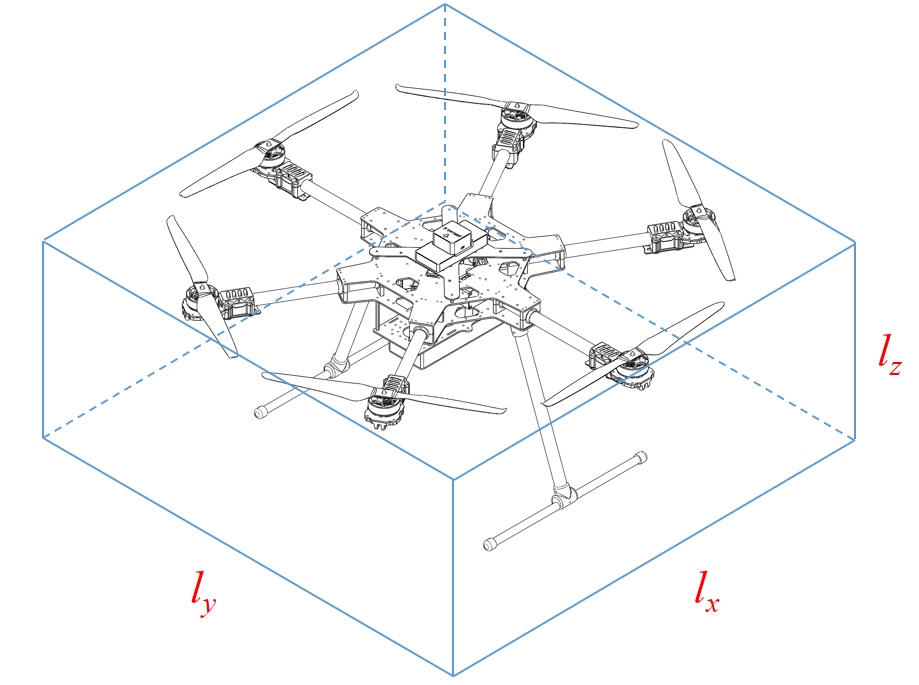
\includegraphics[width = 0.62\textwidth]{approximate_cuboid.png}
  \caption{将飞行器的形状近似为长方体}
  \label{fig:approximate_cuboid}
\end{figure}

如\figref{fig:approximate_cuboid}所示,这里将飞行器的形状简化为一个以其质心为中心、棱始终与机体坐标系保持一致的长方体。
则判断单个$SE(3)$状态是否有效,就转化为判断代表飞行器的长方体在这个状态对应的位置和姿态下是否与障碍物无交集,
而判断运动基元是否有效则可以在其上离散地取点(需要用到插值),若每个点对应的状态都是有效的,则认为该运动基元有效。
因此,本小节着重考虑单个状态的有效性检测。

在本课题所编写的RRT算法框架中,借鉴开源运动规划库OMPL\cite{sucan2012open}的思想,
将有效性检测这一操作抽象为StateValidityChecker和MotionValidityChecker两个抽象基类,
其中有纯虚函数isValid()作为提供给RRT算法主体的有效性检测公共接口,
如果要采用不同的有效性检测方法,只需继承StateValidityChecker或MotionValidityChecker抽象基类,实现其isValid()接口即可,
这样就实现了RRT算法主体与有效性检测的分离,提高了算法的复用性。

本课题根据地图形式的不同实现了基于点云的状态有效性检测和基于八叉树的状态有效性检测两种方法,
下面分别作简要说明。

\subsubsection{基于点云的状态有效性检测}\label{subsubsec:vc_based_on_pcl}
基于障碍物点云地图进行状态有效性检测的思路比较简单,
只要检查点云中是否有障碍物点落在给定$SE(3)$状态下的长方体内即可,有则无效,无则有效。
但如果单纯地使用线性搜索就必须要遍历整个点云,这对于稠密的点云来说非常的低效。
\begin{figure}[ht]
  \centering
  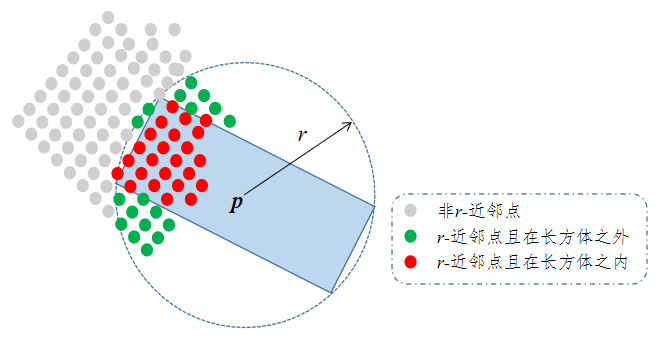
\includegraphics[width = 0.62\textwidth]{point_cloud_validity_checking.png}
  \caption{使用近邻搜索对有效性检测进行优化}
  \label{fig:point_cloud_validaty_checking}
\end{figure}

为解决这个问题,考虑使用GNAT数据结构来存储点云,配合近邻搜索来加速有效性检测过程。
如\figref{fig:point_cloud_validaty_checking}所示,长方体中心的位置为$\bm{p} \in \mathbb{R}^3$,
对$\bm{p}$进行近邻搜索得到其在点云中所有的$r$-近邻点,其中$r=\sqrt{l_x^2+l_y^2+l_z^2}/2$为长方体的外接球半径,
然后遍历所有$r$-近邻点检查是否有点位于长方体内,具体流程见算法\ref{alg:validaty_checking_based_on_point_cloud}。
\begin{algorithm}
  \wuhao
  \caption{基于障碍物点云的状态有效性检测\label{alg:validaty_checking_based_on_point_cloud}}  
  \begin{algorithmic}[1] %每行显示行号  
      \REQUIRE 用GNAT组织好的障碍物点云$\mathcal{P}$,待检测状态$\bm{x} \in SE(3)$, \newline
               长方体尺寸$(l_x, l_y, l_z)$,
               地图下界$\bm{b}_l \in \mathbb{R}^3$和上界$\bm{b}_u \in \mathbb{R}^3$
      \ENSURE 状态$\bm{x}$是否有效
      \STATE 计算长方体外接球半径$r=\sqrt{l_x^2+l_y^2+l_z^2}/2$
      \STATE 根据尺寸$(l_x, l_y, l_z)$和状态$\bm{x}$求出长方体各顶点的坐标$\bm{V}=[\bm{v}_1 \ \cdots \ \bm{v}_8]$
      \FOR {$i = 1 \ to \ 8$}
        \IF{$\bm{v}_i$超出地图上下界}
          \RETURN{False}
        \ENDIF
      \ENDFOR
      \STATE 在$\mathcal{P}$中搜索出长方体中心点$\bm{p}$($\bm{x}$的位置分量)的$r$-近邻点,构成点集$\mathcal{N}$
      \FORALL {$\bm{p}_{near} \in \mathcal{N}$}
        \IF{$\bm{p}_{near}$落在了长方体内}
          \RETURN{False}
        \ENDIF
      \ENDFOR
      \RETURN{True}
  \end{algorithmic}  
\end{algorithm} 

下面分析这种方法对有效性检测效率的改进程度。
令一次线性搜索有效性检测耗时为$T_1$,经由近邻搜索改进后的一次有效性检测耗时为$T_2$,
其中线性遍历检测整个点云耗时$T_{\text{linear}}$,使用GNAT获取$r$-近邻点耗时$T_{\text{GNAT}}$,线性遍历检测所有$r$-近邻点耗时$T_{r}$,
则有:
\begin{align}
  T_1 &\approx T_{\text{linear}} \label{equ:time_for_linear_validity_checking} \\
  T_2 &\approx T_{\text{GNAT}} + T_r \label{equ:time_for_optimized_validity_checking}
\end{align}
再令$T_{\text{GNAT}} = \lambda_1T_{\text{linear}}$,$T_r = \lambda_2T_{\text{linear}}$,
那么通常有$\lambda_1 \ll 1$,比如在\ref{subsubsec:near_search_based_on_gnat}节给出的例子中,就有$\lambda_1 < 1/300$;
$\lambda_2$近似为$r$-近邻点数量与点云中点的总数量的比值,通常也有$\lambda_2 \ll 1$,
故大多数情况下,$\lambda_1 + \lambda_2 \ll 1$,于是就有
\begin{equation}
  T_2 \approx (\lambda_1 + \lambda_2)T_1 \ll T_1
\end{equation}
这说明使用GNAT近邻搜索使有效性检测效率相比于暴力线性搜索有相当大的改进,
实际对比测试也支持这一结论。

\subsubsection{基于八叉树地图的状态有效性检测}\label{subsubsec:vc_based_on_pcl}
本课题中基于八叉树地图的状态有效性检测是通过调用FCL(flexible collision library)\cite{pan2012fcl}实现的。
FCL库提供了与八叉树地图库OctoMap\cite{hornung2013octomap}的接口,
可以很方便地检测不同几何形状(如代表飞行器的长方体)在不同位姿下与障碍物的碰撞。

\subsection{算法效果}\label{subsec:performance_of_rrtse3}
本小节展示所设计的$SE(3)$空间中的RRT算法使用基于点云和基于八叉树地图两种有效性检测方法的搜索效果,
并且每种方法都分别在障碍物稀疏及穿越狭窄通道两种场景下进行测试。测试中设置步长为0.8,采样概率为0.9。
\begin{figure}[!ht]
  \setlength{\subfigcapskip}{-1bp}
  \centering
  \begin{minipage}{\textwidth}

  \centering
  \subfigure{\label{fig:rrtse3_octomap_in_sparse_env_overview}}\addtocounter{subfigure}{-2}
  \subfigure{\subfigure[障碍稀疏(整体)]{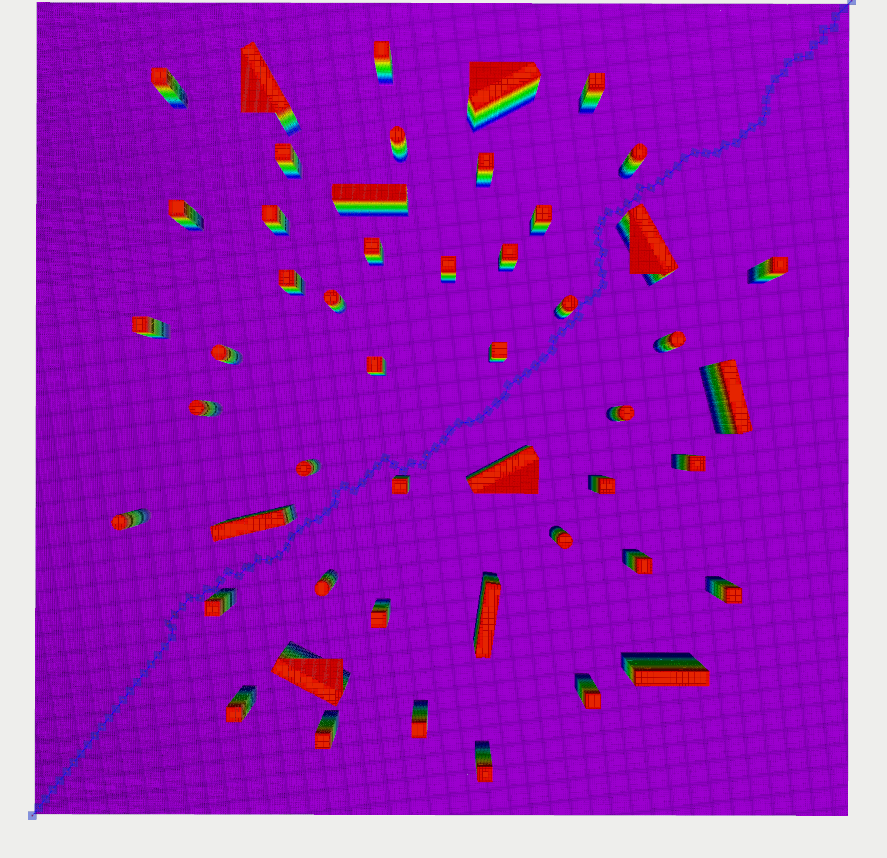
\includegraphics[width=0.23\textwidth]{octomap_rrtse3_1_overview.png}}}
  \hspace{0.2em}
  \subfigure{\label{fig:rrtse3_octomap_in_sparse_env_detail}}\addtocounter{subfigure}{-2}
  \subfigure{\subfigure[障碍稀疏(局部)]{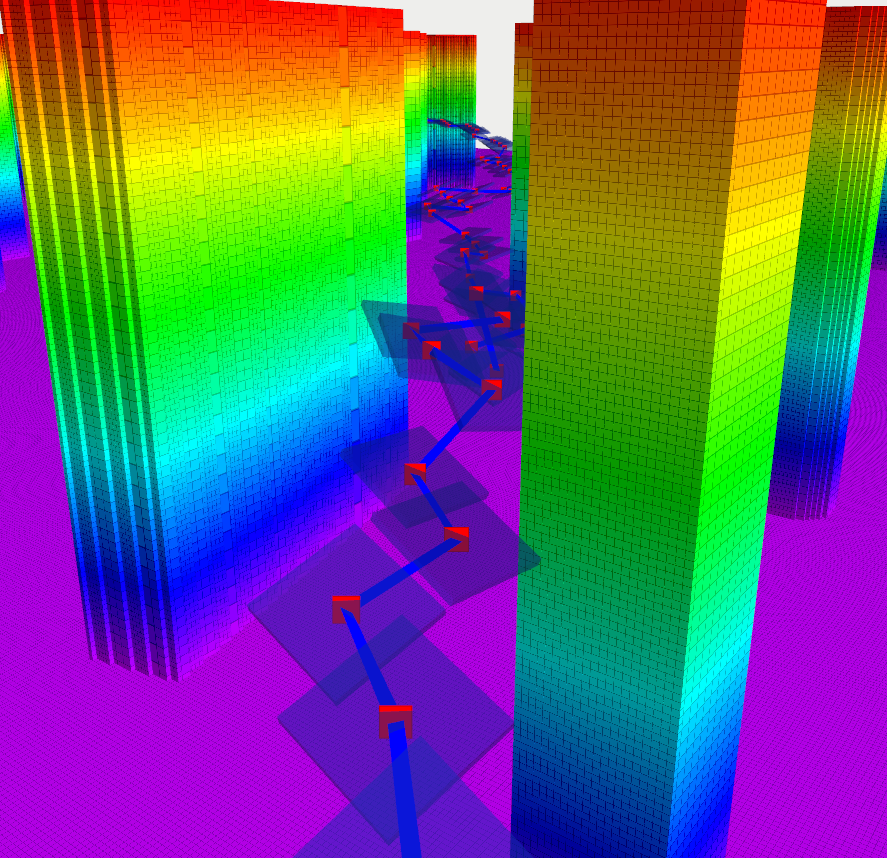
\includegraphics[width=0.23\textwidth]{octomap_rrtse3_1_detail.png}}}
  \hspace{0.2em}
  \subfigure{\label{fig:rrtse3_octomap_in_narrow_passage_overview}}\addtocounter{subfigure}{-2}
  \subfigure{\subfigure[狭窄通道(整体)]{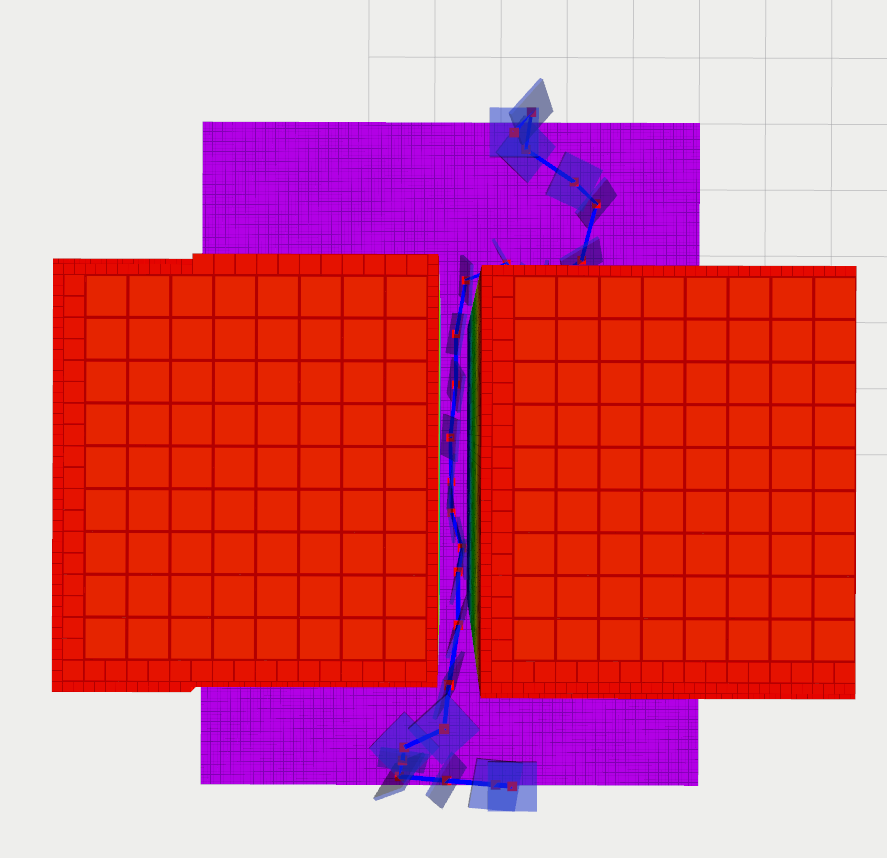
\includegraphics[width=0.23\textwidth]{octomap_rrtse3_2_overview.png}}}
  \hspace{0.2em}
  \subfigure{\label{fig:rrtse3_octomap_in_narrow_passage_detail}}\addtocounter{subfigure}{-2}
  \subfigure{\subfigure[狭窄通道(局部)]{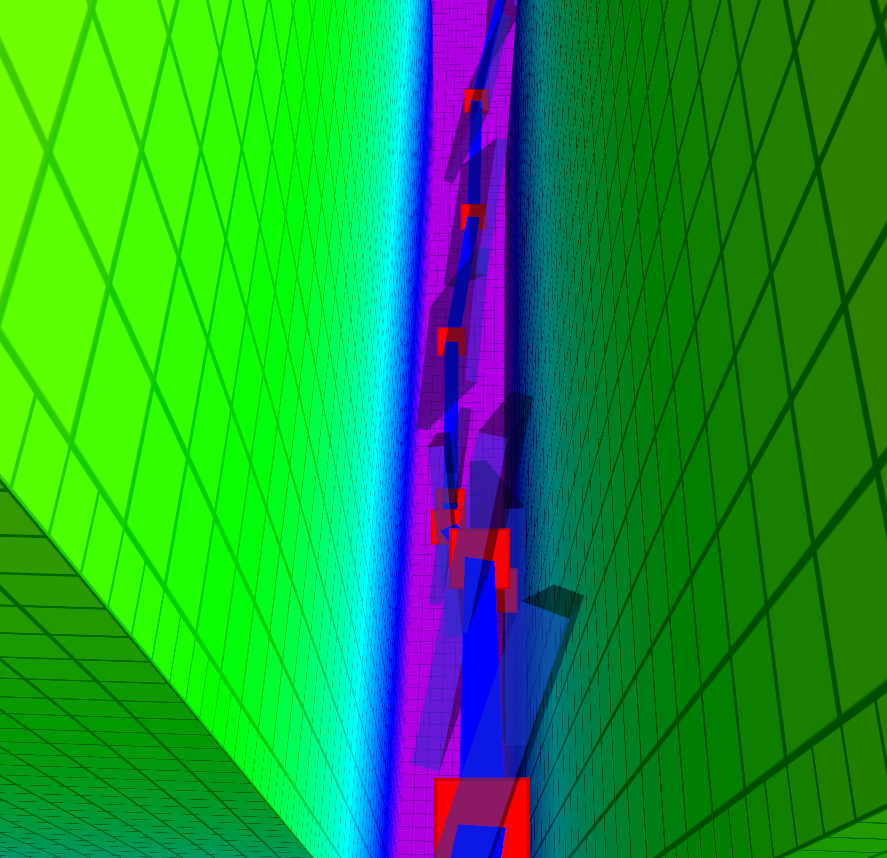
\includegraphics[width=0.23\textwidth]{octomap_rrtse3_2_detail.png}}}
  
  \end{minipage}
  \caption{$SE(3)$空间RRT算法效果可视化结果(基于八叉树地图)}
  \label{fig:performance_of_rrtse3_octomap}
\end{figure}

如\figref{fig:performance_of_rrtse3_octomap}所示为使用基于八叉树地图的有效性检测方法时的可视化结果。
图中蓝色半透明的长方体可视化表达了路径上每个$SE(3)$状态,
可见算法无论在宽松的环境中还是狭窄的环境中均能成功搜索出一条无碰撞路径,说明有效性检测成功发挥了其作用,
\figref{fig:rrtse3_octomap_in_narrow_passage_overview}中路径起点和终点附近的弯曲也表现出了RRT算法无法保证解的最优性的性质,
后续应用时将通过一定策略对路径点数量进行缩减来改善RRT的解中可能存在的这种局部的“舍近求远”现象。

\begin{figure}[!ht]
  \setlength{\subfigcapskip}{-1bp}
  \centering
  \begin{minipage}{\textwidth}

  \centering
  \subfigure{\label{fig:rrtse3_pcl_in_sparse_env_overview}}\addtocounter{subfigure}{-2}
  \subfigure{\subfigure[障碍稀疏(整体)]{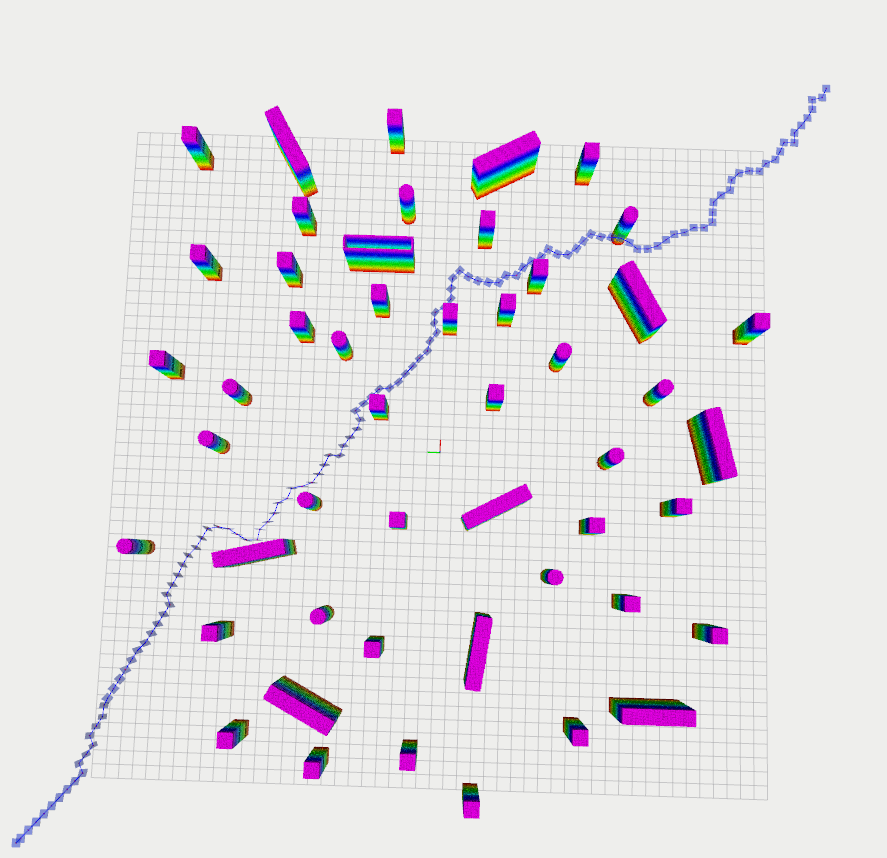
\includegraphics[width=0.23\textwidth]{point_cloud_rrtse3_1_overview.png}}}
  \hspace{0.2em}
  \subfigure{\label{fig:rrtse3_pcl_in_sparse_env_detail}}\addtocounter{subfigure}{-2}
  \subfigure{\subfigure[障碍稀疏(局部)]{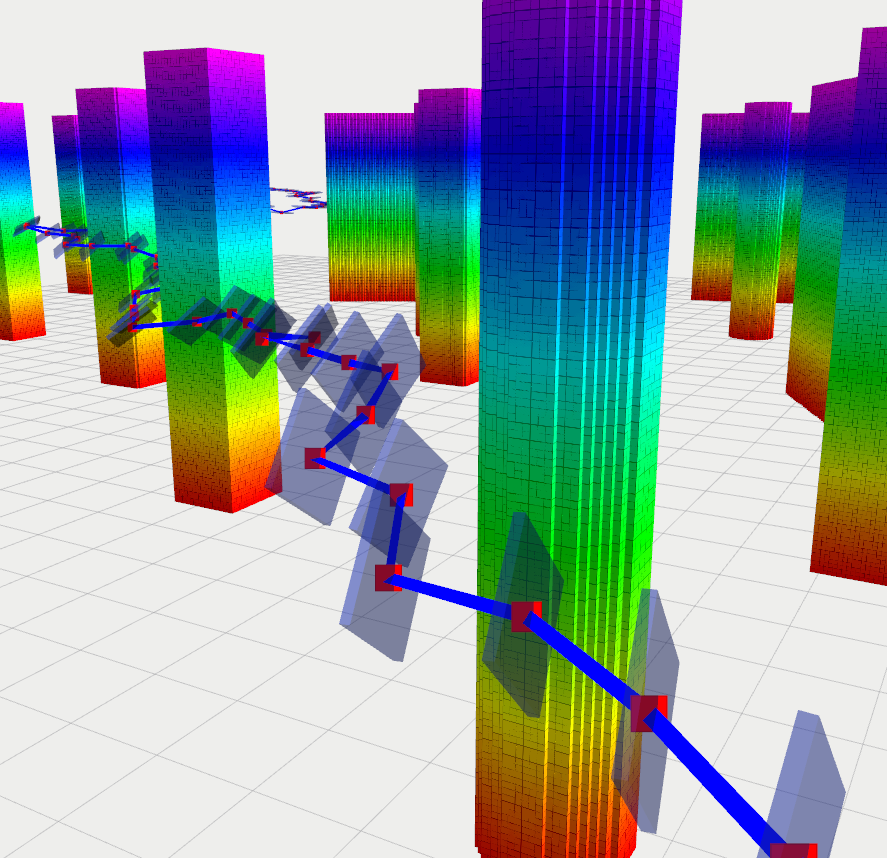
\includegraphics[width=0.23\textwidth]{point_cloud_rrtse3_1_detail.png}}}
  \hspace{0.2em}
  \subfigure{\label{fig:rrtse3_pcl_in_narrow_passage_overview}}\addtocounter{subfigure}{-2}
  \subfigure{\subfigure[狭窄通道(整体)]{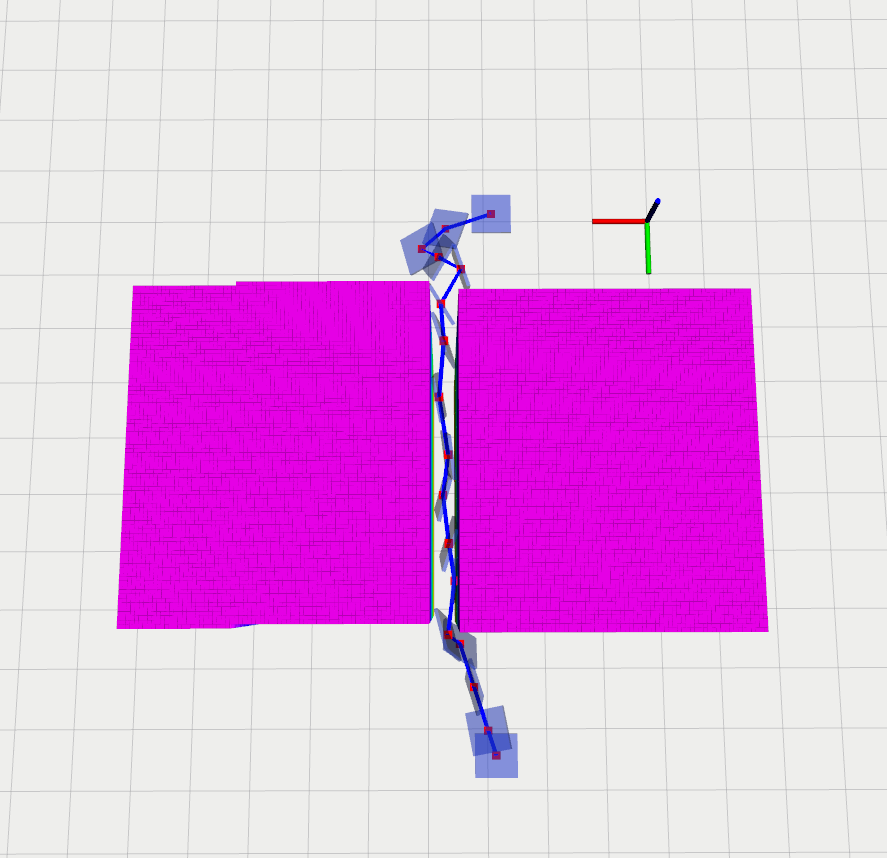
\includegraphics[width=0.23\textwidth]{point_cloud_rrtse3_2_overview.png}}}
  \hspace{0.2em}
  \subfigure{\label{fig:rrtse3_pcl_in_narrow_passage_detail}}\addtocounter{subfigure}{-2}
  \subfigure{\subfigure[狭窄通道(局部)]{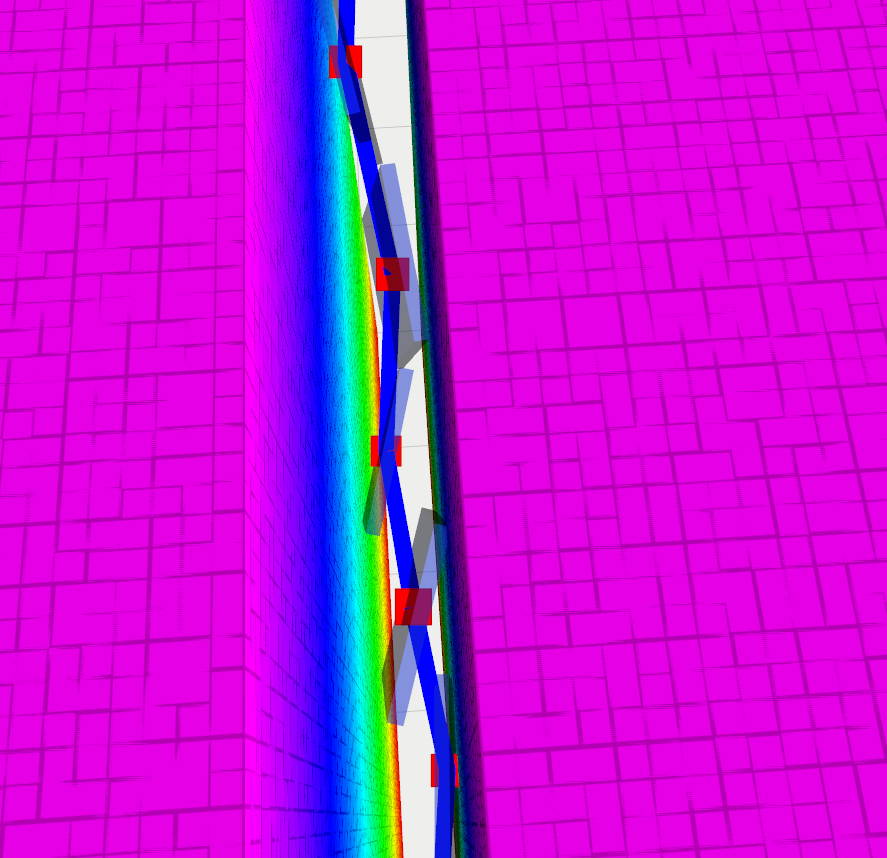
\includegraphics[width=0.23\textwidth]{point_cloud_rrtse3_2_detail.png}}}
  
  \end{minipage}
  \caption{$SE(3)$空间RRT算法效果可视化结果(基于点云地图)}
  \label{fig:performance_of_rrtse3_pcl}
\end{figure}

如\figref{fig:performance_of_rrtse3_pcl}所示为使用基于点云的有效性检测方法时的可视化结果,
可见得到的解与基于八叉树的方法并无很大区别。

\tabref{tab:rrtse3_performance_data}中列出了测试中所得到的一些数据。
可以看出狭窄环境的迭代次数要多于宽松的环境,
这是因为狭窄环境中可行区域占比更小,在一定迭代次数内找到解的概率就会更低。
而且可以注意到,同样环境和起终点条件下,
使用点云方法的求解时间显著高于使用八叉树方法,
这是由于这里的点云地图中障碍物内部也被填充,导致点的数量异常庞大,极大地增加了有效性检测的负担;
而基于八叉树的方法检测只需要用到障碍物表面信息。
如果在生成点云时能够合理地控制点的数量,尽量剔除冗余点,就能使点云法的求解速度大大提高;
在后文中所用到的一个50m$\times$50m大小、障碍物较为稠密的随机地图中,使用点云法可以在数百毫秒内搜索出一条对角路径。
另外,利用OctoMap库和PCL库\cite{rusu20113d}可以很方便地在点云和八叉树之间进行转换,
可以根据实际需求灵活地选择地图形式。

\begin{table}[htbp]
  \caption{关于$SE(3)$空间RRT算法的一些数据\label{tab:rrtse3_performance_data}}
  \vspace{0.5em}\centering\wuhao
  \begin{tabular}{ccccccc}
  \toprule[1.5pt]
  环境 & 地图类型 & 地图尺寸(m) & 起点(m) & 终点(m) & 迭代次数数量级 & 平均耗时\\
  \midrule[0.2pt]
  宽松 & 八叉树 & $60\times60\times6$ & $(29, -29, 3)$ & $(-29, 29, 3)$ & $10^2$ & 20毫秒左右\\
  宽松 & 点云 & $60\times60\times6$ & $(29, -29, 3)$ & $(-29, 29, 3)$ & $10^2$ & 数秒\\
  狭窄 & 八叉树 & $7.5\times10\times6$  & $(3, 1, 3)$ & $(3, 9, 3)$ & $10^3$ & 200毫秒以内\\
  狭窄 & 点云 & $7.5\times10\times6$  & $(3, 1, 3)$ & $(3, 9, 3)$ & $10^3$ & 数十秒\\
  \bottomrule[1.5pt]
  \end{tabular}
\end{table}

\section{3D安全飞行走廊生成算法的设计}\label{sec:sfc_gen_algorithm}
3D空间中的安全飞行走廊(SFC)一般用来描述无障碍物的空闲空间(free space),
一般用一系列球或凸多面体来表示,在无人机的轨迹规划中取得了许多应用\cite{han2021fast,mohta2018fast,gao2019flying}。
SFC通常在轨迹规划框架的前端部分根据初始路径生成,然后作为轨迹优化的约束给到后端。
目前SFC的生成方法也有多种,如Liu等人的RILS算法\cite{2017Planning}、Deits等人的IRIS方法\cite{deits2015computing}等。
本课题使用前者,下面对其进行简要介绍。
\subsection{算法原理}\label{subsec:design_of_sfc_gen_algorithm}
记障碍物点云为$\mathcal{O}$,本算法对$\mathbb{R}^3$空间进行操作,只需要$SE(3)$路径的位置部分,
记无碰撞位置路径为$P = \langle \bm{p}_0 \rightarrow \cdots \rightarrow \bm{p}_s \rangle$,
则算法将在每条线段$L_i = \langle \bm{p}_i \rightarrow \bm{p}_{i+1} \rangle$周围生成一个包含无碰撞空间的凸多面体$P_i$,
此过程分为两步,简述如下:
\subsubsection{无碰撞椭球的生成}
\begin{figure}[ht]
  \centering
  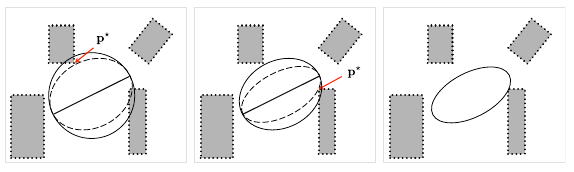
\includegraphics[width = 0.83\textwidth]{get_ellipsoid.png}
  \caption{生成无碰撞椭球示意图}
  \label{fig:get_ellipsoid}
\end{figure}
一个椭球$\xi$可以表示为如下形式:
\begin{equation}
  \xi(\bm{E}, \bm{d}) = \{\bm{p} = \bm{E}\bar{\bm{p}} + \bm{d} \mid \Vert \bar{\bm{p}} \Vert \leq 1 \}
  \label{equ:representation_of_ellipsoids}
\end{equation}

对于一个$\mathbb{R}^3$中的椭球来说,变换矩阵$\bm{E}$可以分解为旋转变换加缩放变换,即:
\begin{equation}
  \bm{E} = \trans{\bm{R}}\bm{S}\bm{R} = \trans{\bm{R}}\text{diag}(a, b, c)\bm{R}
  \label{equ:decomp_E}
\end{equation}
其中$a, b, c$分别为椭球坐标系的$\tilde{x}, \tilde{y}, \tilde{z}$轴对应的缩放系数。
任意一点到椭球的距离定义如\equref{equ:distance_to_ellipsoids},若$\rho(\bm{p}, \xi) < 1$,则$\bm{p}$位于椭球内部。
\begin{equation}
  \rho(\bm{p}, \xi(\bm{E}, \bm{d})) = \Vert \bar{\bm{p}} \Vert = 
  \Vert \bm{E}^{-1}(\bm{p} - \bm{d}) \Vert
  \label{equ:distance_to_ellipsoids}
\end{equation}

求线段$L$的无碰撞椭球即是令$\bm{d}$为线段的中点,固定椭球$\tilde{x}$轴与$L$重合且$2a=L$,
改变$b$和$c$得到一个尽可能大的、不包含障碍物点的椭球。
如\figref{fig:get_ellipsoid}所示,这个过程是一个从初始球体开始迭代收缩的过程,
具体流程如算法\ref{alg:generate_ellipsoid}所示。

\begin{algorithm}[h]
      \wuhao
      \caption{生成无碰撞椭球\label{alg:generate_ellipsoid}}  
      \begin{algorithmic}[1] %每行显示行号  
          \REQUIRE 线段$L_{i}= \langle \bm{p}_{i} \rightarrow \bm{p}_{i+1} \rangle $,障碍物点集$O$
          \ENSURE 无碰撞椭球$\xi$
          \STATE 初始化$\xi$为以$L_{i}$为直径的球体,且以$\bm{p}_{i}\bm{p}_{i+1}$为$\xi$的$\widetilde{x}$轴
          \STATE  $O_{inside}\gets \xi.getInside(O)$
          \WHILE {$O_{inside} \neq \emptyset$}
            \STATE $\bm{p}\gets \min_{\bm{q} \in O_{inside}}\Vert \bm{E}^{-1}(\bm{p}-\bm{d}) \Vert$
            \STATE 保持$\widetilde{x}$轴不变,$b=c$,调整$\xi$使其的边界经过点$\bm{p}$
            \STATE $O_{inside}\gets \xi.getInside(O)$
          \ENDWHILE
          \STATE 此时$\xi$接触一障碍物点$\bm{p}^{*}$,将其与$\xi$的$\widetilde{x}$轴确定的平面定为$\xi$的$\widetilde{x}-\widetilde{y}$平面
          \STATE 沿$\widetilde{z}$轴调整$\xi$使$c=a$
          \STATE  $O_{inside}\gets \xi.getInside(O)$
          \WHILE {$O_{inside} \neq \emptyset$}
            \STATE $\bm{p}\gets \min_{\bm{q} \in O_{inside}}\Vert \bm{E}^{-1}(\bm{p}-\bm{d}) \Vert$
            \STATE 沿$\widetilde{z}$轴调整$\xi$使其的边界经过点$\bm{p}$
            \STATE $O_{inside}\gets \xi.getInside(O)$
          \ENDWHILE
          \RETURN $\xi$
      \end{algorithmic}  
\end{algorithm} 

\subsubsection{凸多面体的生成}
\begin{figure}[ht]
  \centering
  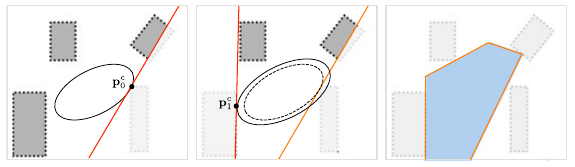
\includegraphics[width = 0.83\textwidth]{get_polyhedron.png}
  \caption{生成无碰撞无碰撞凸多面体示意图}
  \label{fig:get_polyhedron}
\end{figure}
如\figref{fig:get_polyhedron}所示,此过程也是通过一步步迭代,对之前生成的无碰撞椭球进行膨胀来得到最终的无碰撞凸多面体的,
具体流程见算法\ref{alg:generate_polyhedron}。
这里将第$i$步膨胀得到的半空间(halfspace)记作:
\begin{equation}
  H_i = \{\bm{p} \mid \trans{\bm{a}_i}\bm{p} < b_i\}
  \label{equ:halfspace_i}
\end{equation}

记最后得到的由$(m+1)$个半空间所确定的凸多面体为:
\begin{equation}
  \mathcal{P}(\bm{A}, \bm{b}) = \bigcap_{i=0}^m H_i = \{\bm{p} \mid \trans{\bm{A}}\bm{p} \prec \bm{b}\}, \bm{A} \in \mathbb{R}^{3\times m},\bm{b} \in \mathbb{R}^m
\end{equation}
\begin{algorithm}[h]
      \wuhao
      \caption{膨胀椭球生成无碰撞凸多面体\label{alg:generate_polyhedron}}  
      \begin{algorithmic}[1] %每行显示行号  
          \REQUIRE 无碰撞椭球$\xi^{0}(\bm{E},\bm{d})$,障碍物点集$O$ 
          \ENSURE 凸多面体$\mathcal{P}(\bm{A},\bm{b})$
          \STATE  $O_{remain}\gets \xi.getInside(O),j \gets 0$
    \WHILE {$O_{remain} \neq \emptyset$}
      \STATE $\bm{p}_{j}^{c} \gets \min_{\bm{q} \in O_{inside}}\Vert \bm{E}^{-1}(\bm{p}-\bm{d}) \Vert$ 
      \STATE 按比例膨胀$\xi^{0}$使其表面经过$\bm{p}_{j}^{c}$
      \STATE $\bm{a}_{j} \gets 2\bm{E}^{-1}\bm{E}^{-\text{T}}(\bm{p}_{j}^{c}-\bm{d})$
      \STATE $b_{j} \gets \bm{a}_{j}^{\text{T}}\bm{p}_{j}^{c}$
      \STATE 去除$O_{remain}$中不在半空间$H_{j}(\bm{a}_{j},b_{j})$之内的所有点
      \STATE $j \gets j+1$
    \ENDWHILE
    \STATE $\bm{A} \gets [\bm{a}_{0}\ \bm{a}_{1}\ \cdots]^{\text{T}}$,$\bm{b} \gets [b_0 \ b_1 \ \cdots]^{\text{T}}$
    \RETURN $\mathcal{P}(\bm{A},\bm{b})$
      \end{algorithmic}  
\end{algorithm} 

\subsection{效果展示}\label{subsec:impl_of_sfc_gen_algorithm}
如\figref{fig:sfc_generation}所示为SFC生成算法的运行结果的可视化示意图。
所使用的地图即是前述RRT测试所使用的宽松环境。
可以从图中清晰地看到每段路径周围的无碰撞椭球和在这些无碰撞椭球的基础上生成的凸多面体。
附近没有障碍物的路径段所生成的椭球保持初始的球形,而附近由障碍物的路径段所生成的椭球则被“压扁”;
所有凸多面体串成整个安全飞行走廊,注意这里加入了局部包围框(即一些额外的半空间),
以将飞行走廊限制在路径周围一定范围内。

在效率方面,该算法具有可观的计算速度,类似图中的飞行走廊的生成耗时在数十毫秒到百毫秒以内,
当然,耗时也会与点云中点的数量呈一定正相关。

\begin{figure}[!ht]
  \setlength{\subfigcapskip}{-1bp}
  \centering
  \begin{minipage}{\textwidth}

  \centering
  \subfigure{\label{fig:sfc_overview}}\addtocounter{subfigure}{-2}
  \subfigure{\subfigure[完整的SFC]{\includegraphics[width=0.3\textwidth]{octomap_sfc_overview.png}}}
  \hspace{0.2em}
  \subfigure{\label{fig:sfc_detail_1}}\addtocounter{subfigure}{-2}
  \subfigure{\subfigure[局部细节1]{\includegraphics[width=0.3\textwidth]{octomap_sfc_detail_1.png}}}
  \hspace{0.2em}
  \subfigure{\label{fig:sfc_detail_2}}\addtocounter{subfigure}{-2}
  \subfigure{\subfigure[局部细节2]{\includegraphics[width=0.3\textwidth]{octomap_sfc_detail_2.png}}}
  
  \end{minipage}
  \caption{SFC生成示意图}
  \label{fig:sfc_generation}
\end{figure}
\section{本章小结}\label{sec:summary_3}
本章首先对$SE(3)$空间中的RRT算法进行设计,
确定了$SE(3)$状态空间中的采样、插值和度量等操作,
介绍了用于近邻搜索的GNAT数据结构,
设计了基于点云地图和基于八叉树地图的两种有效性检测方法,
并对设计好的RRT算法进行了效果测试及分析;
随后设计并实现了安全飞行走廊的生成算法,并给出了实测效果。
综上所述,本章完成了对轨迹规划前端算法的设计与实现,
为后端部分提供了可行路径和安全约束等初始信息。


% 第4章
% !TEX root = ../main.tex

% 中英标题:\chapter{中文标题}[英文标题]
\chapter{后端轨迹生成算法设计}\label{chap:back_end_trajectory_generation}

\section{引言}\label{sec:intro_4}
上一章设计了轨迹规划的前端算法,
为本章所介绍的轨迹规划后端部分提供了数据输入。
后端部分的主要任务是根据前端生成的初始可行路径或安全飞行走廊,
通过拟合、优化的方法得到一条具备时间律的连续、平滑且安全的轨迹输入到飞行器的控制器中。
本章介绍基于优化的后端轨迹生成算法设计,
\ref{sec:geometrically_constrained_trajectory_optimization}节介绍几何约束下多旋翼的轨迹优化原理;
\ref{sec:geometrically_constrained_SE3_planning_for_omnihex}节基于该原理构建了几何约束下过驱动飞行器6自由度$SE(3)$轨迹优化框架,
并提出了该框架下使用欧拉角和使用四元数表示姿态的两种规划方式,并推导了相应公式。

\section{几何约束下多旋翼的轨迹优化原理}\label{sec:geometrically_constrained_trajectory_optimization}
几何约束下多旋翼的轨迹优化框架GCOPTER\cite{2021Geometrically}由Wang等人于2021年提出,
该框架在对多旋翼无人机施加复杂的安全约束、苛刻的动力学约束以及自定义需求的情况下依然能保证极高的计算效率和轨迹质量,
其优秀性能催生了许多优秀成果\cite{2021Fast, zhou2022swarm}。

GCOPTER论文的主要贡献概括为以下几点:
\begin{enumerate}
  \renewcommand{\labelenumi}{(\theenumi)}
  \item 给出了多阶段控制代价(control effort)最小化问题的最优充要条件,并基于此条件设计了最小控制代价轨迹类MINCO;
  \item 使用数学技巧消去轨迹时间分配的约束和中间点的空间空间约束;\label{itm:eliminate_geometric_constraints}
  \item 构造时间积分罚函数软化连续时间约束;\label{itm:time_int_penalty}
  \item 利用\ref{itm:eliminate_geometric_constraints}和\ref{itm:time_int_penalty}化约束优化问题为无约束优化问题,使用拟牛顿法(quasi-Newton methods)高效求解。
\end{enumerate}
本课题期望将此框架扩展到过驱动飞行器的6自由度$SE(3)$轨迹规划中,下面先对框架原理进行详细介绍。

\subsection{问题形式}\label{subsec:problem_formulation}
多旋翼无人机等微分平坦机器人的轨迹规划任务常常在其平坦输出空间中进行,
所期望得到的结果是一条平坦输出$\bm{z}$的轨迹$\bm{z}(t):[0, T]\mapsto\mathbb{R}^m$,
对于OmniHex这样的全驱动多旋翼飞行器而言有$m=6$。

GCOPTER的优化目标是在满足一定的几何约束和连续时间约束的前提下使轨迹尽量平滑且尽量满足设定的时间分配要求,
这个目标通过最小化时间正则化的导数平方积分控制代价来实现。
几何约束包括构型空间中的空间约束,代表飞行器可以处于的安全区域,表达为:
\begin{equation}
  \bm{z}(t) \in \mathcal{F}, \forall t \in  [0, T] \label{equ:spatial_constraints_in_c_space}
\end{equation}
其中$\mathcal{F}$为构型空间(平坦输出空间)中的无障碍物区域。
连续时间约束包含其他对飞行器状态$\bm{x}(t)$和控制输入$\bm{u}(t)$的所有约束,如动力学限制、其他与特定任务相关约束等。
所有这些自定义约束记为:
\begin{equation}
  \mathcal{G}_D(\bm{x}(t), \bm{u}(t)) \preceq \textbf{0}, \forall t \in [0, T]
  \label{equ:constraints_on_x_and_u}
\end{equation}
利用微分平坦关系可以将$\mathcal{G}_D$转化为对平坦输出及其有限阶导数的约束(\figref{fig:constraint_transformation}): 
\begin{equation}
  \mathcal{G}(\bm{z}(t), \dot{\bm{z}}(t), \cdots, \bm{z}^{(s)}(t)\}) \preceq \textbf{0}, \forall t \in [0, T]
  \label{equ:constraints_on_z}
\end{equation}
其中$\mathcal{G}$包含$n_g$个约束。

假设要最小化平方积分的导数阶数为$s \in \mathbb{N}_+$,
即取$\bm{v} = \bm{z}^{(s)}$,并记:
\begin{gather}
  \bm{z}^{[s-1]} = \trans{\left[\trans{\bm{z}} \  \trans{\dot{\bm{z}}} \  \cdots \trans{\bm{z}^{(s-1)}} \right]} \in \mathbb{R}^{ms} \label{equ:derivative_vector_of_z} \\
  \bm{z}_i^{[s-1]} = \trans{\left[ z_i \ \dot{z}_i \ \cdots z_i^{(s-1)} \right]} \in \mathbb{R}^{s} \label{equ:derivative_vector_of_zi}
\end{gather}
则整个轨迹优化过程即为求解下述约束优化问题:
\begin{subeqnarray}
  \label{equ:constrained_optimization}
  &\min_{\bm{z}(t), T} &\int_0^T \trans{\bm{v}(t)}\bm{v}(t)\text{d}t + \rho(T) \slabel{equ:time_regularized_control_effort} \\
  &s.t. &\bm{v}(t) = \bm{z}^{(s)}(t), \forall  t \in [0, T], \\
  & & \mathcal{G}(\bm{z}(t), \dot{\bm{z}}(t), \cdots, \bm{z}^{(s)}(t)\}) \preceq \textbf{0}, \forall t \in [0, T], \\
  & & \bm{z}(t) \in \mathcal{F}, \forall t \in  [0, T], \\ 
  & & \bm{z}^{[s-1]}(0) = \bar{\bm{z}}_o, \bm{z}^{[s-1]}(T) = \bar{\bm{z}}_f. \slabel{equ:boundary_conditions}
\end{subeqnarray}
其中$\rho(T)$为时间正则项,它代表了轨迹总时间所期望满足的性质,是控制代价与总时间之间的权衡。
例如,如果希望飞行器尽快到达重点,即总时间越$T$短越好,那么可取为$\rho_s(T) = k_\rho T$;
如果希望轨迹总时间尽可能接近给定的期望值$T_{\Sigma}$,那么可取为$\rho_s(T) = k_\rho (T - T_{\Sigma})^2$;
如果希望$T$严格固定为$T_{\Sigma}$,则可取为:
\begin{equation}
  \rho_f(T) = 
  \begin{cases}
    0 \quad &if \  T = T_{\Sigma} \\
    \infty \quad &if \ T \neq T_{\Sigma}
  \end{cases}
  \label{equ:fixed_time_regularization_term}
\end{equation}

\subsection{最优性条件与MINCO轨迹类}\label{subsec:optimal_condition_and minco_trajectory}
为了使轨迹更容易地满足安全约束和动力学约束,通常将平坦输出轨迹$\bm{z}(t)$表示为分段多项式,
一条$k$阶$M$段分段多项式轨迹形式如下:
\begin{equation}
  \bm{z}(t) = \trans{\bm{c}_i}\bm{\beta}(t - t_{i-1}), t \in [t_{i-1}, t_i], i = 1, 2, \cdots, M
  \label{equ:piecewise_polynomial_trajectory} 
\end{equation}
其中$\bm{c}_i \in \mathbb{R}^{(k+1) \times m}$为第$i$段多项式的系数矩阵,
$\bm{\beta}(t) = \left[1 \  t \  \cdots \  t^N\right] \in \mathbb{R}^{(k+1)}$为多项式基底。

先不考虑约束$\mathcal{F}$和$\mathcal{G}$以及时间正则项$\rho(T)$,考虑如下$M$阶段控制代价最小化问题:
\begin{subeqnarray}
  \label{equ:unconstrained_multistage_optimal_control_problem}
  &\min_{\bm{z}(t)} &\int_{t_0}^{t_M} \trans{\bm{v}(t)}\bm{v}(t)\text{d}t \slabel{equ:control_effort} \\
  &s.t. &\bm{v}(t) = \bm{z}^{(s)}(t), \forall t \in [t_0, t_M], \\
  & & \bm{z}^{[s-1]}(0) = \bar{\bm{z}}_o, \bm{z}^{[s-1]}(T) = \bar{\bm{z}}_f, \slabel{equ:intermediate_conditions_moc}\\
  & & \bm{z}^{[d_i-1]}(t_i) = \bar{\bm{z}}_i, i = 1, 2, \cdots, M-1, \slabel{equ:boundary_conditions_moc}\\
  & & t_{i-1} < t_i, i = 1, 2, \cdots, M. \slabel{equ:temporal_non_negative_constraints}
\end{subeqnarray}
在这个问题中,时间段$[t_0, t_M]$被$(M+1)$个固定的时间戳$ t_1, \cdots, t_{M-1}  $分割成$M$段;
此外,在每段的终点$t_i$处平坦输出的前$d_i - 1 < s$阶导数也被固定为$\bm{z}_i \in \mathbb{R}^{md_i}$。
在GCOPTER的论文中给出了多阶段最优控制问题\equref{equ:unconstrained_multistage_optimal_control_problem}的最优充要条件:
\begin{theorem}[(最优充要条件)]
  \label{thr:optimality_conditions}
  优化问题\equref{equ:unconstrained_multistage_optimal_control_problem}存在唯一一个最优解$\bm{z}^*(t):[t_0, t_M] \mapsto \mathbb{R}^m$;
  且轨迹$\bm{z}$是优化问题\equref{equ:unconstrained_multistage_optimal_control_problem}的最优解,
  当且仅当如下条件同时成立:
  \begin{enumerate}
    \renewcommand{\labelenumi}{(\theenumi)}
    \item $\bm{z}^*(t):[t_0, t_M] \mapsto \mathbb{R}^m$是一个$(2s-1)$次多项式,$1 \leq i \leq M$;
    \item $\bm{z}^*(t)$满足\equref{equ:boundary_conditions_moc}所示的边界条件;
    \item $\bm{z}^*(t)$满足\equref{equ:intermediate_conditions_moc}所示的中间条件;
    \item 对任意的$i = 1, \cdots, M-1$,$\bm{z}^*(t)$在$t_i$处$\bar{d}_i-1$阶连续可微,其中处$\bar{d}_i=2s-d_i$。
  \end{enumerate}
\end{theorem}
利用这个最优充要条件,就可以无需计算代价泛函,以$O(M)$的时间复杂度求出这条最优轨迹。

记\equref{equ:unconstrained_multistage_optimal_control_problem}的最优轨迹$\bm{z}^*(t)$的总系数矩阵为;
\begin{equation}
  \bm{c} = \trans{
    \begin{bmatrix}
      \trans{\bm{c}_1} & \cdots & \trans{\bm{c}_1}
    \end{bmatrix}
  } \in \mathbb{R}^{2Ms \times m}
  \label{equ:coeff_matrix_of_the_whole_traj} 
\end{equation}
时间分配向量记为:
\begin{equation}
  \bm{T} = \trans{
    \begin{bmatrix}
      t_1 - t_0 & \cdots & t_M - t_{M-1}
    \end{bmatrix}
  } = \trans{
    \begin{bmatrix}
      T_1 & \cdots & T_M
    \end{bmatrix}
  } \in \mathbb{R}_+^{M}
  \label{equ:time_alloc_vector}
\end{equation}
记\equref{equ:unconstrained_multistage_optimal_control_problem}中的边界条件为$\bm{D}_0, \bm{D}_M \in \mathbb{R}^{s \times m}$,
中间条件为$\bm{D}_i \in \mathbb{R}^{d_i \times m}$,
这样根据定理\ref{thr:optimality_conditions}中关于中间时刻$t_i$处导数的取值条件和连续性条件可以写为下式:
\begin{equation}
  \begin{bmatrix}
    \bm{E}_i & \bm{F}_i
  \end{bmatrix}
  \begin{bmatrix}
    \bm{c}_i \\ \bm{c}_{i+1}
  \end{bmatrix} =
  \begin{bmatrix}
    \bm{D}_i \\ \textbf{0}_{\bar{d}_i \times m}
  \end{bmatrix}, 
  i = 1, 2, \cdots, M-1
  \label{equ:conditons_at_t_i}
\end{equation}
其中$E_i,F_I \in \mathbb{R}^{2s \times 2s}$,且有:
\begin{gather}
  \bm{E}_i = \trans{
    \begin{bmatrix}
      \bm{\beta}(T_i) & \cdots & \bm{\beta}^{(d_i-1)}(T_i) & \bm{\beta}(T_i) & \cdots & \bm{\beta}^{(\bar{d}_i-1)}(T_i)
    \end{bmatrix}
  } \label{equ:E_i}\\
  \bm{F}_i = \trans{
    \begin{bmatrix}
      \textbf{0} & -\bm{\beta}(0) & \cdots & -\bm{\beta}^{(\bar{d}_i-1)}(0)
    \end{bmatrix}
  }
  \label{equ:F_i}
\end{gather}
特别地,定义$\bm{F}_0,\bm{E}_M \in \mathbb{R}^{s \times 2s}$为:
\begin{gather}
  \bm{F}_0 = \trans{
    \begin{bmatrix}
      \bm{\beta}(0) & \cdots & \bm{\beta}^{(s-1)}(0)
    \end{bmatrix}
  } \label{equ:F_0}\\
  \bm{E}_M = \trans{
    \begin{bmatrix}
      \bm{\beta}(T_M) & \cdots & \bm{\beta}^{(s-1)}(T_M)
    \end{bmatrix}
  }
  \label{equ:E_M}
\end{gather}
于是,根据定理\ref{thr:optimality_conditions}可构造出关于最优轨迹系数矩阵$\bm{c}$的线性方程组:
\begin{equation}
  \bm{Mc} = \bm{b}
  \label{equ:linear_equation_system_wrt_c}
\end{equation}
其中$\bm{M} \in \mathbb{R}^{2Ms \times 2Ms}$仅与时间分配向量$\bm{T}$有关,具有带状结构;
$\bm{b} \in \mathbb{R}^{2Ms \times m}$仅与中间条件有关。
二者形式如下:
\begin{gather}
  \bm{M} = 
    \begin{bmatrix}
      \bm{F}_0 & \textbf{0} & \textbf{0} & \cdots & \textbf{0} \\
      \bm{E}_1 & \bm{F}_1 & \textbf{0} & \cdots & \textbf{0} \\
      \textbf{0} & \bm{E}_2 & \bm{F}_2 & \cdots & \textbf{0} \\ 
      \vdots & \vdots & \vdots & \ddots & \vdots \\
      \textbf{0} & \textbf{0} & \textbf{0} & \cdots & \bm{F}_{M-1} \\
      \textbf{0} & \textbf{0} & \textbf{0} & \cdots & \bm{E}_{M}
    \end{bmatrix}
   \label{equ:M} \\
  \bm{b} = \trans{
    \begin{bmatrix}
      \bm{D}_0^{\text{T}} & \bm{D}_1^{\text{T}} & \textbf{0}_{m \times \bar{d}_i} & 
      \cdots & \bm{D}_{M-1}^{\text{T}} & \textbf{0}_{m \times \bar{d}_{M-1}} & \bm{D}_{M}^{\text{T}}
    \end{bmatrix}
  } \label{equ:b}
\end{gather}

由最优解的存在性和唯一性,可以保证$\bm{M}$的非奇异性,
然后利用带状矩阵的PLU分解就可以以$O(M)$的线性时间和空间复杂度求解出$\bm{c}$;
同时对任意的时间分配、边界条件和中间条件,$\bm{M}$和$\bm{b}$均可以以线性复杂度构建。
这样,通过直接应用定理\ref{thr:optimality_conditions},
无需代价泛函即可用极低的复杂度得到多阶段最优控制问题\equref{equ:unconstrained_multistage_optimal_control_problem}的最优解。
需要注意的是,
如果在算法实现时采用的时直接LU分解,那么需要调整$\bm{M}$和$\bm{b}$中行的顺序来避免主对角线上出现0。

对于多旋翼飞行器来说,飞行轨迹的安全性通常决定于它的空间特性,而动力学限制通常决定于它的时间属性,
因此将轨迹参数分为两组:
第一组包含轨迹必须通过的中间点;第二组包含轨迹中不同片段的时间分配向量。
基于这些参数,利用定理\ref{thr:optimality_conditions}即可得到轨迹的系数矩阵$\bm{c}$,
这个系数矩阵对应的就是在给定的阶数、时间分配和中间条件下具有最小控制量的轨迹,
若$s=4$,那么得到的就是Mellinger等人提出的最小化加加加速度轨迹\cite{2011minimumsnap}.
Wang等人将这类以中间点和时间分配为参数,使用定理\ref{thr:optimality_conditions}构建出的轨迹称作MINCO轨迹\cite{2021Geometrically}。

记中间点为$\bm{q} = \begin{bmatrix} \bm{q}_1 & \cdots & \bm{q}_{M-1} \end{bmatrix} \in \mathbb{R}^{m \times (M-1)}$,
$\bm{q}_i \in \mathbb{R}^m$为指定在$t_i$时刻的中间条件($d_i-1=0$),
则MINCO轨迹定义为$\mathscr{T}_{\text{MINCO}}$定义为
\begin{equation}
  \mathscr{T}_{\text{MINCO}} \overset{\text{def}}{=} 
  \{
    \bm{p}(t):[t_0, t_M] \mapsto \mathbb{R}^m \mid \bm{c} = \bm{c}(\bm{q}, \bm{T}), \forall \bm{q} \in \mathbb{R}^{m \times (M-1)}, \bm{T} \in \mathbb{R}_+^{M}
  \}
  \label{equ:definition_of_minco}
\end{equation}
其中$\bm{c}(\bm{q}, \bm{T})$即是由定理\ref{thr:optimality_conditions}决定的整条轨迹的系数矩阵,
这样轨迹的参数就由系数转化为了$\bm{q}$和$\bm{T}$,实现了参数降维.

\begin{figure}[ht]
  \centering
  \includegraphics[width = 0.58\textwidth]{minco.png}
  \caption{MINCO轨迹的空间变形示意图}
  \label{fig:minco}
\end{figure}

现在如果有约束存在,
则调整$\bm{q}$就可以对$\mathscr{T}_{\text{MINCO}}$进行空间上的变形,使整条轨迹不与障碍物发生碰撞(\figref{fig:minco});
调整$\bm{T}$则可以对$\mathscr{T}_{\text{MINCO}}$进行时间上的变形,使之满足动力学限制。
GCOPTER框架就是通过MINCO的时空变形来优化目标函数,从而得到一条给定需求下的最优轨迹。

\subsection{MINCO轨迹类中的梯度计算}\label{subsec:gradient_calculation_in_minco}
上小节提到,基于MINCO的轨迹优化框架通过调整轨迹参数$\bm{q}$和$\bm{T}$来优化给定的目标函数。
及自定义的轨迹优化优化目标函数为一个二阶连续可微的标量函数$F(\bm{c}, \bm{T})$,且其梯度已知,
那么这个目标函数在$\mathscr{T}_{\text{MINCO}}$中可以计算如下:
\begin{equation}
  H(\bm{q}, \bm{T}) = F(\bm{c}(\bm{q}, \bm{T}), \bm{T})
  \label{equ:objective_form_in_minco}
\end{equation}

在对目标函数进行优化时,通常需要用到其梯度信息,
即需要计算${\partial H}/{\partial \bm{q}}$和${\partial H}/{\partial \bm{T}}$。
显然计算$H$的值与求解$\mathscr{T}_{\text{MINCO}}$中任意一条轨迹(即计算$\bm{c}(\bm{q}, \bm{T})$)具有相同的复杂度$O(M)$,
下面介绍从已知的${\partial F}/{\partial \bm{c}}$和${\partial F}/{\partial \bm{T}}$计算${\partial H}/{\partial \bm{q}}$和${\partial H}/{\partial \bm{T}}$的线性复杂度方法。

首先给出如下结论,这里省去推导过程:
\begin{equation}
  \pdiff{H}{\bm{q}_i} = \trans{\left(\bm{M}^{-\text{T}}\pdiff{F}{\bm{c}}\right)} \bm{e}_{(2i-1)s+1}
  \label{equ:grad_H_qi}
\end{equation}
其中$\bm{e}_j$代表单位矩阵$\bm{I}_{2Ms}$的第$j$列。
计算过程中需要对$\trans{\bm{M}}$求逆,直接的求逆运算具有$O(M^3)$的时间复杂度。
注意到先前求解$\bm{c}$时对$\bm{M}$进行了PLU分解,可以利用这里的结果来避免求逆,减小复杂度。
令\equref{equ:grad_H_qi}中括号中表达式的结果为$\bm{G}\in\mathbb{R}^{2Ms\times m}$,
则得到关于$\bm{G}$的线性方程组: 
\begin{equation}
  \trans{\bm{M}}\bm{G} = \pdiff{F}{\bm{c}}
  \label{equ:linear_equation_system_wrt_G}
\end{equation}
记$M$的PLU分解结果为$\bm{M} = \bm{PLU}$,则$\trans{\bm{M}}$也存在PLU分解,有$\trans{\bm{M}}=\bar{\bm{L}}\bar{\bm{U}}\trans{\bm{P}}$,其中 
\begin{equation}
  \bar{\bm{L}} = \trans{\bm{U}}(\bm{U}\circ\bm{I})^{-1}, \bar{\bm{U}} = (\bm{U}\circ\bm{I})\trans{\bm{L}}
  \label{equ:LU_of_trans_M}
\end{equation}
其中需要求逆的只是一个对角矩阵,符号$\circ$为矩阵的Hadamard乘积。
那么现在就可以用线性复杂度求出$\bm{G}$了,
为方便起见,将$\bm{G}$写成如下分块形式:
\begin{equation}
  \bm{G} = \trans{
    \begin{bmatrix}
      \bm{G}_0^{\text{T}} & \bm{G}_1^{\text{T}} & \cdots & \bm{G}_{M-1}^{\text{T}} & \bm{G}_M^{\text{T}}
    \end{bmatrix}
  }
  \label{equ:block_form_of_G}
\end{equation}
其中$\bm{G}_0, \bm{G}_M \in \mathbb{R}^{s \times m}$而$\bm{G}_i \in \mathbb{R}^{2s \times m}, i = 1, 2, \cdots, M-1$。
这样$H$对$\bm{q}$的梯度就可以写为:
\begin{equation}
  \pdiff{H}{\bm{q}} = 
  \begin{bmatrix}
    \bm{G}_1^{\text{T}}\bm{e}_1 & \cdots & \bm{G}_{M-1}^{\text{T}}\bm{e}_1
  \end{bmatrix}
  \label{equ:grad_H_q}
\end{equation}
相似地可以得到$H$对$T_i$的梯度: 
\begin{equation}
  \pdiff{H}{T_i} = \pdiff{F}{T_i} - \text{tr}\{\bm{G}_i^{\text{T}}\pdiff{\bm{E}_i}{T_i}\bm{c}_i\}
  \label{equ:grad_H_Ti}
\end{equation}

\subsection{几何约束的消去}\label{subsec:elimination_of_geometric_constraints}
在MINCO轨迹类中,进行时空变形可使轨迹在满足可行性约束的同时保持局部光滑性。
基于$\mathscr{T}_{\text{MINCO}}$的轨迹优化问题的形式如下:
\begin{subeqnarray}
  \label{equ:optimization_in_minco}
  &\min_{\bm{q}, \bm{T}} &J(\bm{q}, \bm{T}) = J_q(\bm{q}, \bm{T}) + \rho(\Vert\bm{T}\Vert_1) \slabel{equ:time_regularized_control_effort_in_minco} \\
  &s.t. \ &\mathcal{G}(\bm{z}(t), \dot{\bm{z}}(t), \cdots, \bm{z}^{(s)}(t)) \preceq \textbf{0}, \forall t \in [0, T], \slabel{equ:time_continuos_constraint_minco}\\
  & & \bm{q}_i \in \mathcal{P}_i, i = 1, 2, \cdots, M-1, \slabel{equ:spatial_constraints_minco}\\ 
  & & \bm{T} \succ \textbf{0}, \slabel{equ:temporal_constraints_minco}\\
  & & \bm{z}^{[s-1]}(0) = \bar{\bm{z}}_o, \bm{z}^{[s-1]}(T) = \bar{\bm{z}}_f. \slabel{equ:boundary_conditions_minco}
\end{subeqnarray}
其中$J_q(\bm{q}, \bm{T}):=J_c(\bm{c}, \bm{T})$,$J_c(\bm{c}, \bm{T})$为由轨迹多项式系数和时间分配确定的控制代价,
具有解析的表达式和梯度\cite{2021Geometrically};$\mathcal{P}_i$为第$i$个中间点$\bm{q}_i$所被分配到的SFC凸多面体。

几何约束\equref{equ:spatial_constraints_minco}和\equref{equ:temporal_constraints_minco}是必要的,
但会在一定程度上影响优化速度
下面介绍消去几何约束使时空变形免受不等式约束组合困难(combinatorial difficulty)的限制的方法。
\subsubsection{时间约束的消去}\label{subsubsec:elimination_of_temporal_constraints}
对时间分配向量$\bm{T}$的两种约束会对带约束优化过程产生不利影响:
\begin{enumerate}
  \renewcommand{\labelenumi}{(\theenumi)}
  \item 如\equref{equ:temporal_constraints_minco}所示的那样,要求$\bm{T}$中的每个元素都大于0,
        这是由实际意义决定的,并且如\figref{fig:influence_of_temporal_constraints}所示,当
        $\bm{T}$中的任意一个元素在优化过程中接近于0时,都会导致$J_q$趋向于无穷大,因为$\bm{q}$中不存在两个相邻且相同的点;
  \item 如\figref{fig:influence_of_temporal_constraints}所示, 
        当$\rho=\rho_f$时,会加入一个额外的约束$\sum_{i = 1}^{M-1}T_i < T_{\Sigma}$,使得$\bm{T}$的可行区域进一步缩减。
\end{enumerate}

在上述两种情况下,病态的Hessian矩阵以及可行域边界处出现的不可行搜索步长都会拖慢优化过程的收敛。
在GCOPTER中,采取微分同胚映射(diffeomorphism)的手段来消去上述时间约束。
\begin{figure}[ht]
  \centering
  \includegraphics[width = 0.58\textwidth]{influence_of_temporal_constraints.png}
  \caption{时间约束示意图}
  \label{fig:influence_of_temporal_constraints}
\end{figure}

对于要求总时间严格固定,即$\rho=\rho_f$的情形,$\bm{T}$的可行域描述为如下集合:
\begin{equation}
  \mathcal{T}_f = \{
    \bm{T} \in \mathbb{R}_+^M \mid \Vert\bm{T}\Vert_1 = T_{\Sigma}
  \}
  \label{equ:feasible_domain_of_T_fixed_tt}
\end{equation}
那么可以证明$\mathcal{T}_f$与$\mathbb{R}^{M-1}$是微分同胚的,
其中一个$C^{\infty}$的微分同胚映射如\equref{equ:diffeophism_T_fixed_tt}所示
\begin{subeqnarray}
  \label{equ:diffeophism_T_fixed_tt}
  &T_i = \frac{e^{\tau_i}}{1 + \sum_{j=1}^{M-1}e^{\tau_j}}T_{\Sigma}, i = 1, 2, \cdots, M-1, \slabel{equ:diffeophism_T_fixed_tt_1} \\ 
  &T_M = T_{\Sigma} - \sum_{i=1}^{M-1}T_i \slabel{equ:diffeophism_T_fixed_tt_2}
\end{subeqnarray}
利用这个映射,把目标变量由受约束的$\bm{T}$转化为自由变量$\bm{\tau}$,
这样就摆脱了可行域边界附近的不利条件,且此时时间正则项恒为0。
若令${\partial J_q}/{\partial \bm{T}} = [\bm{g}_a^{\text{T}} \  g_b]^{\text{T}}$,
则$J$对$\bm{\tau}$的梯度如下式所示:
\begin{equation}
  \pdiff{J}{\bm{\tau}} = 
  \left(
  \frac{(\bm{g}_a - g_b \cdot \textbf{1}) \circ e^{[\bm{\tau}]}}{1 + \Vert e^{[\bm{\tau}]} \Vert_1} - 
  \frac{(\bm{g}_a^{\text{T}}e^{[\bm{\tau}]} - g_b\Vert e^{[\bm{\tau}]} \Vert_1)e^{[\bm{\tau}]}}{(1 + \Vert e^{[\bm{\tau}]} \Vert_1)^2}
  \right)T_{\Sigma}
  \label{equ:grad_J_tau}
\end{equation}
其中$e^{[\cdot]}$表示向量$\cdot$按元素求指数函数值。
那么可以看到,由$\bm{\tau}$正向计算$J$以及反向计算梯度仍然只需要$O(M)$的时间和空间复杂度。
对于总时间不严格固定,即$\rho=\rho_s$的情形,
可以用$\bm{T}=e^{[\bm{\tau}]}$作为从$\mathbb{R}^M$到作为从$\mathbb{R}_+^M$的微分同胚映射,
注意此时在计算目标函数值和梯度时需要加上时间正则项。

可以证明,上述变换不会抹去$J$原有的局部最小值点,也不会引入额外的局部最小值点。

\subsubsection{空间约束的消去}\label{subsubsec:elimination_of_spatial_constraints}
对于\equref{equ:spatial_constraints_in_c_space}所示的空间约束,
要求对整条轨迹上的点都成立。
对于由凸多面体组成的复杂空间约束,这个要求通过两个阶段来实现:
(1)按顺序将中间点分配到组成安全飞行走廊的凸多面体中,如\equref{equ:spatial_constraints_minco}所示;
(2)在给定分辨率下使整条轨迹满足空间约束。
本小节处理阶段(1),阶段(2)的处理将在\ref{subsec:processing_of_continuous_time_constraints}小节介绍。

\begin{figure}[ht]
  \centering
  \includegraphics[width = 0.7\textwidth]{polyhedron_constraint_elimination.png}
  \caption{凸多面体约束转化示意图}
  \label{fig:transformation_of_polyhedron_constraints}
\end{figure}

记一个$\mathbb{R}^n$中的凸多面体$\mathcal{P}$的$(\hat{n}+1)$个顶点为$[\bm{v}_0 \ \cdots \ \bm{v}_{\hat{n}}]$,
记$\hat{\bm{v}}_i = \bm{v}_i - \bm{v}_0$,及$\hat{\bm{V}} = [\hat{\bm{v}}_1 \ \cdots \ \hat{\bm{v}}_{\hat{n}}]$,
这样每一个中间点$\bm{q}\in\mathbb{R}^n$在重心坐标系(barycentric coordinate system)下就可以表示为:
\begin{equation}
  \bm{q} = \bm{v}_0 + \hat{\bm{V}}\bm{w}
  \label{equ:q_in_barycentric_coordinate}
\end{equation}
其中$\bm{w} = \trans{[w_1 \ \cdots \ w_{\hat{n}}]}\in\mathbb{R}^{\hat{n}}$为重心坐标的后$\hat{n}$个元素。
凸多面体$\mathcal{P}$内的每一个点对应的$\bm{w}$构成的点集是$\mathbb{R}^{\hat{n}}$中的标准单纯形(standard simplex):
\begin{equation}
  \mathcal{P}_w^{\hat{n}} = \{
    \bm{w} \in \mathbb{R}^{\hat{n}} \mid \bm{w} \succeq \textbf{0}, \Vert \bm{w} \Vert_1 \leq 1
  \}
  \label{equ:standard_simplex}
\end{equation}
这样凸多面体$\mathcal{P}$就可以用V-表示法表达为:
\begin{equation}
  \mathcal{P} = \{
    \bm{v}_0 + \hat{\bm{V}}\bm{w} \mid \bm{w} \in \mathcal{P}_w^{\hat{n}}
  \}
  \label{equ:V_polyhedron}
\end{equation}

换句话说,凸多面体约束$\bm{q} \in \mathcal{P}$实际上被转化为了一个$\mathbb{R}^{\hat{n}}$中的标准单纯形约束$\bm{w} \in \mathcal{P}_w^{\hat{n}}$(\figref{fig:transformation_of_polyhedron_constraints})。
此单纯形约束还可以进一步用非线性变换消去:
首先用按元素的平方变换$\bm{w}=[\bm{x}]^2,\forall x\in\mathbb{R}^{\hat{n}}$消去非负约束,
这样单纯形约束$\bm{w} \in \mathcal{P}_w^{\hat{n}}$转化为了球约束$\bm{x}\in\mathcal{B}^{\hat{n}}$,其中:
\begin{equation}
  \mathcal{B}^{\hat{n}} = \{ 
    \bm{x} \in \mathbb{R}^{\hat{n}} \mid \Vert \bm{x} \Vert_2 \leq 1
  \}
  \label{equ:ball_constraint}
\end{equation}
\begin{figure}[ht]
  \centering
  \includegraphics[width = 0.62\textwidth]{ball_constraint_elimination.png}
  \caption{球约束消去示意图}
  \label{fig:elimination_of_ball_constraints}
\end{figure}
然后再如\figref{fig:elimination_of_ball_constraints}所示使用逆球极投影(inverse stereographic projection)变换和一个正交投影变换可以消去球约束,
最后得到一个从整个$\mathbb{R}^{\hat{n}}$到凸多面体$\mathcal{P}$的映射:
\begin{equation}
  f_{\mathcal{H}}(\bm{\xi}) = \bm{v}_0 + \frac{4\hat{\bm{V}}[\bm{\xi}]^2}{(\trans{\bm{\xi}}\bm{\xi} + 1)^2} \in \mathcal{P}, 
  \forall \bm{\xi} \in \mathbb{R}^{\hat{n}}
  \label{equ:polyhedron_constraint_elimination_map}
\end{equation}
当$\bm{\xi}$在整个$\mathbb{R}^{\hat{n}}$中自由运动时,
经由映射$f_{\mathcal{H}}$得到的$\mathbb{R}^n$中的像始终位于凸多面体$\mathcal{P}$内。
这样,与时间约束类似,用凸多面体表示的空间约束被用引入新的目标变量$\bm{\xi}$的方式消去了。
在优化过程开始之前会给定的初始$\bm{q}_i$,其对应的初始$\bm{\xi}_i$可以通过最小化$\Vert \bm{f}_{\mathcal{H}}(\bm{\xi}_i) - \bm{q}_i \Vert_2^2$的值来得到。


若记${\partial J}/{\partial \bm{q}_i}=\bm{g}_i$,则$J$关于对应的$\bm{\xi}_i$的梯度就可以写为:
\begin{equation}
  \pdiff{J}{\bm{\xi}_i} = 
  \frac{8\bm{\xi}_i \circ \trans{\hat{\bm{V}}}\bm{g}_i}{(\bm{\xi}_i^{\text{T}}\bm{\xi}_i+1)^2} - 
  \frac{16\bm{g}_i^{\text{T}}\hat{\bm{V}}[\bm{\xi}]^2}{(\bm{\xi}_i^{\text{T}}\bm{\xi}_i+1)^3}\bm{\xi}_i
  \label{equ:grad_J_xii}
\end{equation}

上述变换同样不会抹去$J$原有的局部最小值点,也不会引入额外的局部最小值点。

\subsection{连续时间约束$\mathcal{G}$的处理}\label{subsec:processing_of_continuous_time_constraints}
\equref{equ:time_continuos_constraint_minco}表达的连续时间$\mathcal{G}$约束包含无穷多个不等式约束,计算机难以处理。
GCOPTER中使用时间积分罚函数(time integral penalty function)法来处理$\mathcal{G}$,
通过对约束越界量的积分,将$\mathcal{G}$软化为了目标函数的一部分。

对任意一条轨迹$\bm{z}(t):[0, T] \mapsto \mathbb{R}^m$,定义:
\begin{equation}
  \bm{I}_{\mathcal{G}}^k[\bm{z}] \overset{\text{def}}{=} 
  \int_0^T \bm{K}(\mathcal{G}(\bm{z}(t), \cdots, \bm{z}^{(s)}(t))) \text{d}t
  \label{equ:time_int_violation}
\end{equation}
其中$k\in\mathbb{R}_+$,$\bm{K}(\cdot)=\max[\cdot,\textbf{0}]^k$代表先按行与0比较取最大值组成最大值向量,
然后将最大值向量按元素取$k$次幂。那么轨迹$\bm{z}$的时间积分罚函数定义为:
\begin{equation}
  I_{\mathcal{G}}[\bm{z}] \overset{\text{def}}{=} 
  \trans{\bm{\chi}}\bm{I}_{\mathcal{G}}^3[\bm{z}]
  \label{equ:form_of_tipf}
\end{equation}
其中$\bm{\chi}\in\mathbb{R}_{\geq}^{n_g}$为惩罚权重向量,令$k=3$可以保证罚函数的二阶可微性。
通常惩罚权重的元素应该足够大,这样如果没有约束被打破,罚函数值将保持为0;
而一旦$\bm{z}(t)$的某个部分打破了约束,罚函数值就会急剧增加。
通过把$I_{\mathcal{G}}[\bm{z}]$作为一项加入目标代价函数,
优化后的轨迹将会倾向于满足连续时间约束$\mathcal{G}$。

由于计算机无法直接处理连续函数,故使用数值积分的方式计算罚函数$I_{\mathcal{G}}[\bm{z}]$的值。
定义采样函数$\mathcal{G}_v:\mathbb{R}^{2s\times m}\times \mathbb{R}_+ \times [0,1] \mapsto \mathbb{R}^{n_g}$为:
\begin{equation}
  \mathcal{G}_v(\bm{c}_i, T_i, \hat{t}) = 
  \mathcal{G}\left( 
    \bm{c}_i^{\text{T}}\bm{\beta}(T_i\cdot \hat{t}), \cdots, \bm{c}_i^{\text{T}}\bm{\beta}^{(s)}(T_i\cdot \hat{t})
  \right)
  \label{equ:sample_function}
\end{equation}
则第$i$段轨迹的数值积分$I_i:\mathbb{R}^{2s\times m}\times \mathbb{R}_+ \times \mathbb{N} \mapsto \mathbb{R}_+$为:
\begin{equation}
  I_i(\bm{c}_i, T_i, \kappa_i) = \frac{T_i}{\kappa_i} \sum_{j=0}^{\kappa_i}\trans{\bm{\chi}}\bm{K}(\mathcal{G}_v(\bm{c}_i, T_i, \frac{j}{\kappa_i}))
  \label{equ:numerical_approximation_of_tipf_of_ith_piece}
\end{equation}
其中自然数$\kappa_i$决定了数值积分的分辨率,影响着最后优化出的轨迹在多大程度上倾向于满足约束$\mathcal{G}$。
将每段轨迹\equref{equ:numerical_approximation_of_tipf_of_ith_piece}相加即得到整条轨迹时间积分罚函数的数值近似:
\begin{equation}
  I_{\Sigma}(\bm{c}, \bm{T}) = \sum_{i=1}^M I_i(\bm{c}_i, T_i, \kappa_i)
  \label{equ:numerical_approximation_of_tipf_of_the_whole_traj}
\end{equation}
进一步,在$\mathcal{T}_{\text{MINCO}}$中\equref{equ:numerical_approximation_of_tipf_of_the_whole_traj}可以用$I_{\Sigma}(\bm{c}(\bm{q}, \bm{T}), \bm{T})$计算。
其梯度可以用\ref{subsec:gradient_calculation_in_minco}小节所介绍的方法以$O(M)$的复杂度计算出来。

经过上述约束消去和软化操作,基于MINCO的轨迹优化就从约束优化问题\equref{equ:optimization_in_minco}转化为以下无约束优化问题:
\begin{equation}
  \min_{\bm{\xi}, \bm{\tau}}
  J(\bm{q}(\bm{\xi}), \bm{T}(\bm{\tau})) + 
  I_{\Sigma}(\bm{c}(\bm{q}(\bm{\xi}), \bm{T}(\bm{\tau})), \bm{T}(\bm{\tau}))
  \label{equ:final_unconstrained_optimization_problem}
\end{equation}

\section{几何约束下过驱动飞行器的$SE(3)$轨迹优化算法设计} \label{sec:geometrically_constrained_SE3_planning_for_omnihex}
基于几何约束轨迹优化框架GCOPTER,Han等人开发出了针对欠驱动四旋翼飞行器的$SE(3)$轨迹规划器Fast-Racing\cite{2021Fast},
其计算效率与此前仅有的欠驱动多旋翼飞行器的$SE(3)$规划框架\cite{liu2018search}相比有压倒性的优势,
充分证明了GCOPTER在(欠驱动多旋翼飞行器)$SE(3)$规划上的适用性。
本课题的目标是将这种适用性拓展到OmniHex等过驱动多旋翼飞行器上。

与欠驱动多旋翼飞行器不同的是,过驱动多旋翼飞行器可以跟踪6自由度轨迹,即姿态轨迹也可以独立跟踪而不与位置部分耦合。
因为这个原因,在为过驱动多旋翼飞行器设计几何约束下的轨迹优化算法时,需要为6自由度轨迹建立自己的问题形式,
并且重新设计相应的惩罚项$I_{\Sigma}(\bm{c}, \bm{T})$。
本节首先构建出针对过驱动多旋翼飞行器6自由度轨迹优化的问题形式,
随后分别就欧拉角和四元数两种姿态表示法下的轨迹优化算法进行设计。

\subsection{优化问题构建}\label{subsec:problem_setup}
\subsubsection{6自由度轨迹优化问题的形式}\label{subsubsec:form_of_6dof_trajectory_optimization_problem}
根据全(过)驱动飞行器的平坦输出形式(\equref{equ:omnihex_output}),目标轨迹$\bm{z}(t):[t_0,t_M]\mapsto\mathbb{R}^6$可以表示为:
\begin{equation}
  \bm{z}(t) = 
  \begin{bmatrix}
    \bm{p}(t) \\ \bm{\sigma}(t)
  \end{bmatrix} \in \mathbb{R}^6, \forall t \in [t_0, t_M]
  \label{equ:objective_6dof_trajectory}
\end{equation}
根据定理\ref{thr:optimality_conditions},将$\bm{z}(t)$表示为$(2s-1)$分段多项式:
\begin{equation}
  \bm{z}(t) = \bm{c}_i^{\text{T}}\bm{\beta}(t-t_{i-1}) = 
  \begin{bmatrix}
      \bm{c}_i^{p} & \bm{c}_i^{\sigma}
  \end{bmatrix}^{\text{T}}\bm{\beta}(t-t_{i-1}),\forall t \in [t_{i-1},t_i],i=1,2,\cdots,M
  \label{equ:piecewise_6dof_poly_traj}
\end{equation}
其中$\bm{c}_i\in\mathbb{R}^{2s\times6}$为第$i$段轨迹的系数矩阵,
而$\bm{c}_i^{p}\in\mathbb{R}^{2s\times3}$和$\bm{c}_i^{\sigma}\in\mathbb{R}^{2s\times3}$分别为系数矩阵对应于位置和姿态参数的部分。
进一步,我们令分段多项式轨迹$\bm{z}(t)$的中间点为:
    \begin{equation}
        \bm{q} = 
        \begin{bmatrix}
            \bm{q}_1 & \cdots & \bm{q}_{M-1}
        \end{bmatrix} \in \mathbb{R}^{6\times(M-1)}, 
        \bm{z}(t_i) = \bm{q}_i \in \mathbb{R}^{6}, \forall i \in \left\{1, 2, \cdots, M-1\right\}
    \end{equation}
其中$\bm{q}$可分为位置部分和姿态部分:
    \begin{equation}
        \bm{q}_i = 
        \begin{bmatrix}
            {\bm{q}_{i}^{p}}^{\text{T}} & {\bm{q}_{i}^{\sigma}}^{\text{T}}
        \end{bmatrix}^{\text{T}};{\bm{q}_{i}^{p}},{\bm{q}_{i}^{\sigma}} \in \mathbb{R}^3
    \end{equation}
    \begin{equation}
        \bm{q} = 
        \begin{bmatrix}
            {\bm{q}^{p}}^{\text{T}} & {\bm{q}^{\sigma}}^{\text{T}}
        \end{bmatrix}^{\text{T}};{\bm{q}^{p}},{\bm{q}^{\sigma}} \in \mathbb{R}^{3\times{(M-1)}}
    \end{equation}

在基于MINCO的原始优化问题\equref{equ:optimization_in_minco}中,
直接对整个平坦输出中间点施加了硬空间约束(\equref{equ:spatial_constraints_minco}),
即硬性要求这个中间点对应的平坦输出必须是可行的、与障碍物无碰撞的。
换到本问题的场景下,就需要对$SE(3)$非欧构型空间中的可行区域进行表达,这是十分困难的。
于是本课题针对性地对问题形式\equref{equ:optimization_in_minco}进行了修改:
仅对中间点的位置部分施加硬性空间约束$\bm{q}_i^{\bm{p}} \in \mathcal{P}_i$,
可行区域$\mathcal{P}_i$由$\mathbb{R}^3$中的安全飞行走廊表达,
而与姿态相关的飞行器整体位于安全区域内的约束将完全作为$\mathcal{G}$的一部分用\ref{subsec:processing_of_continuous_time_constraints}小节所介绍的方法处理,
不对$\bm{q}_i^{\bm{\sigma}}$作任何硬约束。

于是,本课题中设计的过驱动飞行器6自由度轨迹优化问题的形式如下:
\begin{equation}
  \min_{\bm{\xi}, \bm{q}^{\bm{\sigma}}, \bm{\tau}}
  J(\bm{c}(\bm{q}^{\bm{p}}(\bm{\xi}), \bm{q}^{\bm{\sigma}}, \bm{T}(\tau)), \bm{T}(\tau)) + 
  I_{\Sigma}(\bm{c}(\bm{q}^{\bm{p}}(\bm{\xi}), \bm{q}^{\bm{\sigma}}, \bm{T}(\tau)), \bm{T}(\bm{\tau}))
  \label{equ:form_of_6dof_trajectory_optimization_problem}
\end{equation}
其中:
\begin{equation}
  J(\bm{c}, \bm{T}) = J_c({\bm{c}, \bm{T}}) + \rho({\Vert \bm{T} \Vert_1}) =
  \int_{t_0}^{t_M} \trans{\bm{z}^{(s)}(t)}\bm{z}^{(s)}(t) \mathrm{d}t + 
  k_{\rho}\Vert \bm{T} \Vert_1
  \label{equ:final_form_of_time_regularized_control_effort}
\end{equation}
其关于$\bm{c}$和$T$的梯度为:
\begin{align}
  &\pdiff{J}{\bm{c}} = \pdiff{J_c}{\bm{c}} \label{equ:grad_J_by_c}\\
  &\pdiff{J}{\bm{T}} = \pdiff{J_c}{\bm{T}} + k_{\rho}\textbf{1} \label{equ:grad_J_by_T}
\end{align}
式中$J_c$及其梯度在GCOPTER的论文中给出了解析表达式\cite[28]{2021Geometrically}。

\subsubsection{连续时间约束$\mathcal{G}$及时间积分罚函数的形式}\label{subsubsec:form_of_G_and_tipf}
几何约束轨迹优化框架的一个很大的优势在于,可以通过设计不同的连续时间约束$\mathcal{G}$使之灵活且高效地适应不同的任务需求。
本课题的$\mathcal{G}$包括对速度、加速度、角速度大小的限制(动力学约束)以及希望飞机整体(近似为\figref{fig:approximate_cuboid}所示的长方体)位于安全飞行走廊内的$SE(3)$安全约束。

固定每段轨迹的数值积分分辨率为$\kappa \in \mathbb{Z}_+$,于是对于动力学约束,直接写出其时间积分罚函数的形式:
\begin{align}
  &E_v = W_v \int_{t_0}^{t_M} \mathcal{K}(\left\|\dot{\bm{p}}(t)\right\|_2^2 - v_{max}^2)\mathrm{d}t 
  \label{equ:velocity_penalty} \\
  &E_a = W_a \int_{t_0}^{t_M} \mathcal{K}(\left\|\ddot{\bm{p}}(t)\right\|_2^2 - a_{max}^2)\mathrm{d}t 
  \label{equ:acceleration_penalty} \\
  &E_{\omega} = W_{\omega} \int_{t_0}^{t_M} \mathcal{K}(\left\|\bm{\omega}(t)\right\|_2^2 - {\omega}_{max}^2)\mathrm{d}t 
  \label{equ:angular_velocity_penalty}
\end{align}
式中$W_v$、$W_a$和$W_{\omega}$分别为对应惩罚项的权重,$\mathcal{K}(\cdot)=\max(\cdot, 0)^3$。

\begin{figure}[ht]
  \centering
  \includegraphics[width = 0.62\textwidth]{approximate_polyhedron.png}
  \caption{用凸多面体近似飞行器的形状}
  \label{fig:using_polyhedron_to_approximate_geometry_of_drone}
\end{figure}

由凸集的性质,飞行器整体包含在安全飞行走廊内等价于长方体的8个顶点全部在安全飞行走廊内,
因此如\figref{fig:using_polyhedron_to_approximate_geometry_of_drone}所示,其实可以将飞行器的形状用任意合适形状的凸多面体近似\cite{2021Fast}。
长方体8个顶点在机体坐标系$\mathscr{F}_b$下的坐标为:
\begin{equation}
  \hat{\bm{q}}_v = \trans{
    \begin{bmatrix}
      \pm\frac{l_x}{2} & \pm\frac{l_y}{2} & \pm\frac{l_z}{2} 
    \end{bmatrix}
  }, v = 1, 2, \cdots, 8
  \label{equ:vertices_of_cuboid_in_body_frame}
\end{equation}
则轨迹上$t$时刻这8个顶点在世界坐标系$\mathscr{F}_W$下的坐标为:
\begin{equation}
  \bm{q}_v(t) = \bm{p}(t) + \bm{R}(\bm{\sigma}(t))\hat{\bm{q}}_v ,
  v = 1, 2, \cdots, 8
  \label{equ:vertices_of_cuboid_in_world_frame}
\end{equation}
其中$\bm{R}(\bm{\sigma}(t))$二阶连续可微。

在优化过程中,我们把每段轨迹都约束到到一个凸多面体中,第$i$段轨迹所在的凸多面体用H-表示法用线性不等式约束表示为:
\begin{equation}
  \mathcal{P}_i = 
  \left\{
      \bm{p} \in \mathbb{R}^3 \mid \bm{a}_{i,k}^{\text{T}}\bm{p}-b_{i,k} \leq 0, \left\| \bm{a}_{i,k} \right\|_2=1, k=1,2,\cdots,K_i
  \right\}
  \label{equ:ith_piece_s_polyhedron}
\end{equation}
接下来就可以根据\cite{yang2021whole}的思想构造出关于$SE(3)$安全约束的时间积分碰撞惩罚:
\begin{equation}
  E_c = W_c  \sum_{i=1}^M \int_{t_{i-1}}^{t_i} \sum_{v=1}^8 \sum_{k=1}^{K_i} \mathcal{K}(\bm{a}_{i,k}^{\text{T}}\bm{q}_v(t) - b_{i,k}) \mathrm{d}t 
  \label{equ:collision_penalty}
\end{equation}
将\equref{equ:velocity_penalty}、\equref{equ:acceleration_penalty}、\equref{equ:angular_velocity_penalty}和\equref{equ:collision_penalty}用矩形法则进行近似得:
\begin{align}
  &E_v \approx I_v(\bm{c}, \bm{T}) = W_v \sum_{i=1}^M \sum_{j=1}^{\kappa} \mathcal{K}(\left\|\dot{\bm{p}}(t_{i-1}+\frac{j}{\kappa}T_i)\right\|_2^2 - v_{max}^2)\frac{T_i}{\kappa}
  \label{equ:velocity_penalty_approx}\\
  &E_a \approx I_a(\bm{c}, \bm{T}) = W_a \sum_{i=1}^M \sum_{j=1}^{\kappa} \mathcal{K}(\left\|\ddot{\bm{p}}(t_{i-1}+\frac{j}{\kappa}T_i)\right\|_2^2 - a_{max}^2)\frac{T_i}{\kappa}
  \label{equ:acceleration_penalty_approx}\\
  &E_{\omega} \approx I_{\omega}(\bm{c}, \bm{T}) = W_{\omega} \sum_{i=1}^M \sum_{j=1}^{\kappa} \mathcal{K}(\left\|\bm{\omega}(t_{i-1}+\frac{j}{\kappa}T_i)\right\|_2^2 - {\omega}_{max}^2)\frac{T_i}{\kappa}
  \label{equ:acceleration_penalty_approx}\\
  &E_c \approx I_c(\bm{c}, \bm{T}) = W_c  \sum_{i=1}^M \sum_{j=1}^{\kappa} \sum_{v=1}^8 \sum_{k=1}^{K_i} \mathcal{K}(\bm{a}_{i,k}^{\text{T}}\bm{q}_v(t_{i-1}+\frac{j}{\kappa}T_i) - b_{i,k})\frac{T_i}{\kappa}
  \label{equ:collision_penalty_approx}
\end{align}

下面求取上述罚函数关于$\bm{c}$和$\bm{T}$的梯度。
观察罚函数的结构,其由一系列关于$\mathcal{K}(\cdot) = \max(\cdot, 0)^3$的项求和得到,
我们只需计算每个求和项为正,即超出约束部分的梯度;对于约束满足的部分,对应梯度则为0。我们令:
\begin{align}
  & I_{v_{ij}} = W_v (\left\|\bm{v}\right\|_2^2 - v_{max}^2)^3\frac{T_i}{\kappa}
  \label{equ:Evij}\\
  & I_{a_{ij}} = W_a (\left\|\bm{a}\right\|_2^2 - a_{max}^2)^3\frac{T_i}{\kappa}
  \label{equ:Eaij}\\
  & I_{\omega_{ij}} = W_{\omega} (\left\|\bm{\omega}\right\|_2^2 - \omega_{max}^2)^3\frac{T_i}{\kappa}
  \label{equ:Eoij}\\
  & I_{c_{ijvk}} = W_c(\bm{a}_{i,k}^{\text{T}}\bm{q}_v - b_{i,k})^3\frac{T_i}{\kappa}
  \label{equ:Ecijvk}
\end{align}
其中$\bm{v},\bm{a},\bm{\omega},\bm{q}_v$和$\bm{R}$为$t=t_{i-1}+\frac{j}{\kappa}T_i$时的取值。
则\equref{equ:Evij}、\equref{equ:Eaij}、\equref{equ:Eoij}和\equref{equ:Ecijvk}分别关于$\bm{c}$和$\bm{T}$的梯度见附录\ref{appdx:A}。

由于旋转矩阵$\bm{R}$和角速度$\bm{\omega}$等与姿态有关的量与$\bm{\sigma}$紧密相关,
故上述罚函数正向求值和反向求梯度的过程会因姿态参数化方法的不同而不同。
可以选取各种合理的姿态参数化方法来规划姿态轨迹$\bm{\sigma}(t)$,只要使$\bm{R}$和$\bm{\omega}$等姿态相关量关于$\bm{\sigma}$二阶连续可微即可,
不同的姿态参数化方法给轨迹优化问题\equref{equ:final_unconstrained_optimization_problem}所带来的差异将只体现在惩罚项$I_\Sigma$中。

\subsection{基于欧拉角姿态表示的过驱动飞行器$SE(3)$轨迹生成}\label{subsec:planning_based_on_euler_angle}
本小节采用ZYX欧拉角来表示姿态,即取轨迹$\bm{z}(t)$的姿态部分$\bm{\sigma}(t)$为:
\begin{equation}
  \bm{\sigma}(t) = \bm{\varepsilon}(t) = 
  \begin{bmatrix}
    \phi(t) \\ \theta(t) \\ \psi(t)
  \end{bmatrix}
\end{equation}
则旋转矩阵$\bm{R}$和角速度$\bm{\omega}$可表示为: 
\begin{gather}
  \bm{R}(\bm{\sigma}) = \bm{R}(\bm{\varepsilon}) = 
  \begin{bmatrix}
    \cos\o\psi\cos\theta & & \cos\psi\sin\theta\sin\phi - \sin\psi\cos\phi & & \cos\psi\sin\theta\cos\phi + \sin\psi\sin\phi \\
    \sin\psi\cos\theta & & \sin\psi\sin\theta\sin\phi + \cos\psi\cos\phi & & \sin\psi\sin\theta\cos\phi - \cos\psi\sin\phi \\
    -\sin\theta & & \cos\theta\sin\phi & & \cos\theta\cos\phi
  \end{bmatrix} \label{equ:euler_angle_to_R}\\
  \bm{\omega}(\bm{\sigma}, \dot{\bm{\sigma}}) = \bm{\omega}(\bm{\varepsilon}, \dot{\bm{\varepsilon}}) = 
  \bm{W}\dot{\bm{\varepsilon}} = 
  \begin{bmatrix}
    \dot{\phi}\cos\theta - \dot{\psi}\cos\phi\sin\theta \\ 
    \dot{\theta} + \dot{\psi}\sin\phi \\ 
    \dot{\phi}\sin\theta + \dot{\psi}\cos\phi\cos\theta
  \end{bmatrix} \label{equ:euler_angle_to_omega}
\end{gather}
式中$\bm{W}$是欧拉角速率到世界坐标系下机体角速度$\bm{\omega}$的变换矩阵,其表达形式为:
\begin{equation}
  \bm{W} = 
  \begin{bmatrix}
    \cos\theta & & 0 & & -\cos\phi\sin\theta \\ 
    0 & & 1 & & \sin\phi \\
    \sin\theta & & 0 & & \cos\phi\cos\theta
  \end{bmatrix}
  \label{equ:W}
\end{equation}

$\bm{R}$与$\bm{\omega}$关于$\bm{c}$和$\bm{T}$的梯度具有解析的表达式,详见附录\ref{appdx:B}。

\subsection{基于四元数姿态表示的过驱动飞行器$SE(3)$轨迹生成}\label{subsec:planning_based_on_quaternion}
四元数是刚体姿态表示的一种常见形式。
与欧拉角表示法的主要区别在于,四元数表示法不存在奇异性,同一个姿态有且仅有两个单位四元数与之对应,且这两个单位四元数互为加法逆元。

Terzakis等人提出过利用球极投影参数化四元数的方式\cite{terzakis2014quaternion}。
以单位四元数超球面的一个极点$\bm{Q}_0=\trans{[1\  0 \ 0 \ 0]}$作球极投影,
就在除去该极点的超球面与整个$\mathbb{R}^3$空间建立了一个连续光滑的双射,
该映射的逆映射的表达式为: 
\begin{equation}
  \bm{Q} = \bm{Q}(\bm{\varrho}) = \trans{
    \begin{bmatrix}
      \frac{\trans{\bm{\varrho}}\bm{\varrho}-1}{\trans{\bm{\varrho}}\bm{\varrho}+1} & 
      \frac{2\trans{\bm{\varrho}}}{\trans{\bm{\varrho}}\bm{\varrho}+1}
    \end{bmatrix}
  } \in SO(3), \forall \bm{\varrho} \in \mathbb{R}^3
  \label{equ:R3_to_quaternion}
\end{equation}

显然用$\bm{\varrho}$作为姿态的参数化表示是满足二阶连续可微的条件的,
因此平坦输出轨迹也可以表示为:
\begin{equation}
  \bm{\sigma}(t) = \bm{\varrho}(t)
\end{equation}

旋转矩阵和角速度用单位四元数$\bm{Q} = \trans{[w\  x \ y \ z]}$表示为:
\begin{gather}
  \bm{R}(\bm{Q}) = 
  \begin{bmatrix}
    1 - 2y^2 -2z^2 & & 2(xy - wz) & & 2(xz + wy) \\ 
    2(xy + wz) & & 1 - 2x^2 - 2z^2 & & 2(yz - wx) \\ 
    2(xz - wy) & & 2(yz + wx) & & 1 - 2x^2 - 2y^2
  \end{bmatrix} \label{equ:quaternion_to_R} \\ 
  \bm{\omega} = 2\bm{U}\dot{\bm{Q}} = 2\bm{U}\trans{\bm{G}}\dot{\bm{\varrho}} \label{equ:dquat_to_omega}
\end{gather}
其中: 
\begin{gather}
  \bm{U} = 
  \begin{bmatrix}
    -x & & w & & -z & & y \\
    -y & & z & & w & & -x \\
    -z & & -y & & x & & w
  \end{bmatrix} \in \mathbb{R}^{3\times 4} \label{equ:matrix_U}\\
  \bm{G} = 
  \begin{bmatrix}
    \pdiff{w}{\bm{\varrho}} & & \pdiff{x}{\bm{\varrho}} & & \pdiff{y}{\bm{\varrho}} & & \pdiff{z}{\bm{\varrho}}
  \end{bmatrix} \in \mathbb{R}^{3 \times 4} \label{equ:matrix_G}
\end{gather}
$\bm{G}$以及罚函数梯度的具体形式详见附录\ref{appdx:C}。

\subsection{算法实现}\label{subsec:impl_of_traj_opt_algo}
\subsubsection{中间点分配与初始中间点确定}
由一系列凸多面体$\{\mathcal{P}^1,\cdots,\mathcal{P}^{M_\mathcal{P}}\}$组成的飞行走廊一定满足如下条件:
\begin{equation}
  \begin{cases}
    \mathcal{P}^i \cap \mathcal{P}^j = \emptyset, \quad \vert i-j \vert = 2 \\
    \text{Int}(\mathcal{P}^i \cap \mathcal{P}^j) \neq \emptyset, \quad \vert i-j \vert \leq 1
  \end{cases}
  \label{equ:conditions_of_sfc}
\end{equation}
且起始位置点和终止位置点一定分别在凸多面体$\mathcal{P}^1$和$\mathcal{P}^{M_\mathcal{P}}$内。
根据\equref{equ:spatial_constraints_minco},每个位置中间点都会硬性约束在一个凸多面体中,
通常的中间点分配策略是:在每两个相邻的凸多面体的相交区域内部$\text{Int}(\mathcal{P}^{i-1} \cap \mathcal{P}^i)$内分配一个位置中间点,
在此将这样的位置点以及起始位置点和终止位置点统称为关键点;
随后在相邻两个关键点之间分配若干个位置中间点到$\mathcal{P}^{i-1}$中。

\begin{figure}[ht]
  \centering
  \includegraphics[width = 0.8\textwidth]{assign_initial_q.png}
  \caption{初始位置中间点分配示意图}
  \label{fig:assign_initial_q}
\end{figure}

根据以上信息,在本课题的实现中初始中间点分配方法如下:
\begin{enumerate}
  \renewcommand{\labelenumi}{(\theenumi)}
  \item 在相邻两个凸多面体的交集内部$\text{Int}(\mathcal{P}^{i-1} \cap \mathcal{P}^i)$中分配一个位置关键点(\figref{fig:assign_initial_q}中的红色点),
  这个步骤通过将位置点在$\text{Int}(\mathcal{P}^{i-1} \cap \mathcal{P}^i)$中的重心坐标设为$1/(n_g+1)$来实现,
  由凸多面体的H-表示法枚举其顶点的算法使用开源方案\footnote{https://github.com/ZJU-FAST-Lab/VertexEnumeration3D};
  \item 在相邻两个位置关键点之间以一定间距作线性插值得到一系列分配到$\mathcal{P}^{i-1}$中的位置中间点(\figref{fig:assign_initial_q}中的灰色点);
  \item 所有中间点的初始姿态分量均设为$\textbf{0}$
\end{enumerate}

\subsubsection{时间正则项与微分同胚映射选取}
如\equref{equ:final_form_of_time_regularized_control_effort}所示, 
本优化器不固定轨迹总时间,且时间正则项与总时间成正比,也就是说优化时会倾向于使轨迹更快地到达终点;
此外,本课题在实现优化器时使用的时间约束消去微分同胚变换并非指数函数,而是参考GCOPTER官方实现\footnote{https://github.com/ZJU-FAST-Lab/GCOPTER}使用下述形式的微分同胚映射:
\begin{equation}
  T_i = 
  \begin{cases}
    1 + \tau_i(0.5\tau_i + 1), \quad \tau_i > 0 \\
    {1}/(1 + \tau_i(0.5\tau_i - 1)), \quad \tau_i \leq 0
  \end{cases}
  \label{equ:the_actual_diffeomorphism_used}
\end{equation}

\subsubsection{自定义约束的接口}
为了提高优化器的复用性、充分发挥几何约束优化器灵活性的优点,对于自定义约束$\mathcal{G}$,
在实际实现时将时间积分罚函数抽象为了SE3TimeIntPenalty类,提供evaluate()公共接口,
此接口返回罚函数值及其关于$\bm{c}$和$\bm{T}$的梯度,
当面对不同的任务需求时,只需继承SE3TimeIntPenalty类,用需求对应的罚函数重写evaluate()接口,并与优化器关联即可。

\subsubsection{优化算法实现}
在实现中采用L-BFGS算法\cite{liu1989limited}作为无约束优化算法,Wang有开源的算法实现\footnote{https://github.com/ZJU-FAST-Lab/LBFGS-Lite},
但其中仅使用Lewis等人提出的线搜索方法\cite{lewis2013nonsmooth},该方法若在一定迭代次数后不能找到满足条件的点则视为线搜索失败,随之整个优化过程也宣告失败;
受限于计算机对极小数字的分辨能力,在本课题这种目标函数数值特性不太好的情况下就很难优化成功。
于是本课题在重新实现一遍L-BFGS算法的同时,使用的线搜索策略变为:若某次Lewis线搜索失败,则使用Backtracking法,
这样可确保优化过程不会因为线搜索失败而中断。

本课题中上述优化器使用C++17标准实现。

\section{本章小结}\label{sec:summary_4}
本章首先详细介绍了几何约束下多旋翼飞行器轨迹优化框架的基本原理,
给出了其基本问题形式、重要技巧等;
随后根据过驱动飞行器的特点,结合几何约束优化的核心思想,
确定了适用于过驱动飞行器6自由度$SE(3)$轨迹优化的问题形式,
并给出了相关公式的推导,设计出了几何约束下过驱动飞行器轨迹优化的算法框架;
最后给出了基于欧拉角和基于四元数的两种适用于本框架的姿态参数化方式。

本章完成了过驱动飞行器轨迹规划后端部分的算法设计。
至此,一个完整的过驱动飞行器轨迹规划框架设计完毕。



% 第5章
% !TEX root = ../main.tex

\chapter{规划器测试与实验}\label{chap:experiments}

\section{引言}\label{sec:intro_5}
本章对前文所设计的过驱动飞行器的6自由度规划器进行一系列实验。
\ref{sec:planner_performance}节对规划器的效果进行测试,
对比分析了使用欧拉角姿态表示法和使用四元数姿态表示法(以下简称欧拉角法和四元数法)两种情况下规划器的性能特点;
\ref{sec:simulation_experiments}节和\ref{sec:real_world_experiments}节分别令OmniHex的仿真模型和实物飞行器执行规划器给出的轨迹,
初步验证了本课题规划器的可行性。

\section{规划器效果测试}\label{sec:planner_performance}
本节通过在各种给定的环境中运行本课题开发的过驱动飞行器轨迹器来测试其效果,
并将结果使用Rviz\cite{kam2015rviz}等可视化工具进行展示。

测试过程中环境地图作为已知量,主要使用点云和八叉树两种表达形式,规划方式为全局规划。
重点关注输出轨迹的避障特性以及规划过程的计算效率。
未经特殊说明,本节实验的规划器参数设置如\tabref{tab:planner_parameter_setting}
计算过程中物理量均取其在国际单位制下的数值大小。

\begin{table}[htbp]
    \caption{实验中规划器的参数设置\label{tab:planner_parameter_setting}}
    \vspace{0.5em}\centering\wuhao
    \begin{tabular}{cc}
    \toprule[1.5pt]
    参数 & 取值\\
    \midrule[1pt]
    长方体尺寸 & (1.0m, 1.0m, 0.35m) \\
    RRT步长 & 0.5 \\ 
    RRT采样概率 & 0.9 \\
    初始轨迹中间点间距 & 3.0m \\
    $k_\rho$ & 100.0 \\
    $(v_{max}, W_v)$ & (0.8m$\cdot$ s$^{-1}$, 1$\times$10$^{4}$) \\
    $(a_{max}, W_a)$ & (5.0m$\cdot$ s$^{-2}$, 1$\times$10$^{4}$) \\
    $(\omega_{max}, W_\omega)$ & (0.8rad$\cdot$ s$^{-1}$, 1$\times$10$^{4}$) \\
    $W_c$ & 9$\times$10$^{4}$ \\
    \bottomrule[1.5pt]
    \end{tabular}
  \end{table}

\subsection{随机地图中的轨迹规划}\label{subsec:planning_in_random_map}
\begin{figure}[!ht]
    \setlength{\subfigcapskip}{-1bp}
    \centering
    \begin{minipage}{\textwidth}
  
    \centering
    \subfigure{\label{fig:random_map_overview}}\addtocounter{subfigure}{-2}
    \subfigure{\subfigure[随机地图概览]{\includegraphics[width=0.3\textwidth]{random_map_overview.png}}}
    \hspace{0.2em}
    \subfigure{\label{fig:cylinder_obstacles}}\addtocounter{subfigure}{-2}
    \subfigure{\subfigure[柱形障碍物]{\includegraphics[width=0.3\textwidth]{cylinder_obstacles.png}}}
    \hspace{0.2em}
    \subfigure{\label{fig:circle_obstacles}}\addtocounter{subfigure}{-2}
    \subfigure{\subfigure[圆圈形障碍物]{\includegraphics[width=0.3\textwidth]{circle_obstacles.png}}}
    
    \end{minipage}
    \caption{随机地图示意图}
    \label{fig:random_map}
  \end{figure}
本小节在使用现成随机地图生成程序生成的随机环境(如\figref{fig:random_map_overview}所示)中进行规划。
该程序可以根据人为指定的地图范围、障碍物数量即分辨率将障碍物随机布撒到环境中,并以点云的形式输出。
障碍物分为柱形(\figref{fig:cylinder_obstacles})和圆圈形(\figref{fig:circle_obstacles}),
二者的尺寸范围也可以人为设置

\figref{fig:random_map_planning}中分别展示了使用基于欧拉角和基于四元数两种姿态表示法在随机地图中规划出的轨迹,
轨迹多项式的次数为7(即$s=4$),
地图尺寸为50m$\times$50m,其中随机分布有300个柱形障碍物和30个圆圈形障碍物,
轨迹起始条件和终止条件中速度、加速度、加加速度以及姿态对应的RPY角均为0。

\begin{figure}[!ht]
    \setlength{\subfigcapskip}{-1bp}
    \centering
    \begin{minipage}{\textwidth}
  
    \centering
    \subfigure{\label{fig:random_map_planning_rpy}}\addtocounter{subfigure}{-2}
    \subfigure{\subfigure[基于欧拉角]{\includegraphics[width=0.88\textwidth]{random_map_rpy_planning.png}}}
    
    \subfigure{\label{fig:random_map_planning_quat}}\addtocounter{subfigure}{-2}
    \subfigure{\subfigure[基于四元数]{\includegraphics[width=0.88\textwidth]{random_map_quat_planning.png}}}
    
    \end{minipage}
    \caption{在随机地图中进行规划得到的轨迹及其局部细节}
    \label{fig:random_map_planning}
\end{figure}

\figref{fig:random_map_planning}中一系列半透明浅蓝色凸多面体为生成的飞行走廊,
而深蓝色带状物则是由近似表示飞行器形状的长方体组成轨迹可视化的6自由度轨迹。
可以看到,生成的轨迹均被成功约束在了安全飞行走廊内,且具有足够的平滑性。

如\figref{fig:dynamic_properties}所示分别画出了上述两条轨迹的动力学特性,
\figref{fig:dyn_prop_quat}和\figref{fig:dyn_prop_rpy}所展示的是整条轨迹中速率、加速率和角速率的变化,
红色虚线表示的是动力学限制$v_{max}$、$a_{max}$和$\omega_{max}$,
可见轨迹的动力学特性被有效地约束住了,
且在时间正则项的作用下,轨迹在大部分时间内都达到了所限制的最大速率。
\figref{fig:dyn_prop_3d_quat}和\figref{fig:dyn_prop_3d_rpy}所展示的则是速度、加速度和角速度向量的轨迹,
图中淡黄色的球所表示的则是$v_{max}$、$a_{max}$和$\omega_{max}$。

\begin{figure}[!ht]
    \setlength{\subfigcapskip}{-1bp}
    \centering
    \begin{minipage}{\textwidth}

    \centering
    \subfigure{\label{fig:dyn_prop_quat}}\addtocounter{subfigure}{-2}
    \subfigure{\subfigure[基于欧拉角法规划的轨迹动力学特性]{\includegraphics[width=0.47\textwidth]{random_map_rpy_2/dyn.png}}}
    \hspace{0.2em}
    \subfigure{\label{fig:dyn_prop_3d_quat}}\addtocounter{subfigure}{-2}
    \subfigure{\subfigure[基于欧拉角法规划的轨迹动力学特性(3D)]{\includegraphics[width=0.47\textwidth]{random_map_rpy_2/dyn_3d.png}}}

    \centering
    \subfigure{\label{fig:dyn_prop_rpy}}\addtocounter{subfigure}{-2}
    \subfigure{\subfigure[基于四元数法规划的轨迹动力学特性]{\includegraphics[width=0.47\textwidth]{random_map_quat_4/dyn.png}}}
    \hspace{0.2em}
    \subfigure{\label{fig:dyn_prop_3d_rpy}}\addtocounter{subfigure}{-2}
    \subfigure{\subfigure[基于四元数法规划的轨迹动力学特性(3D)]{\includegraphics[width=0.47\textwidth]{random_map_quat_4/dyn_3d.png}}}
    
    \end{minipage}
    \caption{所得轨迹的动力学特性示意图}
    \label{fig:dynamic_properties}
\end{figure}

上述两种规划结果的前后端相关数据如\tabref{tab:data_of_2_scenarios_in_random_map}所示,其中$t_{\text{opt}}$表示整个轨迹优化过程的耗时。
表中数据与\figref{fig:random_map_planning}表现出了两种不同规划方式各自的典型特征,
\begin{enumerate}
    \renewcommand{\labelenumi}{(\theenumi)}
    \item 此场景下基于欧拉角的方法轨迹优化速度通常比基于四元数的方法更快;
    \item 相较基于欧拉角的方法而言,基于四元数的方法对狭小的空间和障碍无更为“敏感”:
    基于四元数的方法规划出的轨迹在穿过狭小的空间或者经过靠近障碍物的地方时更倾向于倾斜姿态来避免碰撞,并且常常会牺牲轨迹的局部平滑度来达到避障的目的;
    而基于欧拉角的方法显得更为“懒惰”,常常靠近障碍物处也不会利用姿态控制来规避障碍物,所以轨迹上经常会有刮蹭发生,
    其表现出倾向于轨迹平滑度而不是避障性能的特点。
\end{enumerate}

\begin{table}[htbp]
    \caption{随机地图规划两种方式前后端相关数据\label{tab:data_of_2_scenarios_in_random_map}}
    \vspace{0.5em}\centering\wuhao
    \begin{tabular}{ccccc}
    \toprule[1.5pt]
    姿态规划方式 & RRT耗时(秒) & 生成SFC耗时 & SFC凸多面体数 & $t_{\text{opt}}$(秒)\\
    \midrule[1pt]
    四元数 & 0.206 & 0.951 & 14 & 10.799 \\
    欧拉角 & 0.431 & 0.898 & 20 & 4.609 \\
    \bottomrule[1.5pt]
    \end{tabular}
\end{table}

首先分析优化效率的不同,考虑到两种规划方式的差异最终都体现到了罚函数$I_\Sigma$值与梯度的计算上,
\tabref{tab:analysis_of_efficiency_in_random_map_scenario}进一步给出了相关数据作对比。
其中$t_{\text{col}}$、$t_{\text{dyn}}$及$t_{\text{pen}}$分别表示单次计算碰撞惩罚项、动力学约束惩罚项以及整个罚函数的耗时。
可见在单次计算罚函数的耗时以及拟牛顿法迭代次数上四元数法均比欧拉角法更有优势,
但是最后的总优化时间却比欧拉角法要慢得多,
这说明在线搜索阶段四元数法的迭代次数远多于欧拉角法的,
于是可以推断四元数法目标函数的数值特性不利于线搜索。
至于欧拉角法以更快的速度优化出的轨迹对障碍物敏感程度不够的原因,
推测是由于欧拉角法的目标函数存在较多的局部最小值。

\begin{table}[htbp]
    \caption{随机地图规划两种方式的效率分析\label{tab:analysis_of_efficiency_in_random_map_scenario}}
    \vspace{0.5em}\centering\wuhao
    \begin{tabular}{ccccccc}
    \toprule[1.5pt]
    姿态规划方式 & $t_{\text{col}}$(毫秒) & $t_{\text{dyn}}$(毫秒)& $t_{\text{pen}}$(毫秒)& L-BFGS迭代次数 & $t_{\text{opt}}$(秒)\\
    \midrule[1pt]
    四元数 & 1.564 & 0.307 & 1.877 & 30 & 10.799 \\
    欧拉角 & 1.891 & 0.261 & 2.159 & 1788 & 4.609 \\
    \bottomrule[1.5pt]
    \end{tabular}
\end{table}

为更细致地研究两种不同的姿态规划方法在安全性和快速性,
本课题进一步设计了定量实验。

为衡量安全性,首先约定规划成功的定义:
\begin{definition}
    \equref{equ:final_unconstrained_optimization_problem}表示的6自由度轨迹优化问题在时间间隔$\Delta t$下称为是成功的,当且仅当以下条件得到满足:
    \begin{enumerate}
        \renewcommand{\labelenumi}{(\theenumi)}
        \item 优化过程不因函数值出现NaN或无穷大等原因而中断;
        \item 在最后优化出的轨迹上以$\Delta t$为间隔取点,所有点对应的$SE(3)$状态经有效性检测的结果均为有效状态。
    \end{enumerate}
\end{definition}

据此设计以下定量实验来估计不同姿态规划方法及参数在不同障碍物密度下的成功率:
固定地图中存在障碍物分布的部分的尺寸,以及轨迹起始条件和终止条件,
在不同的障碍物数量下分别进行多次(100次)规划,每次规划前均重新生成随机地图,
记录不同障碍物数量下的成功率来粗略衡量对应规划方法和参数条件的安全性能。

这里选取了相同规划器参数条件下使用四元数法和欧拉角法的两种规划方式作对照,
并且猜想欧拉角法对与障碍物的不敏感性可能是因为碰撞惩罚项相较控制代价而言不足以主导目标函数最小化过程,
故又添加了具有更大碰撞惩罚权重$W_c$的欧拉角法作为对照组,
以此探究增大$W_c$对欧拉角法安全性能的改进程度。
实验结果如\figref{fig:success_rates}所示:

\begin{figure}[ht]
    \centering
    \includegraphics[width = 0.86\textwidth]{success_rates.png}
    \caption{不同障碍物密度下的规划成功率}
    \label{fig:success_rates}
\end{figure}

发现在五种障碍物密度下,四元数法的成功率都要远高于欧拉角法,且提高欧拉角法的$W_c$对其成功率的改善十分微弱。

不过由于飞行走廊的存在,不论是欧拉角法还是四元数法,即使轨迹存在碰撞,绝大多数情况下也都是些“小擦小碰”,
实际应用中可以通过对飞行器尺寸采取更保守的近似,或者提高飞行器的抗轻微碰撞的能力来弥补。
上述成功的定义稍显苛刻,如果在对无碰撞要求不那么高的情况下,也可以使用欧拉角法来加快求解速度。

\begin{table}[htbp]
    \caption{两种规划方式平均每段轨迹的平均优化时间\label{tab:mean_opt_time_per_segment}}
    \vspace{0.5em}\centering\wuhao
    \begin{tabular}{ccccccc}
    \toprule[1.5pt]
    姿态规划方式 &  $({{t_{\text{opt}}}}/M)$均值(秒)\\
    \midrule[1pt]
    四元数 & 0.388 \\
    欧拉角 & 0.106 \\
    \bottomrule[1.5pt]
    \end{tabular}
\end{table}

在计算时间方面,由于优化过程单次迭代的时间复杂度为线性的$O(M)$,
即单次耗时近似与轨迹段数$M$成正比(不同的飞行走廊凸多面体之间的差异带来的影响可忽略不计),
故同种规划方式的优化总时间$t_{\text{opt}}$也应与$M$近似成正比,
因此平均每段轨迹的优化时间$t_{\text{opt}}/M$能更准确地反映出规划效率。
由上述成功率实验中测出的欧拉角法与四元数法平均结果如\tabref{tab:mean_opt_time_per_segment}所示,
可见在计算时间方面欧拉角法确实更胜一筹。

\subsection{狭窄空间中的轨迹规划}\label{subsec:planning_in_narrow_env}
本小节测试所开发的规划器在狭窄空间中的避障性能。
规划器需要为过驱动飞行器规划出穿越一条长约6m、宽约0.3m的狭长通道的无碰撞6自由度轨迹,
这里将长方体厚度$l_z$取为0.3m,实际场合中这应该是一个比飞行器最大厚度稍大的值。

\begin{figure}[!ht]
    \setlength{\subfigcapskip}{-1bp}
    \centering
    \begin{minipage}{\textwidth}

    \centering
    \subfigure{\label{fig:narrow_passage_rpy_1}}\addtocounter{subfigure}{-2}
    \subfigure{\subfigure[欧拉角法1]{\includegraphics[width=0.22\textwidth]{narrow_passage_rpy_1.png}}}
    \hspace{0.2em}
    \subfigure{\label{fig:narrow_passage_rpy_2}}\addtocounter{subfigure}{-2}
    \subfigure{\subfigure[欧拉角法2]{\includegraphics[width=0.22\textwidth]{narrow_passage_rpy_2.png}}}
    \hspace{0.2em}
    \centering
    \subfigure{\label{fig:narrow_passage_quat_1}}\addtocounter{subfigure}{-2}
    \subfigure{\subfigure[四元数法1]{\includegraphics[width=0.22\textwidth]{narrow_passage_quat_1.png}}}
    \hspace{0.2em}
    \subfigure{\label{fig:narrow_passage_quat_2}}\addtocounter{subfigure}{-2}
    \subfigure{\subfigure[四元数法2]{\includegraphics[width=0.22\textwidth]{narrow_passage_quat_2.png}}}
    
    \end{minipage}
    \caption{在狭长通道中所规划出的6自由度轨迹}
    \label{fig:planning_in_narrow_passage}
\end{figure}
\begin{figure}[ht]
    \setlength{\subfigcapskip}{-1bp}
    \centering
    \begin{minipage}{\textwidth}

    \centering
    \subfigure{\label{fig:narrow_passage_rpy_detail_1}}\addtocounter{subfigure}{-2}
    \subfigure{\subfigure[欧拉角法1]{\includegraphics[width=0.4\textwidth]{narrow_passage_rpy_1/detail_1.png}}}
    \hspace{0.2em}
    \subfigure{\label{fig:narrow_passage_rpy_detail_2}}\addtocounter{subfigure}{-2}
    \subfigure{\subfigure[欧拉角法2]{\includegraphics[width=0.4\textwidth]{narrow_passage_rpy_1/detail_2.png}}}
    
    \subfigure{\label{fig:narrow_passage_quat_detail_2}}\addtocounter{subfigure}{-2}
    \subfigure{\subfigure[四元数法1]{\includegraphics[width=0.4\textwidth]{narrow_passage_quat_1/detail_1.png}}}
    \hspace{0.2em}
    \subfigure{\label{fig:narrow_passage_quat_detail_2}}\addtocounter{subfigure}{-2}
    \subfigure{\subfigure[四元数法2]{\includegraphics[width=0.4\textwidth]{narrow_passage_quat_1/detail_2.png}}}
    
    \end{minipage}
    \caption{狭长通道中6自由度轨迹局部细节}
    \label{fig:details_of_planning_in_narrow_passage}
\end{figure}

本小节同样分别使用四元数和欧拉角两种姿态规划方法做了实验,
其结果可视化如\figref{fig:planning_in_narrow_passage}所示,
由于在起点和终点被狭窄通道隔开的情况下RRT很难找到可行解,
且本小节重点关注只在后端部分进行的轨迹优化算法的表现,
\figref{fig:planning_in_narrow_passage}中所得结果的前端路径采用A*算法来得到。
不论是哪种方法均能令轨迹倾斜姿态从而规避障碍物(\figref{fig:details_of_planning_in_narrow_passage}),
但在途中所示的场景下四元数法的表现比欧拉角法要稳定,
其优化时间基本在1秒以内,
而欧拉角法的优化时间在1秒以内到数十秒不等。


如\figref{fig:planning_in_complex_env}所示展示了四元数法在一个更复杂的环境中规划出的轨迹,
该轨迹成功通过灵活改变姿态安全穿越了连续的狭小区域。
初始路径使用RRT搜索出来,该场景优化时间基本稳定在10秒上下。

\begin{figure}[!ht]
    \setlength{\subfigcapskip}{-1bp}
    \centering
    \begin{minipage}{\textwidth}
  
    \centering
    \subfigure{\label{fig:complex_env_and_traj_overview}}\addtocounter{subfigure}{-2}
    \subfigure{\subfigure[环境地图与规划出的轨迹]{\includegraphics[width=0.3\textwidth]{sfc_and_traj.png}}}
    \hspace{0.2em}
    \subfigure{\label{fig:complex_env_and_traj_detail_1}}\addtocounter{subfigure}{-2}
    \subfigure{\subfigure[局部细节1]{\includegraphics[width=0.3\textwidth]{traj_detail_2.png}}}
    \hspace{0.2em}
    \subfigure{\label{fig:complex_env_and_traj_detail_2}}\addtocounter{subfigure}{-2}
    \subfigure{\subfigure[局部细节2]{\includegraphics[width=0.3\textwidth]{traj_detail_3.png}}}
    
    \end{minipage}
    \caption{复杂环境中的规划}
    \label{fig:planning_in_complex_env}
  \end{figure}

欧拉角法也能成功在\figref{fig:planning_in_complex_env}所示的环境中规划出类似的轨迹,
但其有不小的几率在最后的狭长通道中产生“拧麻花”现象(\figref{fig:problem_when_using_rpy}),
导致轨迹与障碍物发生较为严重的碰撞

\begin{figure}[ht]
    \centering
    \includegraphics[width = 0.8\textwidth]{problem_when_using_rpy.png}
    \caption{欧拉角法的“拧麻花现象”}
    \label{fig:problem_when_using_rpy}
\end{figure}

% \begin{table}[htbp]
%     \caption{两种姿态规划方式在穿越狭窄缝隙的场景下的一些数据对比\label{tab:comparison_in_narrow_gap_scenario}}
%     \vspace{0.5em}\centering\wuhao
%     \begin{tabular}{cccccc}
%     \toprule[1.5pt]
%     姿态规划方式 & $t_{\text{col}}$(毫秒) & $t_{\text{dyn}}$(毫秒)& $t_{\text{pen}}$(毫秒)& L-BFGS迭代次数 & $t_{\text{opt}}$(秒)\\
%     \midrule[1pt]
%     四元数 & 0.182 & 0.055 & 0.242 & 90 & 0.838 \\
%     欧拉角 & 0.230 & 0.052 & 0.286 & 2244 & 0.842\\
%     \bottomrule[1.5pt]
%     \end{tabular}
% \end{table}

\subsection{规划器性能总结}
本节测试并对比了基于欧拉角法和基于四元数法的规划器的性能。
欧拉角法的主要优势为计算速度通常较快,且规划出的轨迹较为平滑,
缺点是对障碍物不够敏感,规划出的轨迹经常发生擦碰,
且在极端环境中有一定几率会触发严重碰撞;
四元数法的主要优势为对障碍物敏感,
常常会为规避碰撞而牺牲一点平滑度,
规划出的轨迹安全性较高,
其缺点除了平滑度稍差外,就是计算时间稍长。

综上所述,二者各有优劣。
如果追求轨迹的安全性能而不那么在意计算速度,可以选择四元数法;
如果环境不那么极端(像\figref{fig:planning_in_complex_env}中那样),
且飞行器对抗碰撞干扰能力较强,对微小擦碰不那么在意的情况下,可以选择欧拉角法。

几何约束轨迹优化算法所有流程的时间复杂度均为线性复杂度$O(M)$,
而本课题的是通过串行的方式实现的轨迹优化算法,且实现代码并不一定是最优的,
所以考虑到还有代码优化与并行计算等手段并未使用,
本课题所开发的规划算法在计算效率上应当还有不少提升空间。
如此看来,相对于欧拉角法来说四元数法的潜能应该更大,
本章后续实验均采用四元数法来为过驱动飞行器规划轨迹。

\section{仿真避障测试}\label{sec:simulation_experiments}
本节将基于Gazebo仿真环境与PX4飞行控制软件进行仿真避障实验,
以初步验证本课题所设计的规划算法的可行性。
\begin{figure}[!ht]
    \centering
    \includegraphics[width = 0.8\textwidth]{simplified_simulation_model.jpg}
    \caption{简化版OmniHex仿真模型}
    \label{fig:simplified_simulation_model}
\end{figure}
\subsection{真值地图的生成}
本课题不为OmniHex的仿真模型和实物配备感知系统,而是将环境信息作为已知量,
因此要进行仿真实验,就需要从Gazebo仿真环境中生成真值地图。

本课题采用的方案是采用的方案是编写 Gazebo 插件,该插件在仿真启动时被加载,
此时插件可以通过调用 Gazebo提供的 API 来获取仿真环境信息。
按照给定的范围和分辨率检查仿真空间中一系列离散点的碰撞情况,得到环境的点云信息,
然后利用 PCL 库和 Octomap 库进行处理可分别得到点云真值地图和八叉树真值地图。

如\figref{fig:planning_in_narrow_passage}和\figref{fig:planning_in_complex_env}中的地图都是用这种方法从Gazebo环境中直接生成的。

\subsection{仿真效果展示}
由于本小节主要演示过驱动飞行器OmniHex在复杂环境中的避障飞行,
且为了减轻仿真系统的负担、加快仿真流畅度,
本课题的仿真实验采用如\figref{fig:simplified_simulation_model}所示仅保留机身中心板和倾转旋翼单元的简化版模型,
采用PID算法进行轨迹跟踪控制。

首先我们规划出一条穿越狭缝的轨迹让飞行器在仿真中执行, 
展示了规划出的轨迹以及仿真中飞行器的实际轨迹,
实际轨迹采用视频逐帧叠加的方式合成在一张图片里,
从图中可以清晰地看到飞行器准确地执行了轨迹,
灵活地倾斜自己的姿态以适应狭缝中的空间并流畅地完成穿越。

\begin{figure}[!ht]
    \setlength{\subfigcapskip}{-1bp}
    \centering
    \begin{minipage}{\textwidth}
  
    \centering
    \subfigure{\label{fig:sim_narrow_gap_traj}}\addtocounter{subfigure}{-2}
    \subfigure{\subfigure[规划出的轨迹]{\includegraphics[width=0.45\textwidth]{narrow_gap_sim_1/traj.png}}}
    \hspace{0.2em}
    \subfigure{\label{fig:sim_narrow_gap_actual}}\addtocounter{subfigure}{-2}
    \subfigure{\subfigure[仿真中实际执行的轨迹]{\includegraphics[width=0.45\textwidth]{narrow_gap_sim_1/out.jpg}}}
    
    \end{minipage}
    \caption{穿越夹缝仿真}
    \label{fig:narrow_gap_simulation}
  \end{figure}

如\figref{fig:complex_env_simulation}所示为仿真中飞行器执行规划器规划出的6自由度轨迹安全穿越更复杂环境的过程。
\begin{figure}[ht]
    \centering
    \includegraphics[width = 0.8\textwidth]{complex_env_simulation.jpg}
    \caption{复杂环境中的避障仿真}
    \label{fig:complex_env_simulation}
\end{figure}

\section{实物避障测试}\label{sec:real_world_experiments}
TODO
\section{本章小结}\label{sec:summary_5}
本章首先从安全性和快速性两方面对所设计的规划器进行性能测试,
对比分析了欧拉角法和四元数法两种方法的优势与短板;
随后在仿真环境和真实世界中让飞行器执行所规划出的轨迹,
初步验证了本文所提出的过驱动飞行器轨迹规划算法的可行性。


% 第6章
% !TEX root = ../main.tex

% 中英标题:\chapter{中文标题}[英文标题]
\chapter{补充说明}[Complements]

\section{引言}[Introduction]

这是 \hitszthesis\ 的示例文档,基本上覆盖了模板中所有格式的设置。建议大家在使用模
板之前,除了阅读《\hitszthesis\:哈尔滨工业大学学位论文模板》\footnote{即
hitszthesis.pdf文件},本示例文档也最好能看一看。此示例文档尽量使用到所有的排版格式
,然而对于一些不在我工规范中规定的文档,理论上是由用户自由发挥,这里不给出样例
。需要另行载入的宏包和自定义命令在文件`hitszthesis.sty'中有示例,这里不列举。

\section{关于数字}[Number]

按《关于出版物上数字用法的试行规定》(1987年1月1日国家语言文字工作委员会等7个单位公布),除习惯用中文数字表示的以外,一般数字均用阿拉伯数字。
(1)公历的世纪、年代、年、月、日和时刻一律用阿拉伯数字,如20世纪,80年代,4时3刻等。年号要用四位数,如1989年,不能用89年。
(2)记数与计算(含正负整数、分数、小数、百分比、约数等)一律用阿拉伯数字,如3/4,4.5\%,10个月,500多种等。
(3)一个数值的书写形式要照顾到上下文。不是出现在一组表示科学计量和具有统计意义数字中的一位数可以用汉字,如一个人,六条意见。星期几一律用汉字,如星期六。邻近两个数字并列连用,表示概数,应该用汉字数字,数字间不用顿号隔开,如三五天,七八十种,四十五六岁,一千七八百元等。
(4)数字作为词素构成定型的词、词组、惯用语、缩略语等应当使用汉字。如二倍体,三叶虫,第三世界,“七五”规划,相差十万八千里等。
(5)5位以上的数字,尾数零多的,可改写为以万、亿为单位的数。一般情况下不得以十、百、千、十万、百万、千万、十亿、百亿、千亿作为单位。如~\num{345000000}~公里可改写为3.45亿公里或~\num{34500}~万公里,但不能写为3亿~\num{4500}~万公里或3亿4千5百万公里。
(6)数字的书写不必每格一个数码,一般每两数码占一格,数字间分节不用分位号“,”,凡4位或4位以上的数都从个位起每3位数空半个数码(1/4汉字)。“\num{3000000}”,不要写成“3,000,000”,小数点后的数从小数点起向右按每三位一组分节。一个用阿拉伯数字书写的多位数不能从数字中间转行。
(7)数量的增加或减少要注意下列用词的概念:1)增加为(或增加到)过去的二倍,即过去为一,现在为二;2)增加(或增加了)二倍,即过去为一,现在为三;3)超额80\%,即定额为100,现在为180;4)降低到80\%,即过去为100,现在为80;5)降低(或降低了)80\%,即原来为100,现在为20;6)为原数的1/4,即原数为4,现在为1,或原数为1,现在为0.25。
应特别注意在表达数字减小时,不宜用倍数,而应采用分数。如减少为原来的1/2,1/3等。

\section{索引示例}[Index]

为便于检索文中内容,可编制索引置于论文之后(根据需要决定是否设置)。索引以论文中
的专业词语为检索线索,指出其相关内容的所在页码。索引用中、英两种文字书写,中文在
前。\sindex[china]{qi!乔峰}\sindex[english]{Xu Zhu}\sindex[english]{Qiao Feng}
中文按各词汉语拼音第一个字母排序,英文按该词第一个英文字母排序。

\section{术语排版举例}[Glossaries and index]

术语的定义和使用可以结合索引,灵活使用。例如,\gtssbp 是一种应用于狄利克雷过程抽样的算法。下次出现将是另一种格式:\gtssbp 。还可以切换单复数例如:\gscna ,下次出现为:\gscnas 。此处体现了\LaTeX\ 格式内容分离的优势。

\section{定理和定义等}[Theorem]

\begin{theorem}[\cite{ren2010}]
宇宙大爆炸是一种爆炸。
\end{theorem}
\begin{definition}[(霍金)]
宇宙大爆炸是一种爆炸。
\end{definition}
\begin{assumption}
宇宙大爆炸是一种爆炸。
\end{assumption}
\begin{lemma}
宇宙大爆炸是一种爆炸。
\end{lemma}
\begin{corollary}
宇宙大爆炸是一种爆炸。
\end{corollary}
\begin{exercise}
宇宙大爆炸是一种爆炸。
\end{exercise}
\begin{problem}[(Albert Einstein)]
宇宙大爆炸是一种爆炸。
\end{problem}
\begin{remark}
宇宙大爆炸是一种爆炸。
\end{remark}
\begin{axiom}[(爱因斯坦)]
宇宙大爆炸是一种爆炸。
\end{axiom}
\begin{conjecture}
宇宙大爆炸是一种爆炸。
\end{conjecture}

\lipsum[1]

\section{其他杂项}[Miscellaneous]

\subsection{右翻页}[Open right]

对于双面打印的论文,强制使每章的标题页出现右手边为右翻页。规范中没有明确规定是否是右翻页打印。模板给出了右翻页选项。为了应对用户的个人喜好,在希望设置成右翻页的位置之前添加\cs{cleardoublepage}命令即可。

\subsection{算法}[Algorithms]

算法不在规范中要求,在hitszthesis.sty中有相关定义,一个例子如算法\ref{alg:rerank}所示。
\begin{algorithm}
  \DontPrintSemicolon
  \wuhao
  \caption{混合重排算法}
  \label{alg:rerank}
  \KwData{$A$:待重排的元素集合 \newline
  $\alpha$: 对多样性,相关性作折中的权重因子}
  \KwResult{$A_k$: a subset of $A$ of size k}
\end{algorithm}

\subsection{脚注}[Footnotes]

不在再规范\footnote{规范是指\PGR\ 和\UGR}中要求,模板默认使用清华大学的格式。

\subsection{源码}[Source code]

也不在再规范中要求。如果有需要最好使用minted包,但在编译的时候需要添加“-shell-escape”选项且安装pygmentize软件,这些不在模板中默认载入,如果需要自行载入。

\subsection{思源宋体}[Siyuan font]
如果要使用思源字体,需要思源字体的定义文件,此文件请到模板的开发版网址github:
\href{https://gihitb.com/YangLaTeX/hitszthesis}{https://gihitb.com/YangLaTeX/hitszthesis}
处下载。

\subsection{术语词汇管理}[Manage glossaries]

推荐使用glossaries包管理术语、缩略语,可以自动生成首次全写,非首次缩写。

\section{本章小结}[Brief summary]

\lipsum[2]


% 开始写正文之后的部分
\backmatter

%%%% \begin{本科书序} %%%% 这是一个假的环境,本科请用这里的内容

% 结论
% !TEX root = ../main.tex

% 结论
\begin{conclusions} 

本文重点研究冗余驱动多旋翼飞行器在复杂环境中的$SE(3)$轨迹规划。
通过深入研究、对比各种已有的轨迹规划方案,结合冗余驱动旋翼飞行器的不同性质,完成了规划算法设计、代码实现、仿真验证及实物验证。
根据研究结果,总结出结论如下:
\begin{enumerate}
    \renewcommand{\labelenumi}{(\theenumi)}
    \item 对OmniHex的结构设计进行了介绍,基于实际系统建立并分析了OmniHex的动力学模型,
    阐明了其是微分平坦系统并给出了平坦输出的形式,
    为后续选取平坦输出进行6自由度$SE(3)$轨迹规划提供了依据。
    \item 对$SE(3)$空间中的RRT算法进行设计和实现,
    确定了$SE(3)$状态空间中的采样、插值和度量等操作;
    实现了GNAT数据结构;
    设计并实现了基于点云地图和基于八叉树地图的两种有效性检测方法,
    并对设计好的RRT算法进行了效果测试及分析;
    随后设计并实现了安全飞行走廊的生成算法,并给出了实测效果。
    为后端部分提供了可行路径和安全约束等初始信息。
    \item 根据冗余驱动旋翼飞行器的特点,结合几何约束优化的核心思想,
    建立了适用于冗余驱动旋翼飞行器6自由度$SE(3)$轨迹优化的问题形式,
    并给出了相关公式的推导,设计出了几何约束下冗余驱动旋翼飞行器轨迹优化的算法框架;
    并给出了基于欧拉角和基于四元数的两种适用于本框架的姿态参数化方式。
    \item 通过实验对比得出了基于欧拉角和基于四元数的两种规划方式各自的优势与短板:
    欧拉角法的主要优势为计算速度通常较快,且规划出的轨迹较为平滑,
    缺点是对障碍物不够敏感,规划出的轨迹经常发生擦碰,
    且在极端环境中有一定几率会触发严重碰撞;
    四元数法的主要优势为对障碍物敏感,
    规划出的轨迹安全性较高,
    其缺点除了平滑度稍差外,就是计算时间稍长。
    \item 通过仿真与实际飞行,初步验证了本课题设计的规划算法具有可行性。
    针对于冗余驱动旋翼飞行器6自由度避障轨迹规划的相关研究极少,
本文尝试为这个领域探索出了一个可行的方向。
\end{enumerate}

由于研究时间限制,本课题的研究还存在着很大的提升空间。
比如后端优化的计算效率远未达到针对于四旋翼飞行器的官方实现的水平;
未考虑实际的飞行器在狭小空间内飞行时的空气动力学效应。
本课题后续研究计划与展望如下:
\begin{enumerate}
    \renewcommand{\labelenumi}{(\theenumi)}
    \item 对现有代码进行优化,并考虑实现使用并行计算来加速后端优化中的梯度计算,尽可能提高规划器的计算效率,达到能够进行实时规划的水平;
    \item 为OmniHex加上机载感知系统,如视觉惯性里程计等,配合规划算法实现其自主建图、定位与规划。
\end{enumerate}

\end{conclusions}


% 参考文献
\bibliographystyle{hitszthesis}
\bibliography{reference}

% 授权
\authorization

% 授权页为扫描的PDF文件(scan.pdf),与上面的命令互斥
% \authorization[scan.pdf]

% 致谢
% !TEX root = ../main.tex

% 致谢
\begin{acknowledgements}
时间过得太快了,四年的大学生活如白驹过隙,进入了倒计时。
尽管我不太善于表达自己的情感,但我觉得有必要在毕业设计的千万头绪中抽出时间来,向一路上陪我走来的人和事道一声谢。

感谢我的家人和老师,谢谢您们这四年来给予我的支持和谆谆教诲;
感谢我的母校,为我提供了良好的学习环境和生活质量;
感谢党和国家,没有无数志士的奋斗和牺牲,就不可能有我今日享受到的幸福生活。

感谢我的指导老师陈浩耀教授,我的毕业论文是在陈老师的辛勤指导下完成的。
陈老师学识广博、温文儒雅,我日常犯糊涂时问出的一系列琐碎问题陈老师都能耐心地解答。
陈老师同时也是我的硕士导师,未来三年我会继续努力,不辜负陈老师对我的认可。

我还要感谢我的同窗、师兄、师姐们。
自我大二时来到NROS实验室学习以来,大师兄全凤宇常常从繁重的科研任务中抽出身来带领我们学习知识,
我做毕业设计期间,全师兄也给予了我诸多宝贵的建议;
感谢刘越千同学,他优秀的工程和科研能力令我敬佩,是我学习的榜样,
本课题的OmniHex实物和仿真平台的搭建他有着绝大部分的功劳,
没有他的前期工作,我的毕业设计进度可能得慢上很多;
感谢吴博阳、陈志成等好兄弟,他们给予了我学习和生活上许多帮助,
让转专业初来乍到的我能快速融入自动化这个大家庭。

感谢哈深\LaTeX{}论文模板\hitszthesis,
让我免去了许多排版问题的困扰,让我能更专注于内容的撰写。

最后感谢我自己,
感谢自己没有因为许多的不完美而自我放弃,并为自我改进而不懈努力着;
感谢自己对梦想和信念的坚持,这让我在走了许多弯路的情况下也不曾放弃。

在今后的学习、工作与生活中,我希望我能继续努力学习(各方面上)、完善自己,
努力为国家和人类的发展做出自己的一份贡献,努力不为自己感到后悔,努力让所有给予我珍贵认可的人都感到值得!

\end{acknowledgements}


% 附录
% 设置附录部分只包含页眉
% \SetAppendixWithOnlyHeadings
% 设置附录部分页码从1开始编号的命令在<back/appendix01.tex>里
\begin{appendix}
  % !TEX root = ../main.tex

% 附录1
\chapter{外文资料翻译}
% 设置附录页码从1开始编号
% \SetPageNumberingFromOne

\title{英文资料的中文标题}

{\heiti 摘要:} 本章为外文资料翻译内容。如果有摘要可以直接写上来,这部分好像没有
明确的规定。

\section{单目标规划}
北冥有鱼,其名为鲲。鲲之大,不知其几千里也。化而为鸟,其名为鹏。鹏之背,不知其几
千里也。怒而飞,其翼若垂天之云。是鸟也,海运则将徙于南冥。南冥者,天池也。
\begin{equation}\tag*{(123)}
 p(y|\mathbf{x}) = \frac{p(\mathbf{x},y)}{p(\mathbf{x})}=
\frac{p(\mathbf{x}|y)p(y)}{p(\mathbf{x})}
\end{equation}

吾生也有涯,而知也无涯。以有涯随无涯,殆已!已而为知者,殆而已矣!为善无近名,为
恶无近刑,缘督以为经,可以保身,可以全生,可以养亲,可以尽年。

\subsection{线性规划}
庖丁为文惠君解牛,手之所触,肩之所倚,足之所履,膝之所倚,砉然响然,奏刀騞然,莫
不中音,合于桑林之舞,乃中经首之会。
\begin{table}[ht]
  \centering
  \wuhao
  \caption*{表~1\hskip1em 这是手动编号但不出现在索引中的一个表格例子}
  \label{tab:badtabular3}
  \begin{tabular}[c]{|m{1.5cm}|c|c|c|c|c|c|}\hline
    \multicolumn{2}{|c|}{Network Topology} & \# of nodes &
    \multicolumn{3}{c|}{\# of clients} & Server \\\hline
    GT-ITM & Waxman Transit-Stub & 600 &
    \multirow{2}{2em}{2\%}&
    \multirow{2}{2em}{10\%}&
    \multirow{2}{2em}{50\%}&
    \multirow{2}{1.2in}{Max. Connectivity}\\\cline{1-3}
    \multicolumn{2}{|c|}{Inet-2.1} & 6000 & & & &\\\hline
    & \multicolumn{2}{c|}{ABCDEF} &\multicolumn{4}{c|}{} \\\hline
\end{tabular}
\end{table}

文惠君曰:“嘻,善哉!技盖至此乎?”庖丁释刀对曰:“臣之所好者道也,进乎技矣。始臣之
解牛之时,所见无非全牛者;三年之后,未尝见全牛也;方今之时,臣以神遇而不以目视,
官知止而神欲行。依乎天理,批大郤,导大窾,因其固然。技经肯綮之未尝,而况大坬乎!
良庖岁更刀,割也;族庖月更刀,折也;今臣之刀十九年矣,所解数千牛矣,而刀刃若新发
于硎。彼节者有间而刀刃者无厚,以无厚入有间,恢恢乎其于游刃必有余地矣。是以十九年
而刀刃若新发于硎。虽然,每至于族,吾见其难为,怵然为戒,视为止,行为迟,动刀甚微,
謋然已解,如土委地。提刀而立,为之而四顾,为之踌躇满志,善刀而藏之。”

文惠君曰:“善哉!吾闻庖丁之言,得养生焉。”


\subsection{非线性规划}
孔子与柳下季为友,柳下季之弟名曰盗跖。盗跖从卒九千人,横行天下,侵暴诸侯。穴室枢
户,驱人牛马,取人妇女。贪得忘亲,不顾父母兄弟,不祭先祖。所过之邑,大国守城,小
国入保,万民苦之。孔子谓柳下季曰:“夫为人父者,必能诏其子;为人兄者,必能教其弟。
若父不能诏其子,兄不能教其弟,则无贵父子兄弟之亲矣。今先生,世之才士也,弟为盗
跖,为天下害,而弗能教也,丘窃为先生羞之。丘请为先生往说之。”

柳下季曰:“先生言为人父者必能诏其子,为人兄者必能教其弟,若子不听父之诏,弟不受
兄之教,虽今先生之辩,将奈之何哉?且跖之为人也,心如涌泉,意如飘风,强足以距敌,
辩足以饰非。顺其心则喜,逆其心则怒,易辱人以言。先生必无往。”

孔子不听,颜回为驭,子贡为右,往见盗跖。

\subsection{整数规划}
盗跖乃方休卒徒大山之阳,脍人肝而餔之。孔子下车而前,见谒者曰:“鲁人孔丘,闻将军
高义,敬再拜谒者。”谒者入通。盗跖闻之大怒,目如明星,发上指冠,曰:“此夫鲁国之
巧伪人孔丘非邪?为我告之:尔作言造语,妄称文、武,冠枝木之冠,带死牛之胁,多辞缪
说,不耕而食,不织而衣,摇唇鼓舌,擅生是非,以迷天下之主,使天下学士不反其本,妄
作孝弟,而侥幸于封侯富贵者也。子之罪大极重,疾走归!不然,我将以子肝益昼餔之膳。”
  % !TEX root = ../main.tex

% 附录2
\chapter{基于欧拉角姿态表示的罚函数梯度}\label{appdx:B}

从附录\ref{appdx:A}中给出的罚函数梯度表达形式可以发现,
不同的姿态表示法对应的罚函数梯度表达式之间的差别仅体现在角速度和旋转矩阵部分,
因此仅需对角速度和旋转矩阵的梯度进行推导,再代入附录\ref{appdx:A}中的式子即可。

根据\equref{equ:euler_angle_to_omega},
可以得到$\bm{\omega}$关于系数矩阵的梯度为: 
\begin{align}
    & \pdiff{\omega_x}{\bm{c}_i^{\sigma}} = 
    \pdiff{\dot{\phi}}{\bm{c}_i^{\sigma}}\cos\theta - 
    \dot{\phi}\pdiff{\theta}{\bm{c}_i^{\sigma}}\sin\theta - 
    \pdiff{\dot{\psi}}{\bm{c}_i^{\sigma}}\cos\phi\sin\theta + 
    \dot{\psi}\pdiff{\phi}{\bm{c}_i^{\sigma}}\sin\phi\sin\theta - 
    \dot{\psi}\pdiff{\theta}{\bm{c}_i^{\sigma}}\cos\phi\cos\theta \label{equ:omegax_d_cis} \\
    & \pdiff{\omega_y}{\bm{c}_i^{\sigma}} = 
    \pdiff{\dot{\theta}}{\bm{c}_i^{\sigma}} + 
    \pdiff{\dot{\psi}}{\bm{c}_i^{\sigma}}\sin\phi + 
    \dot{\psi}\pdiff{\phi}{\bm{c}_i^{\sigma}}\cos\phi \label{equ:omegay_d_cis} \\
    & \pdiff{\omega_z}{\bm{c}_i^{\sigma}} = 
    \pdiff{\dot{\phi}}{\bm{c}_i^{\sigma}}\sin\theta + 
    \dot{\phi}\pdiff{\theta}{\bm{c}_i^{\sigma}}\cos\theta + 
    \pdiff{\dot{\psi}}{\bm{c}_i^{\sigma}}\cos\phi\cos\theta - 
    \dot{\psi}\pdiff{\phi}{\bm{c}_i^{\sigma}} - 
    \dot{\psi}\pdiff{\theta}{\bm{c}_i^{\sigma}}\cos\phi\sin\theta \label{equ:omegaz_d_cis} \\
    & \pdiff{\omega_x}{\bm{c}_i^{p}} = 
    \pdiff{\omega_y}{\bm{c}_i^{\sigma}} = 
    \pdiff{\omega_z}{\bm{c}_i^{\sigma}} = \textbf{0} \label{equ:omegaxyz_d_cip}
\end{align}
$\bm{\omega}$关于时间分配向量的梯度以及$\bm{R}$的相关梯度可以同理得到。
其中要求${\partial \bm{R}}/{\partial [\bm{c}_i^{\sigma}]_{mn}}$可以先求$\bm{R}$中的 
每个元素$r_{ij},i,j\in\{1,2,3\}$关于$\bm{c}_i^{\sigma}$的梯度,然后则有:
\begin{equation}
    \pdiff{\bm{R}}{[\bm{c}_i^{\sigma}]_{mn}} = 
    \left[\left[\pdiff{r_{ij}}{\bm{c}_i^{\sigma}}\right]_{mn}\right]_{i=1,j=1}^{3,3}
\end{equation}


  % !TEX root = ../main.tex

% 附录3
\chapter{其它附录}

其他的附录如数据、代码等,可以放在这里。

\end{appendix}

%%%% \end{本科书序}


%%%% \begin{硕博书序} %%%% 这是一个假的环境,硕、博请用这里的内容

% % 结论
% % !TEX root = ../main.tex

% 结论
\begin{conclusions} 

本文重点研究冗余驱动多旋翼飞行器在复杂环境中的$SE(3)$轨迹规划。
通过深入研究、对比各种已有的轨迹规划方案,结合冗余驱动旋翼飞行器的不同性质,完成了规划算法设计、代码实现、仿真验证及实物验证。
根据研究结果,总结出结论如下:
\begin{enumerate}
    \renewcommand{\labelenumi}{(\theenumi)}
    \item 对OmniHex的结构设计进行了介绍,基于实际系统建立并分析了OmniHex的动力学模型,
    阐明了其是微分平坦系统并给出了平坦输出的形式,
    为后续选取平坦输出进行6自由度$SE(3)$轨迹规划提供了依据。
    \item 对$SE(3)$空间中的RRT算法进行设计和实现,
    确定了$SE(3)$状态空间中的采样、插值和度量等操作;
    实现了GNAT数据结构;
    设计并实现了基于点云地图和基于八叉树地图的两种有效性检测方法,
    并对设计好的RRT算法进行了效果测试及分析;
    随后设计并实现了安全飞行走廊的生成算法,并给出了实测效果。
    为后端部分提供了可行路径和安全约束等初始信息。
    \item 根据冗余驱动旋翼飞行器的特点,结合几何约束优化的核心思想,
    建立了适用于冗余驱动旋翼飞行器6自由度$SE(3)$轨迹优化的问题形式,
    并给出了相关公式的推导,设计出了几何约束下冗余驱动旋翼飞行器轨迹优化的算法框架;
    并给出了基于欧拉角和基于四元数的两种适用于本框架的姿态参数化方式。
    \item 通过实验对比得出了基于欧拉角和基于四元数的两种规划方式各自的优势与短板:
    欧拉角法的主要优势为计算速度通常较快,且规划出的轨迹较为平滑,
    缺点是对障碍物不够敏感,规划出的轨迹经常发生擦碰,
    且在极端环境中有一定几率会触发严重碰撞;
    四元数法的主要优势为对障碍物敏感,
    规划出的轨迹安全性较高,
    其缺点除了平滑度稍差外,就是计算时间稍长。
    \item 通过仿真与实际飞行,初步验证了本课题设计的规划算法具有可行性。
    针对于冗余驱动旋翼飞行器6自由度避障轨迹规划的相关研究极少,
本文尝试为这个领域探索出了一个可行的方向。
\end{enumerate}

由于研究时间限制,本课题的研究还存在着很大的提升空间。
比如后端优化的计算效率远未达到针对于四旋翼飞行器的官方实现的水平;
未考虑实际的飞行器在狭小空间内飞行时的空气动力学效应。
本课题后续研究计划与展望如下:
\begin{enumerate}
    \renewcommand{\labelenumi}{(\theenumi)}
    \item 对现有代码进行优化,并考虑实现使用并行计算来加速后端优化中的梯度计算,尽可能提高规划器的计算效率,达到能够进行实时规划的水平;
    \item 为OmniHex加上机载感知系统,如视觉惯性里程计等,配合规划算法实现其自主建图、定位与规划。
\end{enumerate}

\end{conclusions}


% % 参考文献
% \bibliographystyle{hitszthesis}
% \bibliography{reference}

% % 附录
% \begin{appendix}
%   % !TEX root = ../main.tex

% 附录A
\chapter{带章节的附录}[Full Appendix]

完整的附录内容,包含章节,公式,图表等。

\section{附录节的内容}[Section in Appendix]

这是附录的节的内容。

附录中\figref{fig:appA}:
\begin{figure}[htbp]
\centering
\includegraphics[width = 0.4\textwidth]{golfer}
%\bicaption[golfer5]{}{\xiaosi[0]打高尔夫球的人}{Fig.$\!$}{The person playing golf}\vspace{-1em}
\caption{\xiaosi[0]打高尔夫球的人}
\label{fig:appA}
\end{figure}

附录中\equref{eq:appA}:
\begin{align}
a & = b \times c \\
E & = m c^2
\label{eq:appA}
\end{align}

%   % !TEX root = ../main.tex

% 附录B
\chapter{这个星球上最好的免费Linux软件列表}[List of the Best Linux Software in our Planet]
\section{系统}

\href{http://fvwm.org/}{FVWM 自从上世纪诞生以来,此星球最强大的窗口管理器。}
推荐基于FVWM的桌面设计hifvwm:\href{https://github.com/dustincys/hifvwm}{https://github.com/dustincys/hifvwm}。

\subsection{hifvwm的优点}

\begin{enumerate}
	\item 即使打开上百个窗口也不会“蒙圈”。计算机性能越来越强大,窗口任务的管理必须要升级到打怪兽级别。
	\item 自动同步Bing搜索主页的壁纸。每次电脑开机,午夜零点自动更新,用户
		也可以手动更新,从此审美再也不疲劳。
	\item 切换窗口自动聚焦到最上面的窗口。使用键盘快捷键切换窗口时候,减少
		操作过程,自动聚焦到目标窗口。这一特性是虚拟窗口必须的人性化设
		计。
	\item 类似window右下角的功能的最小化窗口来显示桌面的功能此处类似
		win7/win10,实现在一个桌面之内操作多个任务。
	\item 任务栏结合标题栏。采用任务栏和标题栏结合,节省空间。
	\item 同类窗口切换。可以在同类窗口之内类似alt-tab的方式切换。
	\item ……
\end{enumerate}

\section{其他}

\href{https://orgmode.org/}{orgmode,最强大的笔记系统,从来没有之一。}

\href{https://www.jianguoyun.com/}{坚果云,国内一款支持WebDav的云盘系统,国内真正的云盘没有之一。}

\section{vim}
实现中英文每一句一行,以及实现每一句折叠断行的简单正则式,tex源码更加乖乖。
\begin{lstlisting}
vnoremap <leader>fae J:s/[.!?]\zs\s\+/\="\r".matchstr(getline('.'), '^\s*')/g<CR>
vnoremap <leader>fac J:s/[。!?]/\=submatch(0)."\n".matchstr(getline('.'), '^\s*')/g<CR>
vnoremap <leader>fle :!fmt -80 -s<CR>
\end{lstlisting}

% \end{appendix}

% % 发表文章
% % !TEX root = ../main.tex

% 发表论文、专利、获奖情况
\begin{publication}
  \noindent\songti\textbf{(一)发表的学术论文}
  \begin{publist}
    \item	XXX,XXX. Static Oxidation Model of Al-Mg/C Dissipation Thermal Protection Materials[J]. Rare Metal Materials and Engineering,2010,39(Suppl. 1):520-524.(SCI~收录,IDS号为~669JS,IF=0.16)
    \item XXX,XXX. 精密超声振动切削单晶铜的计算机仿真研究[J]. 系统仿真学报,2007,19(4):738-741,753.(EI~收录号:20071310514841)
    \item XXX,XXX. 局部多孔质气体静压轴向轴承静态特性的数值求解[J]. 摩擦学学报,2007(1):68-72.(EI~收录号:20071510544816)
    \item XXX,XXX. 硬脆光学晶体材料超精密切削理论研究综述[J]. 机械工程学报,2003,39(8):15-22.(EI~收录号:2004088028875)
    \item XXX,XXX. 基于遗传算法的超精密切削加工表面粗糙度预测模型的参数辨识以及切削参数优化[J]. 机械工程学报,2005,41(11):158-162.(EI~收录号:2006039650087)
    \item XXX,XXX. Discrete Sliding Mode Cintrok with Fuzzy Adaptive Reaching Law on 6-PEES Parallel Robot[C]. Intelligent System Design and Applications,Jinan,2006:649-652.(EI~收录号:20073210746529)
  \end{publist}

  \noindent\songti\textbf{(二)申请及已获得的专利(无专利时此项不必列出)}
  \begin{publist}
    \item XXX,XXX. 一种温热外敷药制备方案:中国,88105607.3[P]. 1989-07-26.
  \end{publist}

  \noindent\songti\textbf{(三)参与的科研项目及获奖情况}
  \begin{publist}
    \item	XXX,XXX. XX~气体静压轴承技术研究,XX~省自然科学基金项目.课题编号:XXXX.
    \item XXX,XXX. XX~静载下预应力混凝土房屋结构设计统一理论. 黑江省科学技术二等奖,2007.
  \end{publist}
  %\vfill
  %\hangafter=1\hangindent=2em\noindent
  %\setlength{\parindent}{2em}
\end{publication}


% % 索引
% % % !TEX root = ../main.tex

% 中英文索引
\begin{ceindex}
  \printsubindex*
\end{ceindex}


% % 授权
% \authorization

% % 授权页为扫描的PDF文件(scan.pdf),与上面的命令互斥
% % \authorization[scan.pdf]

% % 致谢
% % !TEX root = ../main.tex

% 致谢
\begin{acknowledgements}
时间过得太快了,四年的大学生活如白驹过隙,进入了倒计时。
尽管我不太善于表达自己的情感,但我觉得有必要在毕业设计的千万头绪中抽出时间来,向一路上陪我走来的人和事道一声谢。

感谢我的家人和老师,谢谢您们这四年来给予我的支持和谆谆教诲;
感谢我的母校,为我提供了良好的学习环境和生活质量;
感谢党和国家,没有无数志士的奋斗和牺牲,就不可能有我今日享受到的幸福生活。

感谢我的指导老师陈浩耀教授,我的毕业论文是在陈老师的辛勤指导下完成的。
陈老师学识广博、温文儒雅,我日常犯糊涂时问出的一系列琐碎问题陈老师都能耐心地解答。
陈老师同时也是我的硕士导师,未来三年我会继续努力,不辜负陈老师对我的认可。

我还要感谢我的同窗、师兄、师姐们。
自我大二时来到NROS实验室学习以来,大师兄全凤宇常常从繁重的科研任务中抽出身来带领我们学习知识,
我做毕业设计期间,全师兄也给予了我诸多宝贵的建议;
感谢刘越千同学,他优秀的工程和科研能力令我敬佩,是我学习的榜样,
本课题的OmniHex实物和仿真平台的搭建他有着绝大部分的功劳,
没有他的前期工作,我的毕业设计进度可能得慢上很多;
感谢吴博阳、陈志成等好兄弟,他们给予了我学习和生活上许多帮助,
让转专业初来乍到的我能快速融入自动化这个大家庭。

感谢哈深\LaTeX{}论文模板\hitszthesis,
让我免去了许多排版问题的困扰,让我能更专注于内容的撰写。

最后感谢我自己,
感谢自己没有因为许多的不完美而自我放弃,并为自我改进而不懈努力着;
感谢自己对梦想和信念的坚持,这让我在走了许多弯路的情况下也不曾放弃。

在今后的学习、工作与生活中,我希望我能继续努力学习(各方面上)、完善自己,
努力为国家和人类的发展做出自己的一份贡献,努力不为自己感到后悔,努力让所有给予我珍贵认可的人都感到值得!

\end{acknowledgements}


% % 个人简介
% % !TEX root = ../main.tex

% 个人简历
\begin{resume}

  XXXX~年~XX~月~XX~日出生于~XXXX。

  XXXX~年~XX~月考入~XX~大学~XX~院(系)XX~专业,XXXX~年~XX~月本科毕业并获得~XX~学学士学位。

  XXXX~年~XX~月------XXXX~年~XX~月在~XX~大学~XX~院(系)XX~学科学习并获得~XX~学硕士学位。

  XXXX~年~XX~月------XXXX~年~XX~月在~XX~大学~XX~院(系)XX~学科学习并获得~XX~学博士学位。

  获奖情况:如获三好学生、优秀团干部、X~奖学金等(不含科研学术获奖)。

  工作经历:

  \songti\textbf{(除全日制硕士生以外,其余学生均应增列此项。个人简历一般应包含教育经历和工作经历。)}

\end{resume}


%%%% \end{硕博书序}


% 结束文档撰写
\end{document}
%%=============================================

% Local Variables:
% TeX-engine: xetex
% End:
